\documentclass[
  oneside,
  degree=bachelor,
  fullwidthstop=false,
  fontset=adobe,
  times=true,
  minted=true,
  biblatex=true,
]{tongjithesis}

\tjbibresource{bib/note.bib}

\begin{document}

\school{机械工程与机器人学院}
\major{机械设计制造及其自动化}
\student{2250624}{杨佳轩}
\thesistitle{混合式双轮足机器人轻量级控制策略研究}{}
\thesistitleeng{Research on Lightweight Control Strategy for a Hybrid Wheeled-Biped Robot}{}
\thesisadvisor{杨濛\quad 助理教授}
\thesisdate{\the\year}{\the\month}{\the\day}

\MakeCover

\cleardoublepage
% 信息说明页配置
% 成果类型：design（毕业设计）或 thesis（毕业论文）
\infotype{design}

\infoabstract{%
本文围绕混合式双轮足机器人轻量级控制策略展开研究。论文首先梳理双轮足机器人在腿部构型设计与运动控制方面的国内外研究现状，明确混合式结构与轻量级控制方案的研究价值；随后给出整机机械结构设计目标与性能指标，完成跳跃系统、关节传动系统和移动系统的方案设计，并对关键执行器进行选型与强度校核，为后续控制系统实现与样机研制奠定基础。%
}

% 毕业设计：图纸数量与正文字数（成果类型为 design 时填写，两者须同时填写）
\infodrawings{5}
\infowordcount{15000}

% 毕业论文：正文总字数（成果类型为 thesis 时填写）
% \infothesiswords{00000}
% 随附资料（每条用 \item 开头；不填则显示空白行）
\infomaterials{}

\MakeInfoPage

\cleardoublepage

\frontmatter
\MakeAbstract{
    双轮足机器人兼具轮式移动效率和腿式机构地形适应能力，但现有轮腿平台往往存在机械结构复杂、执行器数量多和控制计算量较大的问题，限制了小型样机的集成和嵌入式实时控制。针对上述问题，本文以混合式双轮足机器人为研究对象，围绕结构设计、动力学建模和轻量级控制方法开展研究，目标是在较低控制复杂度下实现稳定平衡、速度调节和腿长支撑。

    在机械结构方面，本文完成了机器人总体构型、闭环腿部机构、躯干承载结构、链传动系统和足端轮组系统设计，并对腿部关节电机和轮毂电机进行了选型与校核。为支撑控制器设计，本文将闭环腿部机构等效为可伸缩虚拟腿，建立了机器人平面等效运动学与动力学模型，推导了面向 LQR 控制器的线性状态空间表达；同时，证明了混合式闭环腿部机构与标准五连杆机构在运动学上的等效关系，并建立了虚拟腿任务空间到关节空间的力矩映射。

    在控制方法方面，本文提出了一种面向嵌入式实时实现的 LQR-VMC 分层控制系统。该系统采用 LQR 完成机体平衡、速度跟踪和腿摆控制量分配，采用 VMC 实现腿长方向支撑，并通过基于滚转角的腿长差修正改善侧向姿态。仿真和样机实验围绕原地平衡、速度跟踪、扰动恢复、腿长调节和滚转稳定等工况展开。结果表明，所提出的混合式机械结构和分层轻量级控制方法能够在物理样机上实现稳定运行，验证了本文方法的有效性和工程可实现性。
}{双轮足机器人，混合式机构，运动学与动力学建模，LQR-VMC，分层轻量级控制}

\MakeAbstractEng{
    Wheeled-biped robots combine efficient wheeled locomotion with the terrain adaptability of legged mechanisms, but many existing platforms rely on complex structures, redundant actuators, and computationally demanding controllers. To support compact prototyping and embedded real-time control, this thesis studies a hybrid wheeled-biped robot from the perspectives of mechanical design, dynamic modeling, and lightweight control.

    The robot configuration, closed-chain leg mechanism, body structure, chain transmission, and wheel module are designed, with key actuators selected and verified. For control-oriented modeling, the closed-chain leg is simplified as a telescopic virtual leg; the planar kinematic and dynamic models, the LQR state-space model, and the task-space-to-joint-space torque mapping for VMC are derived. A layered LQR-VMC controller is then developed: LQR handles balance, velocity tracking, and leg-swing torque allocation; VMC regulates leg-length support; and roll-angle-based leg-length correction improves lateral posture. Simulations and prototype experiments on standing balance, velocity tracking, disturbance recovery, leg-length regulation, and roll stabilization show that the proposed mechanism and controller enable stable operation on the physical prototype, verifying their effectiveness and engineering feasibility.
}{wheeled-biped robot, hybrid mechanism, dynamic modeling, LQR-VMC, lightweight control}


\clearpage
\tableofcontents
% \listoffigures   % 插图清单（根据需要取消注释）
% \listoftables    % 表格清单（根据需要取消注释）
\cleardoublepage

\mainmatter
\chapter{绪论}\label{chap:introduction}

\section{研究背景与意义}

在全球科技迅猛发展的浪潮中，机器人技术（Robotics）已崛起为驱动社会进步与产业变革的核心驱动力。习近平总书记深刻指出，要“以科技创新推动产业创新，积极培育新能源、新材料、先进制造、电子信息等战略性新兴产业，积极培育未来产业，加快形成新质生产力，增强发展新动能”。作为衡量国家科技创新与高端制造水平的关键标志，机器人技术不仅是军事与商业领域的前沿焦点，更是全球竞逐的战略新高地。对此，我国政府高度重视，连续出台多项政策，旨在系统推进机器人技术的自主创新与深度应用。《“十四五”机器人产业发展规划》\cite{miit2021} 强调了机器人技术在制造业、服务行业和特种领域的应用，并提出了到 2025 年实现制造业机器人密度较 2020 年翻番的目标。工信部 2023 年发布的《“机器人+”应用行动实施方案》\cite{miit2023} 进一步提出，到 2025 年制造业机器人密度较 2020 年实现翻番。

地面移动机器人作为现有机器人中的绝对主流，越来越多地被用于工业生产、生活娱乐、搜救任务、军事侦察等场景中。在地面移动机器人的众多构型中，轮式机器人具有运动速度快、控制简单、能耗低等优点，但在非结构化地形（如楼梯、碎石、斜坡等）中的适应能力较差；而足式机器人虽具备良好的越障能力，但在平坦环境中运行时，在能效和运动速度方面落后于轮式机器人。为兼顾轮式机器人的高效性与足式机器人的地形适应性，轮足复合式机器人成为当前机器人研究的热点之一\cite{ding2024}。当前，主流研究聚焦于四足轮腿式机器人\cite{hutter2016}。该类机器人采用分布式腿部关节与轮组相耦合的设计，兼具动态平衡能力与中等障碍物跨越性能。然而，其多足架构也引发了结构冗余问题。以典型四足轮腿式机器人为例，其通常需配置 16 个以上的独立执行器，这不仅导致机械结构复杂性呈指数增长，还引入了显著的转动惯量与惯性负载，在控制器设计与建模上也带来了困难。而双轮足机器人作为一种典型的轮足融合构型，既能在平坦路面实现快速移动，又能通过腿部结构实现越障、上下楼梯等复杂动作，在结构上更加简单，具有重要的研究价值与应用前景。

在双轮足机器人机械结构上，主流设计分为串联、并联和混合式。串联结构工作空间大，但刚度和承载能力偏弱；并联结构刚度和承载力强，但运动空间受限。因此，本研究选择了混合式结构作为方向，它通过在串联主链中引入局部并联支链，旨在兼顾运动灵活性与结构刚性，从硬件基础上优化机器人的性能。在运动控制上，像 WBC（全身控制）、MPC（模型预测控制）这类高级算法虽然性能强大，但它们严重依赖高精度模型，计算复杂；而强化学习（RL）则需要海量的训练数据。这些都对机器人的实时控制和嵌入式部署提出了挑战。因此，本文将研究一种轻量级混合控制方案，以期在保证性能的同时，实现更高效的实时控制。总体来说，本课题旨在完成双轮足机器人的混合式腿部结构设计，同时提出一种面向嵌入式实时实现的分层轻量级混合控制方案：以 LQR（线性二次调节器）实现平衡、速度跟踪和腿摆控制量分配，以 VMC（虚拟模型控制）实现腿长方向支撑，结合基于滚转角几何关系的腿长差补偿提升侧向稳定性。

\section{双轮足机器人研究现状}

\subsection{机械结构}

\subsubsection{串联结构}

串联构型以开链关节实现大范围运动，控制灵活，是双轮足机器人最常见的腿部形式。波士顿动力 2017 年推出的 Handle\cite{boston2023handle}（\figref{fig:handle}）是串联轮腿机构的标杆，通过髋-膝-踝串联关节实现轮式平衡与跳跃越障，但其腿部惯量大，依赖高功率密度驱动。浙江大学 2023 年公开的 HotWheel\cite{yu2023hotwheel}（\figref{fig:hotwheel-serial}）在串联腿中增加了侧摆自由度（共 3 个主动自由度），扩展了足端工作空间，能在 V 型斜坡上稳定驻留。逐际动力 2024 年推出的 TRON 1\cite{limx2025tron1}（\figref{fig:tron1}）采用三自由度串联腿配合可更换足端，实现了点足、双足和双轮足的多形态切换。

\begin{figure}[H]
  \centering
  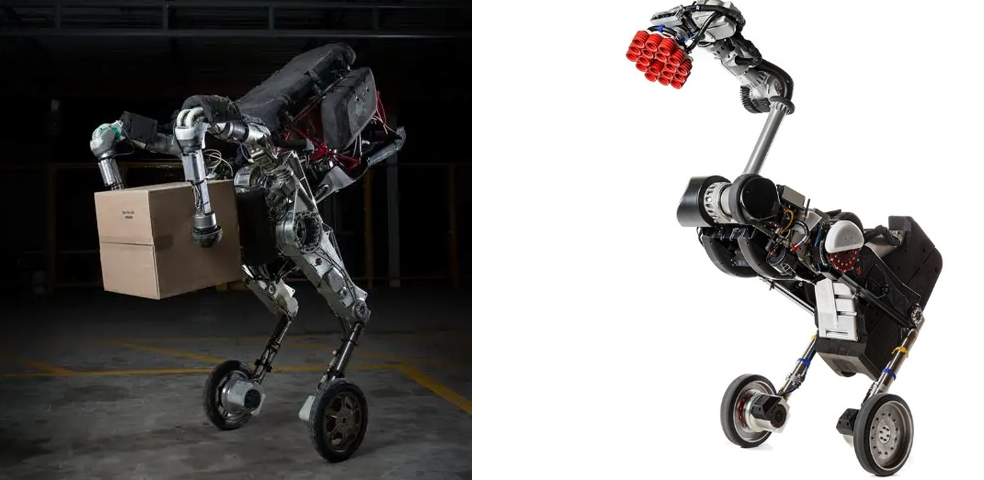
\includegraphics[width=0.7\textwidth]{figures/ch01/image3.png}
  \caption{一代 Handle 机器人（左），二代 Handle 机器人（右）\cite{boston2023handle,boston2023stretch}}
  \label{fig:handle}
\end{figure}

\begin{figure}[H]
  \centering
  \begin{minipage}[b]{0.4\textwidth}
    \centering
    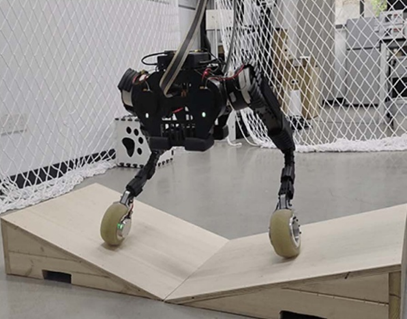
\includegraphics[width=\textwidth]{figures/ch01/image4.png}
  \end{minipage}
  \begin{minipage}[b]{0.4\textwidth}
    \centering
    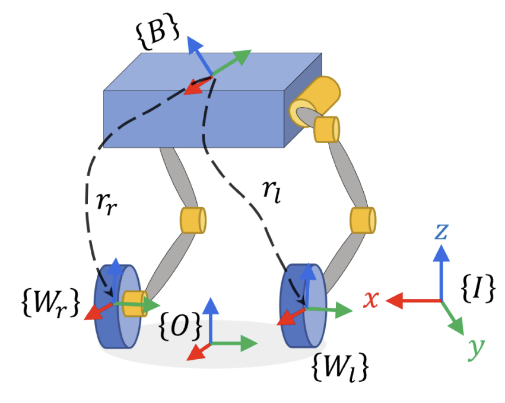
\includegraphics[width=\textwidth]{figures/ch01/image5.png}
  \end{minipage}
  \caption{HotWheel 机器人\cite{yu2023hotwheel}}
  \label{fig:hotwheel-serial}
\end{figure}

\begin{figure}[H]
  \centering
  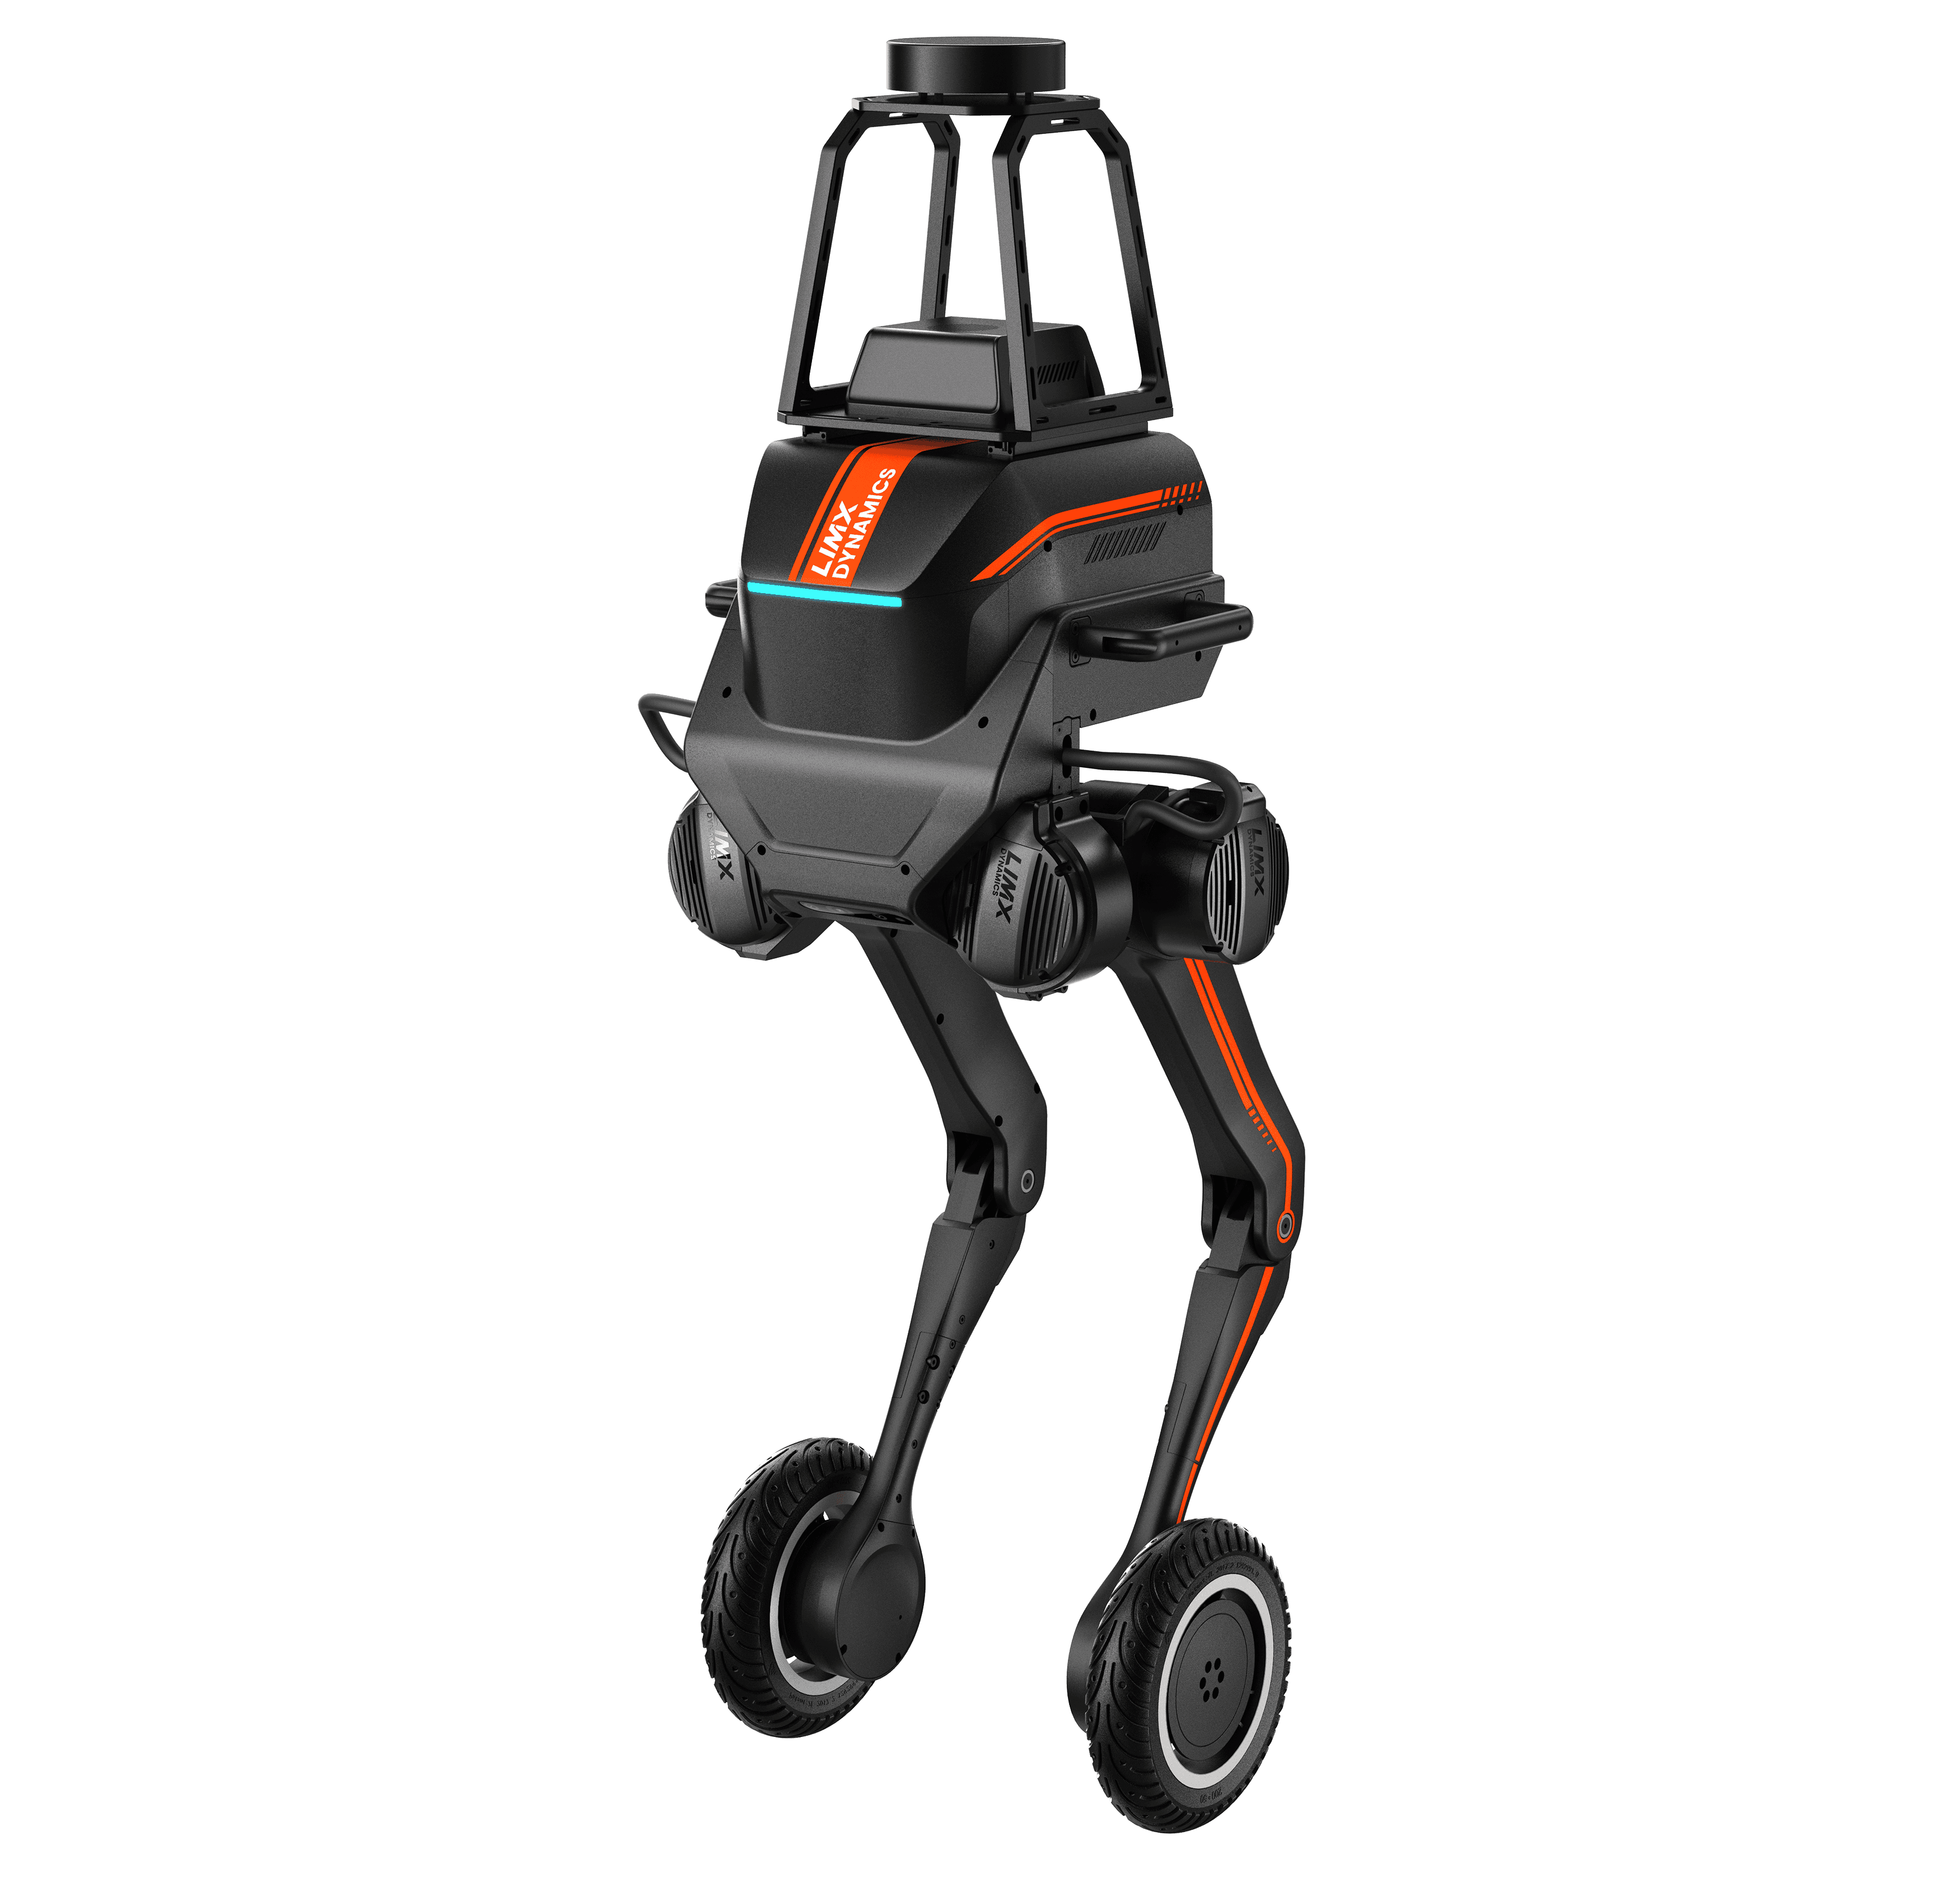
\includegraphics[width=0.5\textwidth]{figures/ch01/image6.png}
  \caption{TRON 1 机器人\cite{limx2025tron1}}
  \label{fig:tron1}
\end{figure}

上述平台的共性问题在于：开链结构导致腿部转动惯量偏高，串联关节逐级累积误差降低了整机刚度与末端定位精度。本文在机械设计中同样采用了串联主链以保留工作空间优势，但通过引入局部闭环支链来分担关节负载和提升侧向刚度，正是针对上述不足的改进尝试。

\subsubsection{并联结构}

并联构型以闭链机构提供高刚度和强承载能力，但工作空间受限。Sugahara 与 Hashimoto 团队在 2004--2005 年开发的 WL-16 与 WS-2 组合系统\cite{sugahara2004,hashimoto2005}（\figref{fig:ws2-wl16}）采用 6 自由度并联腿，通过切换足底橡胶垫的收放实现步态与轮式移动的切换，是早期轮足复合的代表。ETH Zurich 2019 年推出的 Ascento\cite{klemm2019ascento}（\figref{fig:ascento}）采用闭式四连杆机构，轮心近似直线运动，有效解耦了跳跃与平衡控制，并通过拓扑优化实现轻量化。腾讯 2021 年发布的 Ollie\cite{wang2021ollie}（\figref{fig:ollie}）采用对称五连杆设计，单腿集成一个轮毂电机与两个关节电机，腹部飞轮用于补偿空中姿态，能以 0.35\,m 最低身高完成空翻和跳跃。

\begin{figure}[H]
  \centering
  \begin{minipage}[b]{0.22\textwidth}
    \centering
    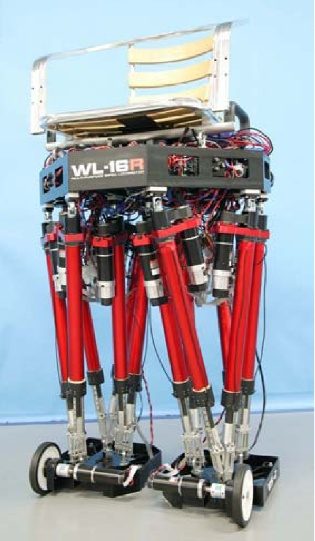
\includegraphics[width=\textwidth]{figures/ch01/image7.jpeg}
  \end{minipage}
  \begin{minipage}[b]{0.45\textwidth}
    \centering
    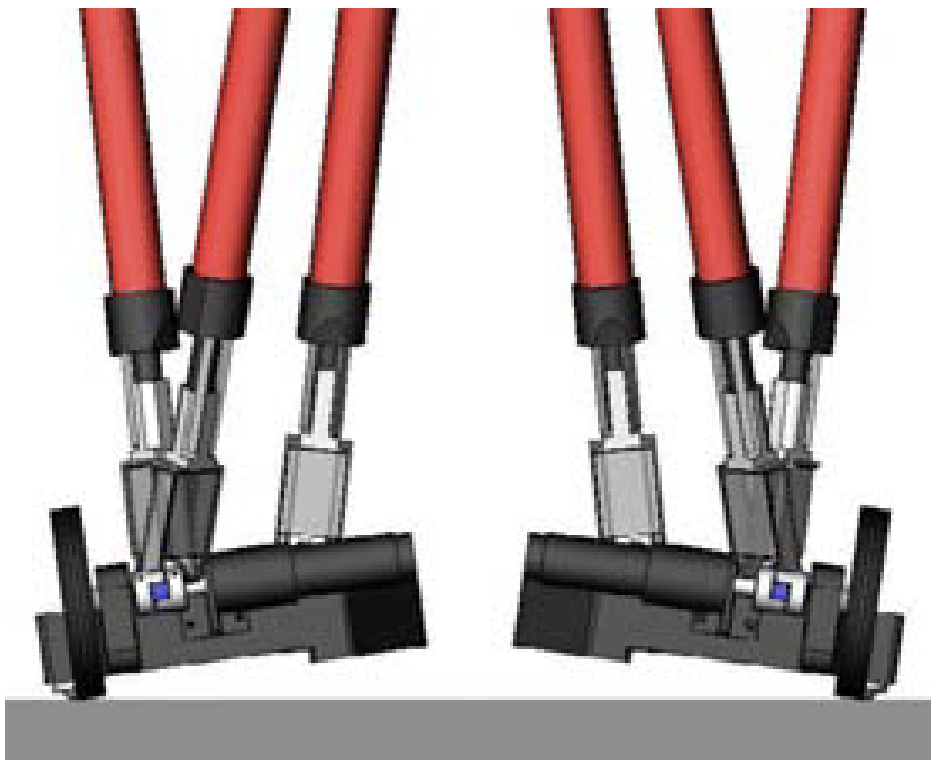
\includegraphics[width=\textwidth]{figures/ch01/image8.png}
  \end{minipage}
  \caption{WS-2 / WL-16\cite{sugahara2004,hashimoto2005}}
  \label{fig:ws2-wl16}
\end{figure}

\begin{figure}[H]
  \centering
  \begin{minipage}[b]{0.35\textwidth}
    \centering
    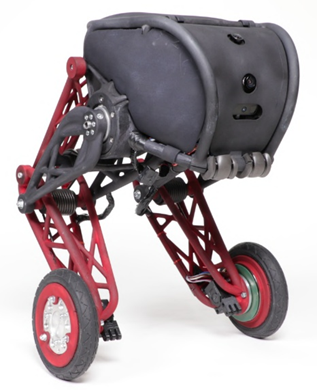
\includegraphics[width=\textwidth]{figures/ch01/image9.png}
  \end{minipage}
  \begin{minipage}[b]{0.5\textwidth}
    \centering
    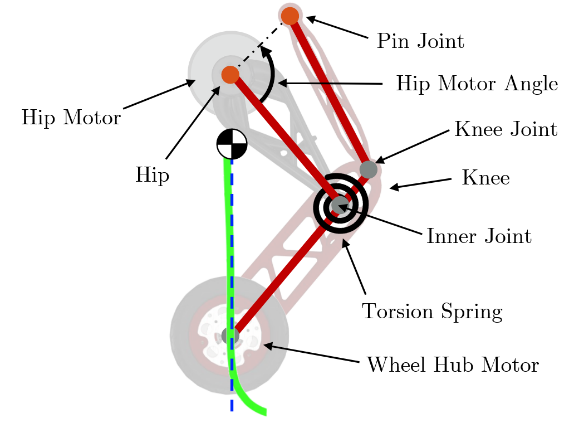
\includegraphics[width=\textwidth]{figures/ch01/image10.png}
  \end{minipage}
  \caption{Ascento 机器人\cite{klemm2019ascento}}
  \label{fig:ascento}
\end{figure}

\begin{figure}[H]
  \centering
  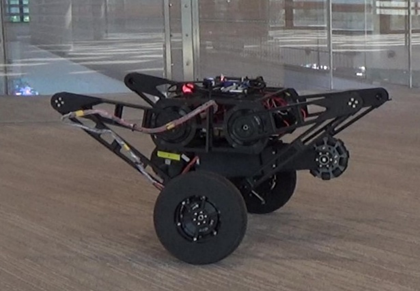
\includegraphics[width=0.52\textwidth]{figures/ch01/image11.png}
  \caption{Ollie 机器人\cite{wang2021ollie}}
  \label{fig:ollie}
\end{figure}

并联构型的共性局限在于：闭链结构天然限制了腿长变化范围和越障高度，且对加工精度与装配误差敏感。Ascento 的有效腿长变化有限，不适合大幅度高度调节；Ollie 依赖额外飞轮补偿空中姿态，增加了控制维度。本文在腿部设计中保留并联支链以获取结构刚度，同时通过将其等效为可伸缩虚拟腿，在任务空间中回避了闭链运动学的复杂性——这在建模思路上与 Ascento 的虚拟腿抽象类似，但在机构形式上以五连杆替代了四连杆。

\subsubsection{混合式结构}

2021 年开源项目 Stanley\cite{stanley2025}（\figref{fig:stanley}）的腿部在运动学上为三自由度串联链，但髋、膝关节的驱动电机并联布置于机身内部，通过绞盘和线缆远程传动，降低了腿部惯量。上海交通大学交龙战队 2025 年开源的双轮足机器人\cite{sjtu2025rm}（\figref{fig:sjtu-hybrid-leg}）同样采用”宏观串联、驱动并联”的混合构型，通过相似连杆机构实现并联传动，并利用导电滑环实现 360° 全向旋转和倒地自起。

\begin{figure}[H]
  \centering
  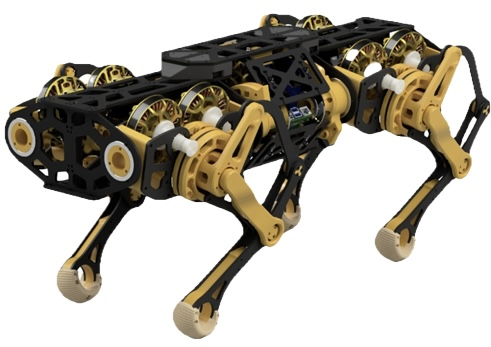
\includegraphics[width=0.38\textwidth]{figures/ch01/image12.jpg}
  \caption{Stanley 机器人\cite{stanley2025}}
  \label{fig:stanley}
\end{figure}

\begin{figure}[H]
  \centering
  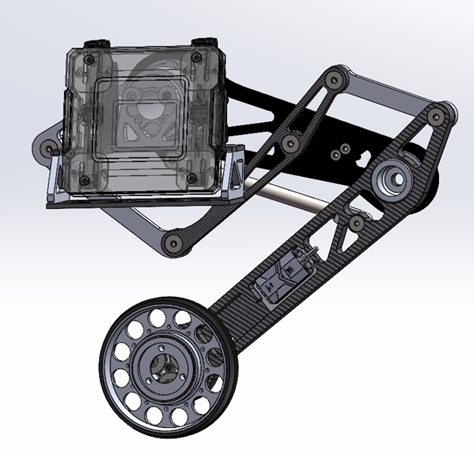
\includegraphics[width=0.4\textwidth]{figures/ch01/image13.png}
  \caption{混合式构型腿部\cite{sjtu2025rm}}
  \label{fig:sjtu-hybrid-leg}
\end{figure}

从上述平台来看，现有混合式方案侧重于将驱动并联化以降低腿部惯量，其闭环支链主要在传动端发挥作用，尚未将并联结构的承载能力直接转化为对轮地接触力和侧向刚度的增强。此外，目前多数平台面向高性能验证或开源竞赛场景，尺寸偏大，缺少面向小型化原型验证的紧凑设计。本文的混合式腿部机构同样遵循”串联主链 + 并联闭环支链”的思路，但将闭环支链直接作用于负载分担和结构刚度提升，而非仅用于传动解耦，这在机构功能定位上与 Stanley 和交龙方案有所区别。

\subsection{运动控制}

双轮足机器人的控制策略融合了轮式平衡与腿式运动两类方法，LQR、VMC、MPC、WBC 和强化学习等均有应用。

Pratt 等人于 2001 年提出虚拟模型控制（VMC）\cite{pratt2001}（\figref{fig:spring-turkey-vmc}），通过模拟虚拟弹簧-阻尼等力学元件直接生成关节力矩，将高层任务描述转化为底层力控指令，显著降低了计算需求。本文的腿长支撑控制直接沿用了这一思想。Sentis 于 2005 年提出全身控制（WBC）框架\cite{sentis2005}，以零空间投影实现多任务的优先级分层，将关节限位、接触约束等硬约束嵌入优化问题，为轮腿系统的多任务协调提供了理论框架。

\begin{figure}[H]
  \centering
  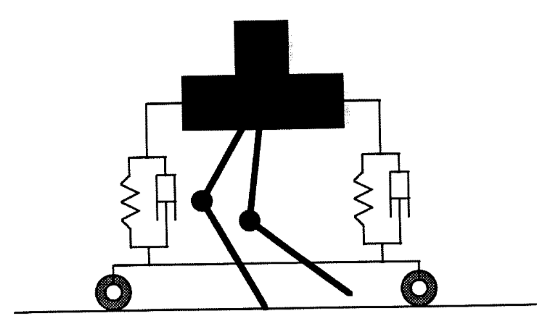
\includegraphics[width=0.6\textwidth]{figures/ch01/image14.png}
  \caption{搭载虚拟助行架的 Spring Turkey 机器人\cite{pratt2001}}
  \label{fig:spring-turkey-vmc}
\end{figure}

在轮式双足机器人的具体应用中，控制方法呈现两条主线。一是以 WBC/MPC 为代表的优化型方法：Klemm 2020 将 LQR 反馈律嵌入 WBC 层级应用于 Ascento\cite{klemm2020lqr}（\figref{fig:lqr-wbc-ascento}），通过闭环力解析解处理腿部运动学闭环，以 ZMP 调节侧倾角抑制侧翻；Wang 2022 提出 MFT-WBC\cite{wang2022mft}（\figref{fig:mft-wbc}），将机构可传递性指标离线建模为多面体约束集成到在线 QP 中，实现了 1\,kHz 伺服速率；Zhang 2022 将自适应动态规划（ADP）与 WBC 结合应用于 Ollie\cite{zhang2022ollie}（\figref{fig:ollie-control-framework}），在线更新控制策略以适应参数变化；Yu 2023 提出轮式刚体动力学（WRBD）模型并结合 MPC 实现 HotWheel 的 6 自由度位姿跟踪\cite{yu2023hotwheel}（\figref{fig:hotwheel-control-framework}）。上述方法的共性是依赖在线优化求解，计算复杂度较高。二是面向特定任务的专项控制：Xia 2025 为双轮足机器人建立了空中动力学模型并设计了跳跃姿态控制器\cite{xia2025jump}（\figref{fig:jump-planning}），验证了基于模型的专项控制在特定动作中的有效性。

\begin{figure}[H]
  \centering
  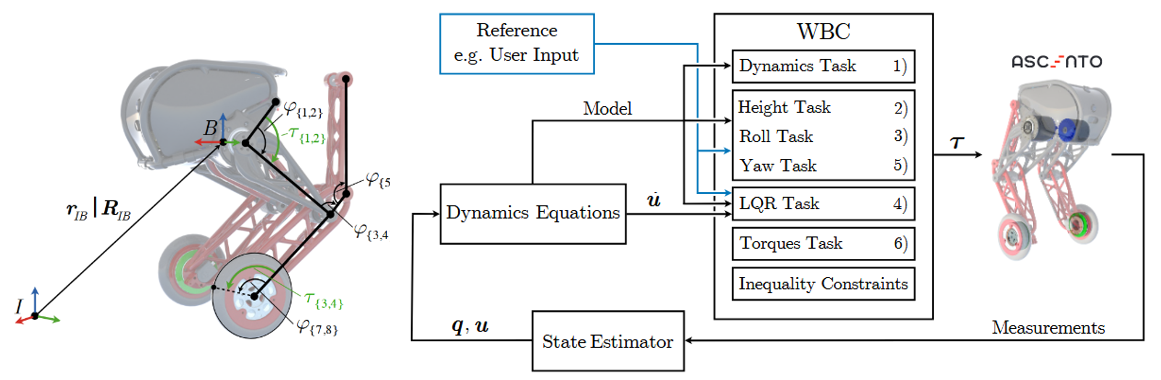
\includegraphics[width=1.0\textwidth]{figures/ch01/image15.png}
  \caption{腿部连杆运动闭环（左），LQR-WBC 控制框架（右）\cite{klemm2020lqr}}
  \label{fig:lqr-wbc-ascento}
\end{figure}

\begin{figure}[H]
  \centering
  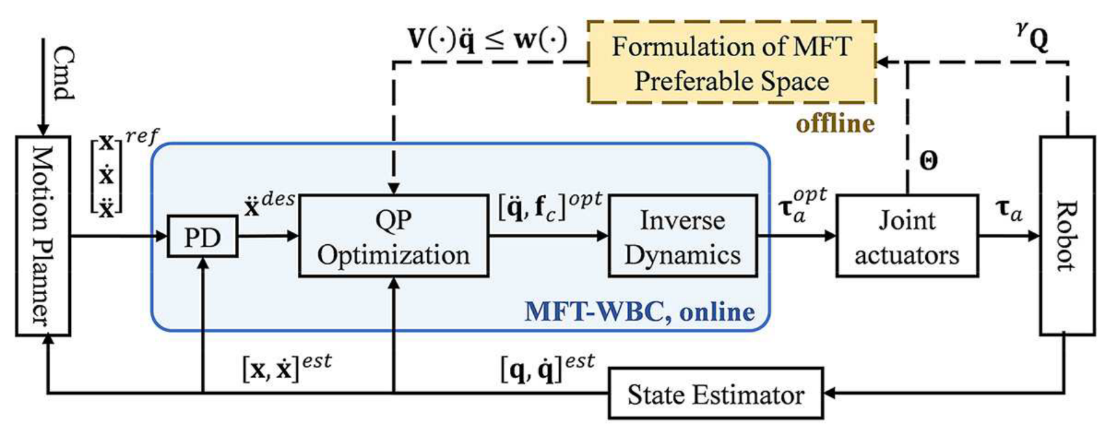
\includegraphics[width=0.72\textwidth]{figures/ch01/image16.png}
  \caption{MFT-WBC 控制框架\cite{wang2022mft}}
  \label{fig:mft-wbc}
\end{figure}

\begin{figure}[H]
  \centering
  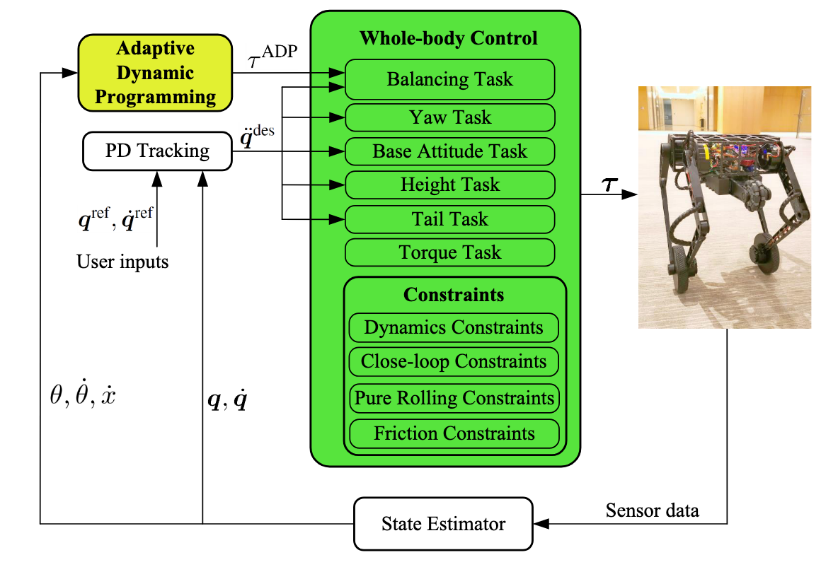
\includegraphics[width=0.65\textwidth]{figures/ch01/image17.png}
  \caption{Ollie 的控制框架\cite{zhang2022ollie}}
  \label{fig:ollie-control-framework}
\end{figure}

\begin{figure}[H]
  \centering
  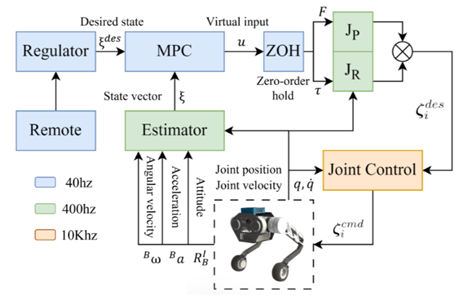
\includegraphics[width=0.7\textwidth]{figures/ch01/image18.png}
  \caption{HotWheel 控制框架\cite{yu2023hotwheel}}
  \label{fig:hotwheel-control-framework}
\end{figure}

\begin{figure}[H]
  \centering
  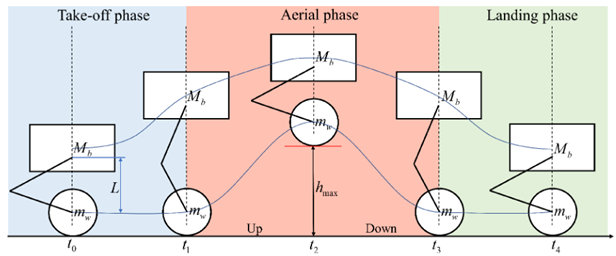
\includegraphics[width=0.8\textwidth]{figures/ch01/image19.png}
  \caption{跳跃过程及轨迹规划示意图\cite{xia2025jump}}
  \label{fig:jump-planning}
\end{figure}

综合来看，优化型方法性能优异但计算成本高，专项控制轻量但覆盖范围有限。本文的分层 LQR-VMC 方案试图在两者之间取折中——以非优化途径实现平衡、腿长支撑和侧向稳定三项核心功能，在不引入在线优化的前提下获得可接受的综合性能。

\begin{table}[H]
  \centering
  \caption{双轮足机器人主流控制方法对比}
  \label{tab:control-method-overview}
  \small
  \begin{tabular}{p{0.9cm}p{2.5cm}p{2.3cm}p{2.5cm}p{3.2cm}}
    \toprule
    方法 & 核心思想 & 优势 & 局限 & 嵌入式实时适用性 \\
    \midrule
    LQR & 平衡点附近线性二次型最优 & 离线求解、在线计算量低 & 需线性化假设，对强非线性适应性有限 & 良好——仅需矩阵乘法 \\
    \hline
    VMC & 虚拟弹簧-阻尼等力学元件直接构造控制量 & 物理直觉强、无需精确模型 & 缺乏多任务协调机制 & 良好——闭式代数运算 \\
    \hline
    WBC & 多任务分层优化，约束优先级处理 & 约束处理完善、多任务协调 & 依赖精确模型 + QP 在线求解 & 较差——每步需解 QP \\
    \hline
    MPC & 滚动时域优化，显式处理约束与预测 & 预测能力强、可处理约束 & 计算量大，对模型精度要求高 & 待提升——TinyMPC 等轻量求解器尚未在轮腿系统验证 \\
    \hline
    RL & 数据驱动、端到端学习控制策略 & 无需显式建模 & 训练数据量大、sim-to-real 差距、可解释性弱 & 部署后可实时推理，但训练阶段成本极高 \\
    \bottomrule
  \end{tabular}
\end{table}

从表\ref{tab:control-method-overview} 可见，WBC 和 MPC 的优越性能以高昂的在线计算为代价，RL 则将复杂性转移到训练阶段。面向嵌入式实时控制的工程需求，LQR 和 VMC 的低计算成本优势突出——前者离线求解 Riccati 方程，在线仅需计算恒定增益矩阵的乘法；后者为闭式代数运算，无需迭代。LQR 和 VMC 的结合能够在保持平衡和腿长支撑两个方向上分别发挥各自优势，且不引入在线优化环节，这正是本文选择 LQR-VMC 分层架构作为控制方案的核心考量。

\subsection{现有研究存在的问题}

现有研究在双轮足机器人的机构设计与控制方法上已取得显著进展，但以下问题仍有待进一步解决。

机械结构方面：串联构型工作空间大，但腿部转动惯量高、刚度不足；并联构型承载能力强、结构紧凑，但运动范围受限、机构复杂。近年来，简化腿部机构以降低驱动与建模复杂度成为一种趋势。Liu 等人在 IROS 2024 提出的 DIABLO 机器人\cite{liu2024diablo} 采用全直驱关节设计，将串联腿部简化为 6 个无减速器电机，并以二阶倒立摆近似其动力学，实现了基于 LQR 的平衡控制。该设计在降低结构复杂度上迈出了重要一步，但其腿部本质上仍为串联构型，未引入并联支链分担关节负载或提升侧向刚度。混合式构型虽试图兼顾两者优势，但现有平台多面向高性能样机验证，在紧凑化、低成本实现方向上的探索尚不充分。

控制方法方面：WBC、MPC 和强化学习等主流策略在复杂任务中控制效果突出，但对高精度模型、在线优化计算或大量训练数据的依赖，使它们在嵌入式平台上面临部署困难、实时性不足等问题。Yu 等人提出的分层 MPC 框架\cite{yu2023mpc} 借助虚拟模型控制思想忽略腿部动力学以降低模型阶数，但 MPC 滚动优化所需的在线求解仍对算力构成较大负担。Nguyen 等人提出的 TinyMPC\cite{nguyen2024tinympc} 获 ICRA 2024 最佳论文奖，通过 ADMM 算法将 MPC 求解压缩至微控制器级别，验证了轻量化优化的可行性，但该方法目前仅在四旋翼上完成验证，尚未拓展至轮腿系统。在 LQR-VMC 混合架构方向上，Yang 等人提出的集成建模与控制优化方案\cite{yang2024integrated} 采用了自适应 LQR 与轨迹方程加速 VMC 相结合的框架，在思路上与本文相近，但其工作以仿真为主，物理实验部分较为初步，缺少完整的闭环验证。对于以工程实现为目标的双轮足机器人，能否在保持平衡、越障和侧向稳定性的同时，降低控制算法的复杂度与实现门槛，仍是一个尚未充分解决的问题。

\section{本文主要研究内容及章节安排}

本文围绕小型混合式双轮足机器人，从机械结构设计、运动学与动力学建模、分层控制方法和实验验证四个方面开展工作。

机械结构方面，完成了整机总体方案与混合式闭环腿部机构设计，以及传动系统、驱动系统的选型与校核，确定了关键结构参数与执行器型号。建模分析方面，建立了机器人的平面等效运动学与动力学模型，推导了面向 LQR 的线性化状态空间表达式，并给出了五连杆机构从任务空间到关节空间的力矩映射关系。控制方法方面，提出了 LQR-VMC 分层控制方案：LQR 负责平衡控制、速度跟踪和腿摆力矩分配，VMC 负责腿长方向的虚拟弹簧-阻尼支撑，同时引入基于滚转角的腿长差修正项以增强侧向姿态的稳定性。在上述工作的基础上，通过仿真和物理样机实验，对原地平衡、速度跟踪、扰动恢复、腿长调节和滚转稳定等典型工况进行了验证。

全文共分为六章，各章节内容安排如下：

第1章为绪论，介绍研究背景与意义，综述双轮足机器人在机械结构与运动控制方面的研究进展，分析现有不足，明确本文的研究内容、技术路线与创新点。

第2章阐述整机总体方案与混合式腿部机构设计，涵盖躯干结构、传动系统、驱动系统及控制硬件的选型与设计，给出关键参数。

第3章建立机器人的平面等效运动学与动力学模型，推导线性化状态空间方程与任务空间到关节空间的力矩映射，为控制器设计提供模型基础。

第4章设计 LQR-VMC 分层控制器，给出状态估计与控制流程，并通过 MuJoCo 仿真验证闭环性能。

第5章在物理样机上开展实验，覆盖原地平衡、速度跟踪、腿长控制和滚转稳定等工况，评估控制器在实际硬件上的性能与稳定性。

第6章总结全文工作与结论，指出当前方法的局限性，展望后续改进方向。

\begin{figure}[H]
  \centering
  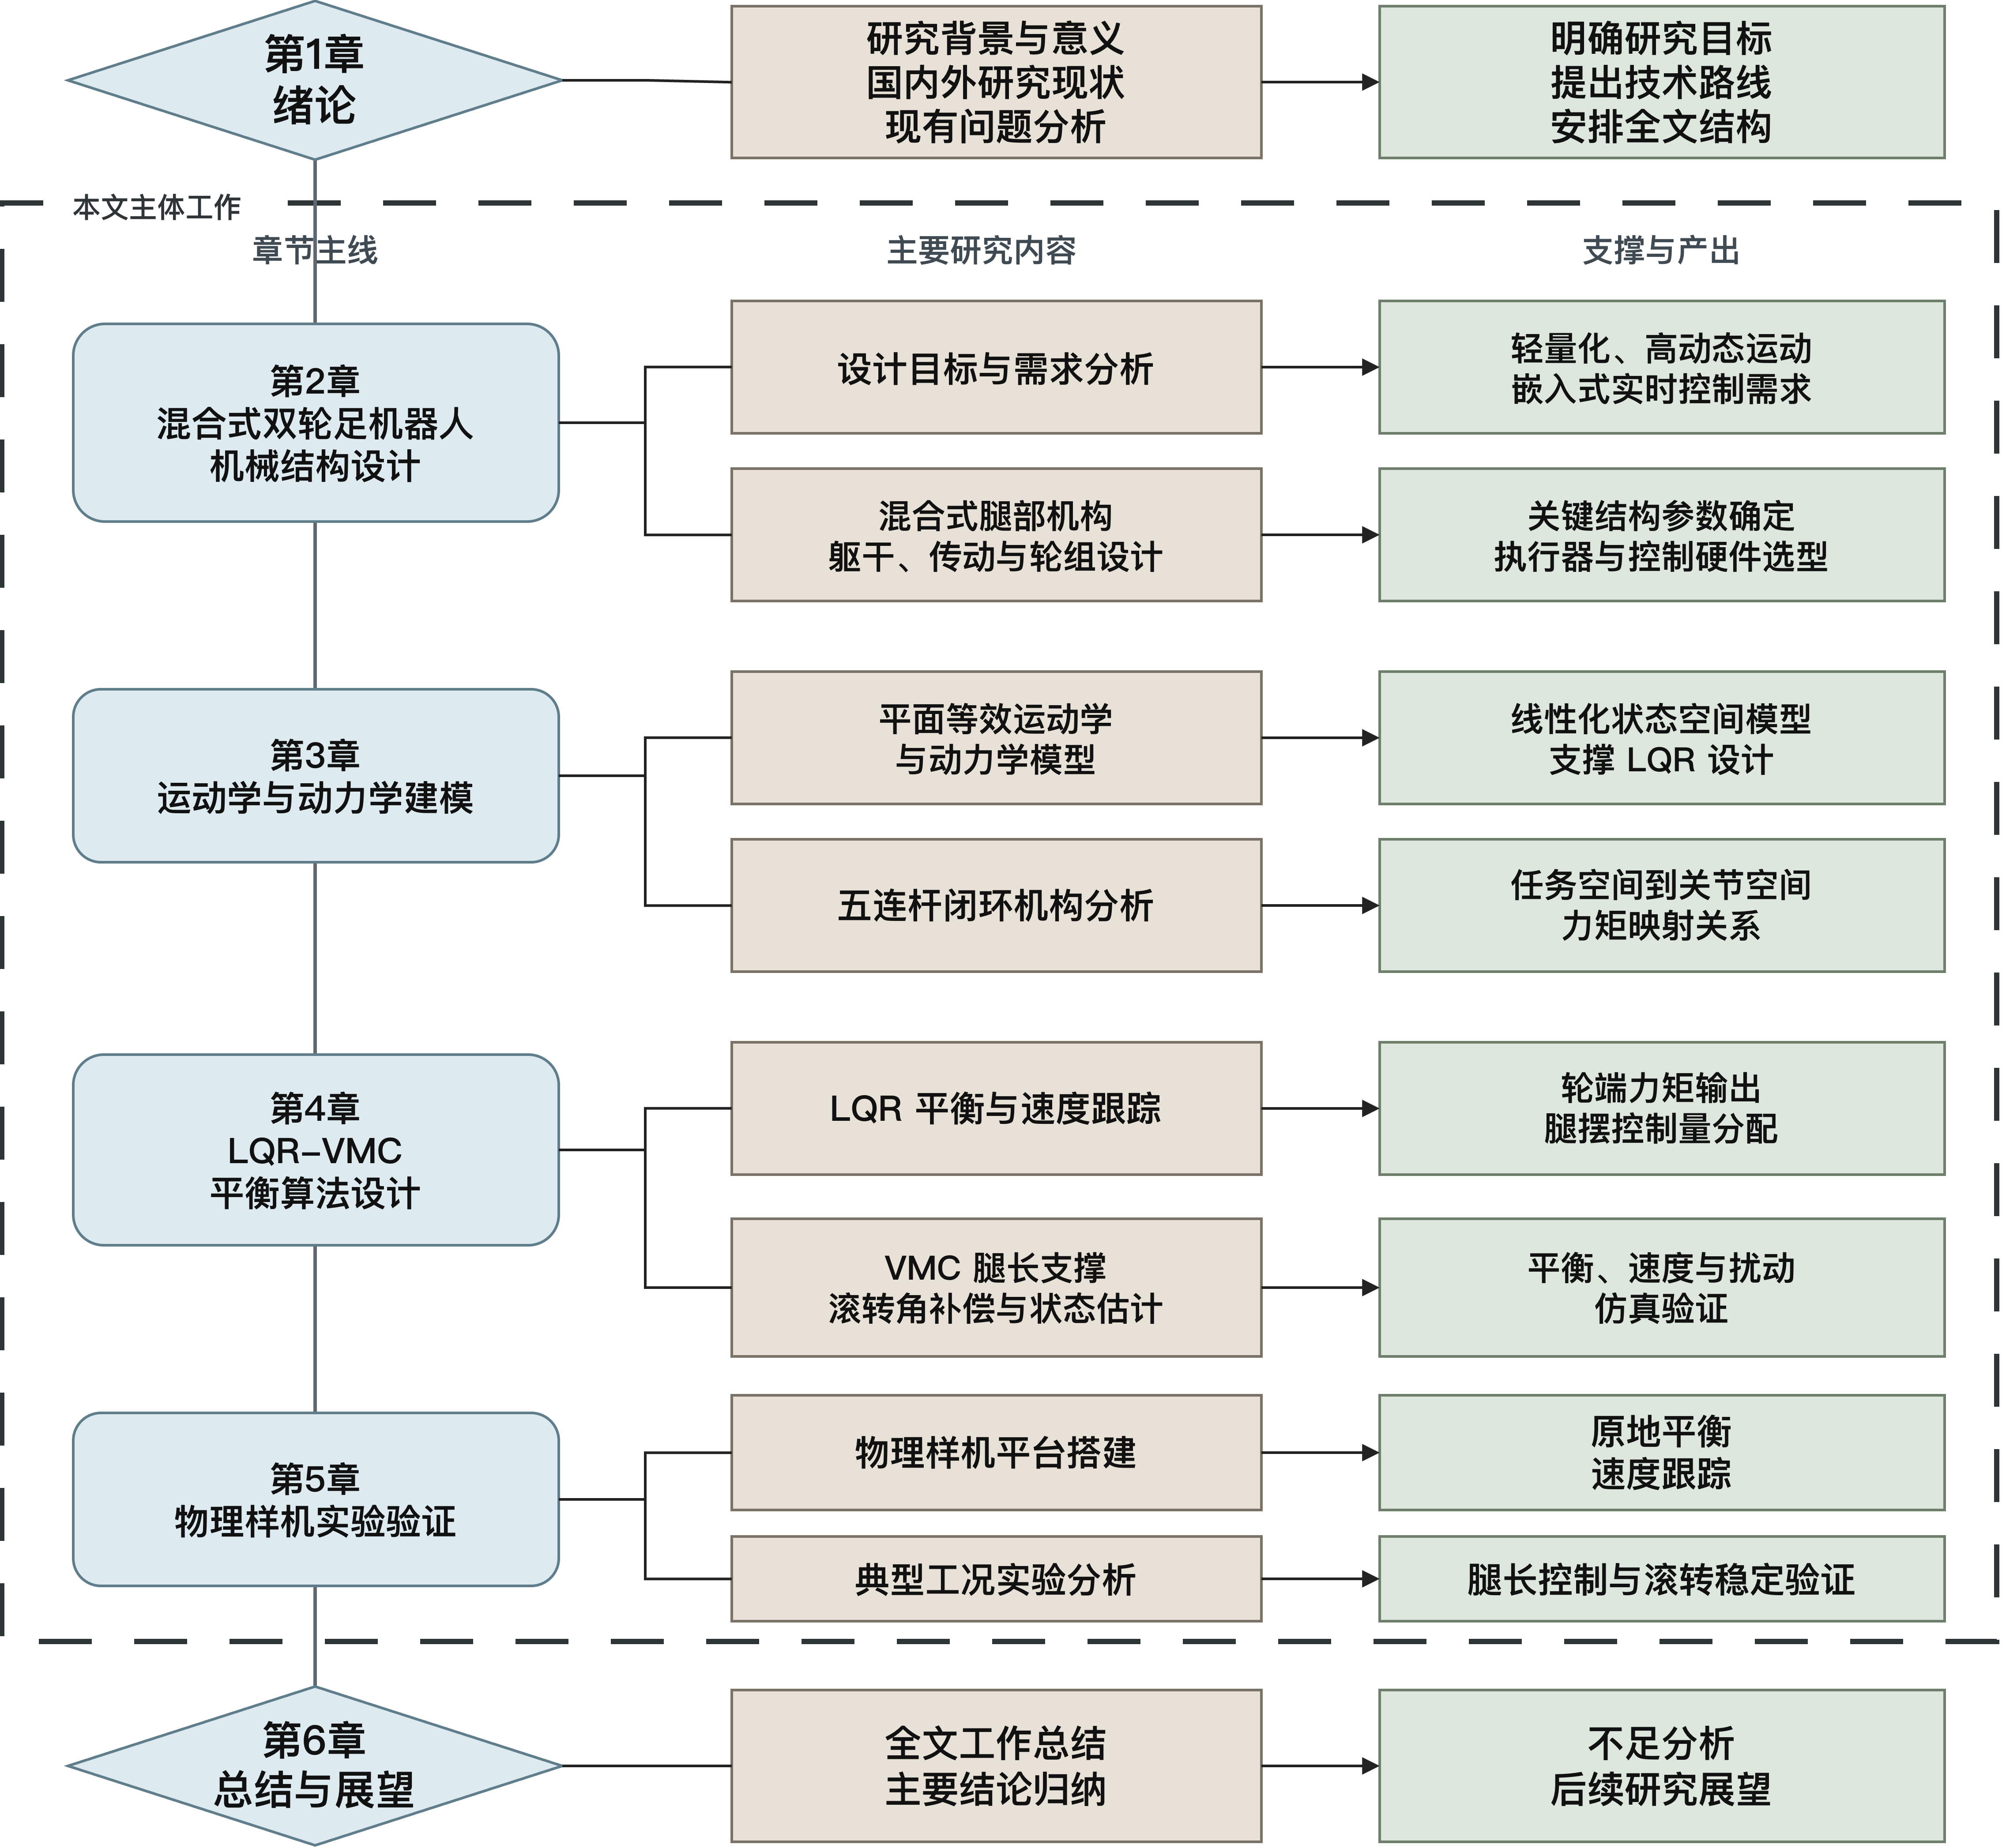
\includegraphics[width=0.9\textwidth]{figures/ch01/research_architecture.png}
  \caption{论文研究内容与技术路线}
  \label{fig:research-architecture}
\end{figure}

\chapter{混合式双轮足机器人机械结构设计}\label{chap:mechanism}

双轮足机器人的控制效果很大程度上取决于机械本体。若腿部惯量过大、传动回差明显，后续的平衡控制和腿长调节都会变得困难。因此，本章先给出样机的设计指标，再说明腿部、躯干、传动、轮组、电机和传感器的具体选型，为第三章建模提供必要的结构参数。

\section{设计目标与需求分析}

样机主要面向平地移动、低台阶越障和原地平衡等场景。与四足轮腿平台相比，双轮足结构的执行器数量较少，整机也更紧凑；相应地，它对重心位置、腿部刚度和姿态反馈更敏感。结合后续控制实验的需要，机械设计需满足以下要求：

\begin{enumerate}
  \item 移动与越障能力：机器人在轮式支撑状态下应能达到目标速度，并通过腿部伸缩完成低台阶越障和落地缓冲。
  \item 轻量化：整机质量控制在较低水平，尤其要减小腿部运动件的转动惯量，避免电机长期工作在高负载区间。
  \item 刚度与装配精度：腿部机构、髋部轴系和传动系统需有足够刚度，传动间隙也应控制在可接受范围内。
  \item 集成与维护：躯干需要容纳电池、主控板、驱动器和传感器，并留出装配、走线和后续调试空间。
  \item 便于建模：机械构型应能用虚拟腿长和虚拟腿摆角描述，以便第三章建立任务空间模型。
\end{enumerate}

样机预期性能指标见\tabref{tab:design-targets}。其中，整机质量和自由度用于限制平台复杂度，移动速度和越障高度对应主要运动能力，连续工作时间用于约束电池和整机效率。

\begin{table}[H]
  \centering
  \caption{样机预期性能指标}\label{tab:design-targets}
  \renewcommand{\arraystretch}{1.3}
  \begin{tabular}{p{3cm}p{3cm}p{7cm}}
    \toprule
    指标名称 & 期望目标值 & 说明 \\
    \midrule
    整机质量 & $\leq 5\,\mathrm{kg}$ & 降低惯性和能耗，提高平衡控制响应速度 \\
    移动速度 & $\geq 2\,\mathrm{m/s}$ & 轮式移动能力要求 \\
    可跨越台阶高度 & $\geq 10\,\mathrm{cm}$ & 腿部伸缩能力要求 \\
    自由度 & $6\,\mathrm{DOF}$ & 左右腿部驱动与双轮驱动的基本配置 \\
    连续工作时间 & $\geq 30\,\mathrm{min}$ & 电池容量和整机效率约束 \\
    \bottomrule
  \end{tabular}
\end{table}

总体结构由躯干、左右对称腿部模块和两个驱动轮组成。腿部采用混合式闭环连杆机构，在串联主链中加入局部并联支链，以兼顾运动范围和支撑刚度。腿部驱动电机布置在靠近躯干的位置，通过链传动带动连杆运动；轮毂电机布置在足端，用于平地移动和差速转向。

\section{腿部结构设计}

腿部结构决定了越障高度、支撑刚度以及后续任务空间变量的定义。每条腿由髋部基座、主动曲柄、从动连杆、闭环支链和足端轮组构成。该结构保留了串联腿的运动范围，同时通过闭环支链提高局部刚度，适合小型双轮足样机。

\begin{figure}[H]
  \centering
  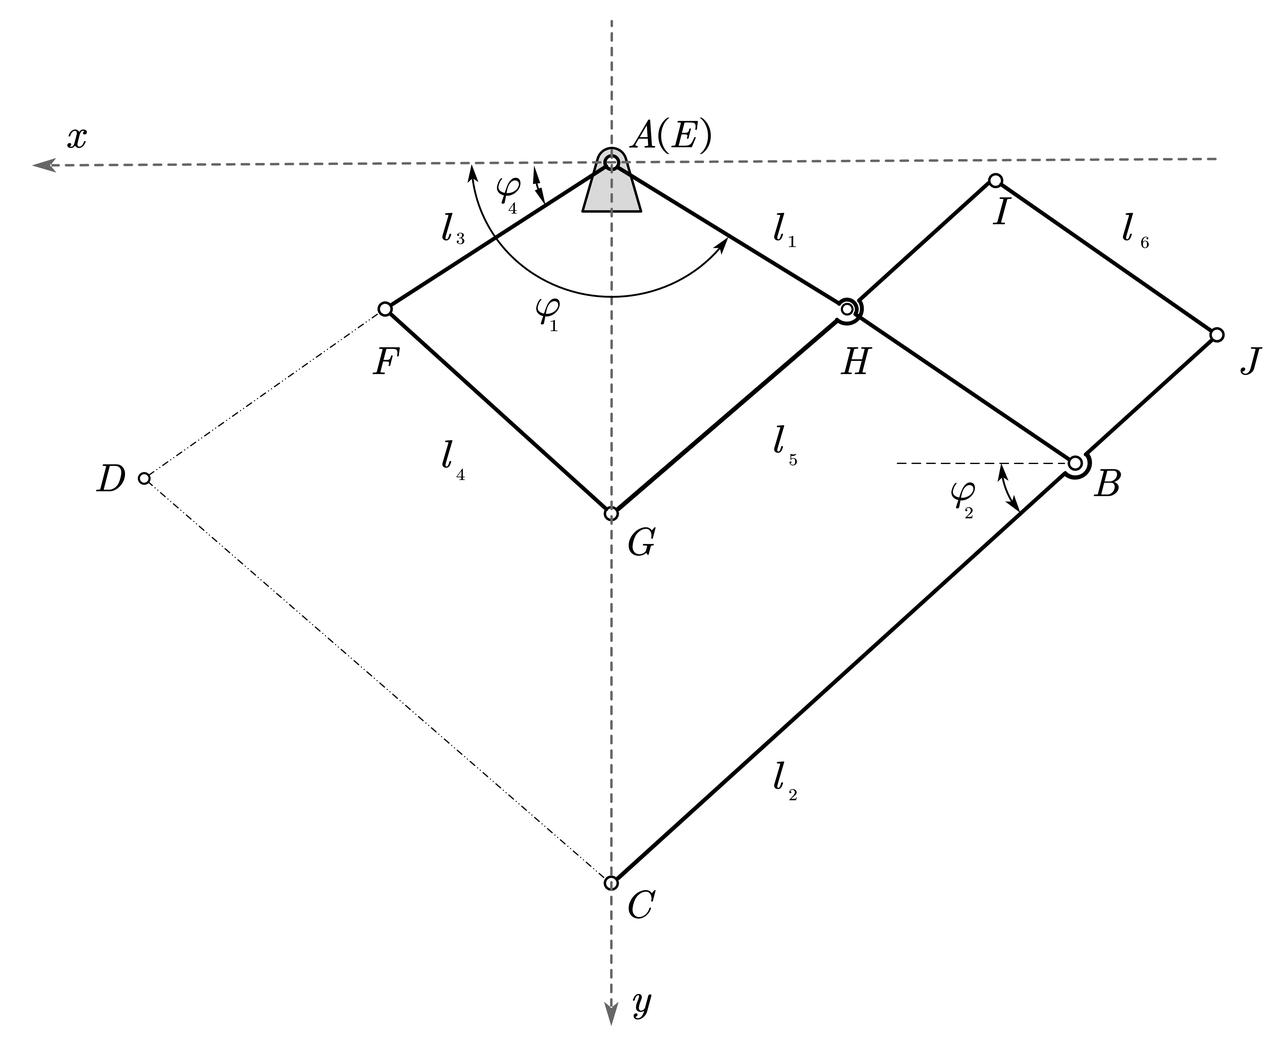
\includegraphics[width=0.52\textwidth]{figures/ch02/image1.png}
  \caption{腿部连杆机构简图}
  \label{fig:leg-linkage}
\end{figure}

为减小腿部转动惯量，腿部主要驱动电机布置在髋关节附近，并尽量靠近躯干。这样在摆腿、落地缓冲和越障时，质量较大的电机本体不随足端大幅运动，可降低惯性力矩和冲击载荷。足端轮组同时承担支撑和驱动作用，与连杆机构一起构成轮足复合运动单元。

根据整机尺寸和越障指标，腿部连杆尺寸需要同时满足伸展高度、收缩高度和传动角约束。选取的关键尺寸如下：

\begin{itemize}
  \item 驱动曲柄长度：$AF = AH = 86.4\,\mathrm{mm}$，该尺寸影响腿部摆动幅度和电机输出端力臂。
  \item 从动连杆长度：$CJ = 250.16\,\mathrm{mm}$，该尺寸用于保证足端伸展范围。
  \item 主支撑杆长度：$GI = 160\,\mathrm{mm}$，该尺寸用于形成主要承载支链。
\end{itemize}

当腿部机构接近最大伸展姿态时，可估算足端最大高度为

\begin{equation}
  H_{\max} = AB + BC = 160 + 196 = 356\,\mathrm{mm}.
\end{equation}

受机械限位和传动角限制，设定曲柄向上旋转的极限夹角约为水平以上 $30^\circ$，此时腿部最小收缩高度约为

\begin{equation}
  H_{\min} \approx 100\,\mathrm{mm}.
\end{equation}

由此得到腿部有效伸缩行程为

\begin{equation}
  S_{\mathrm{eff}} = H_{\max} - H_{\min} \approx 256\,\mathrm{mm}.
\end{equation}

该行程大于\tabref{tab:design-targets}中的越障高度指标，也为落地缓冲和高度调节留出余量。由上述参数得到的腿部工作空间如\figref{fig:leg-workspace}所示，足端在竖直方向上的可达范围满足后续虚拟腿建模需要。

\begin{figure}[H]
  \centering
  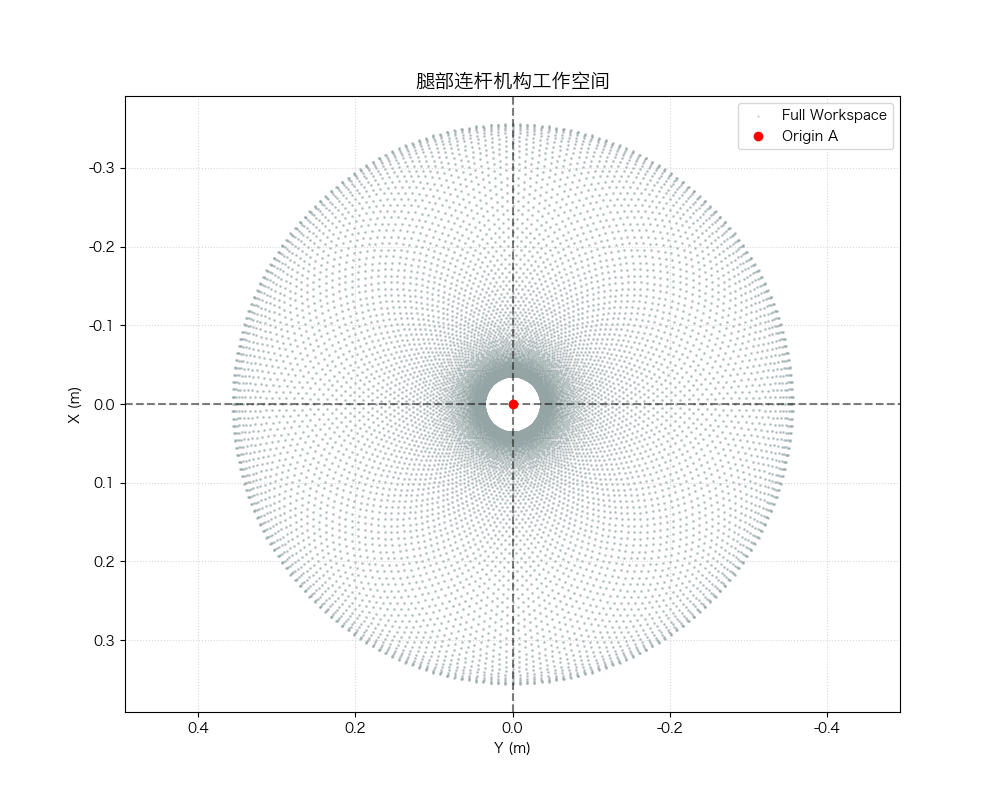
\includegraphics[width=0.72\textwidth]{figures/ch02/image2.png}
  \caption{腿部连杆工作空间示意图}
  \label{fig:leg-workspace}
\end{figure}

腿部连杆参数汇总如\tabref{tab:link-lengths}所示。第三章将根据这些几何参数建立闭环运动学模型。

\begin{table}[H]
  \centering
  \caption{腿部连杆参数汇总}\label{tab:link-lengths}
  \renewcommand{\arraystretch}{1.2}
  \begin{tabular}{cc}
    \toprule
    连杆代号 & 长度/m \\
    \midrule
    AF & 0.08640 \\
    FG & 0.10584 \\
    GI & 0.16000 \\
    IJ & 0.07360 \\
    JC & 0.25016 \\
    AB & 0.16000 \\
    \bottomrule
  \end{tabular}
\end{table}

\begin{figure}[H]
  \centering
  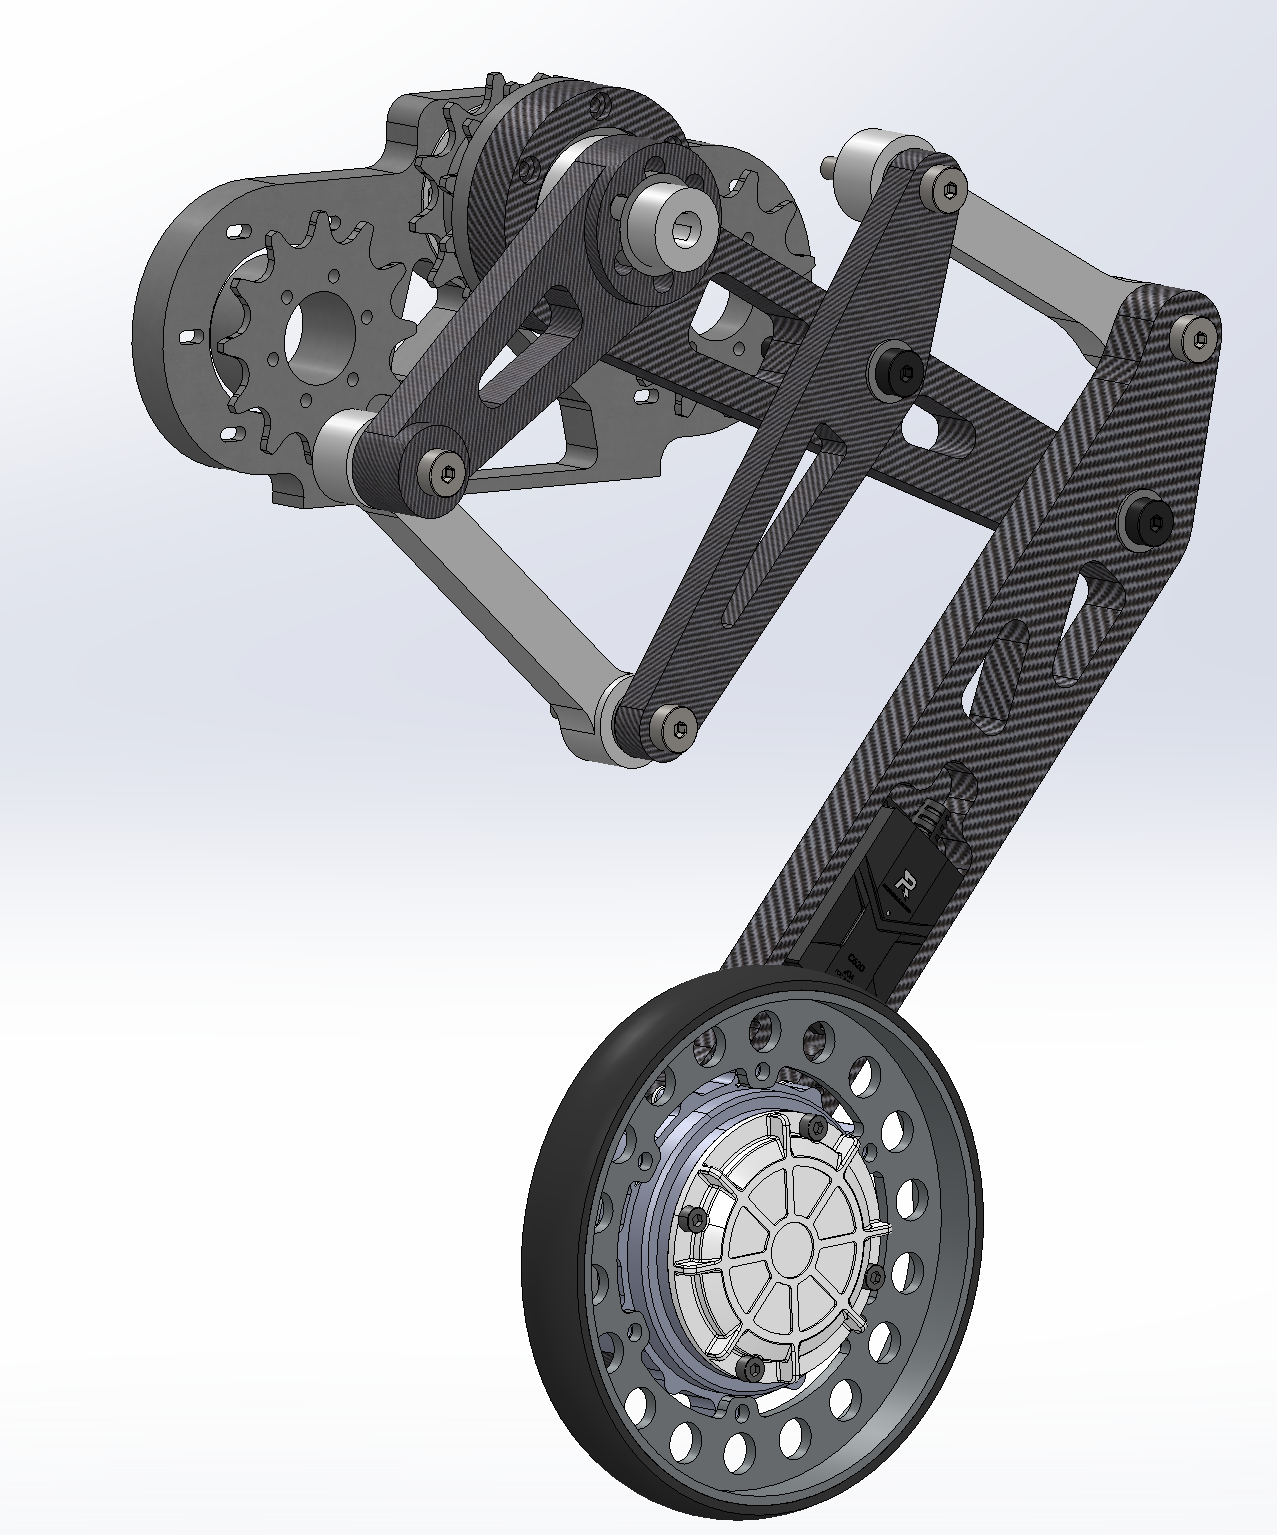
\includegraphics[width=0.6\textwidth]{figures/ch02/image3.png}
  \caption{腿部结构局部设计示意图}
  \label{fig:leg-detail}
\end{figure}

\section{躯干结构设计}

躯干承担主要承载、安装和供电功能，也是左右腿部模块的连接基座。由于双轮足机器人本身欠驱动，躯干质量分布会直接影响平衡控制难度。本文采用框架式躯干结构，在留出安装空间的同时控制质量和重心高度。

左右髋关节安装结构与躯干框架一体设计。两侧髋部之间采用镂空板材连接，形成近似箱式的承载结构；躯干上方安装 3D 打印电池架，便于固定和拆装电池；主控板、电源模块和驱动器布置在躯干内部或侧面安装区域。这样可以让腿部驱动电机、电池和控制硬件尽量靠近整机中心，减少不必要的偏置载荷。

\begin{figure}[H]
  \centering
  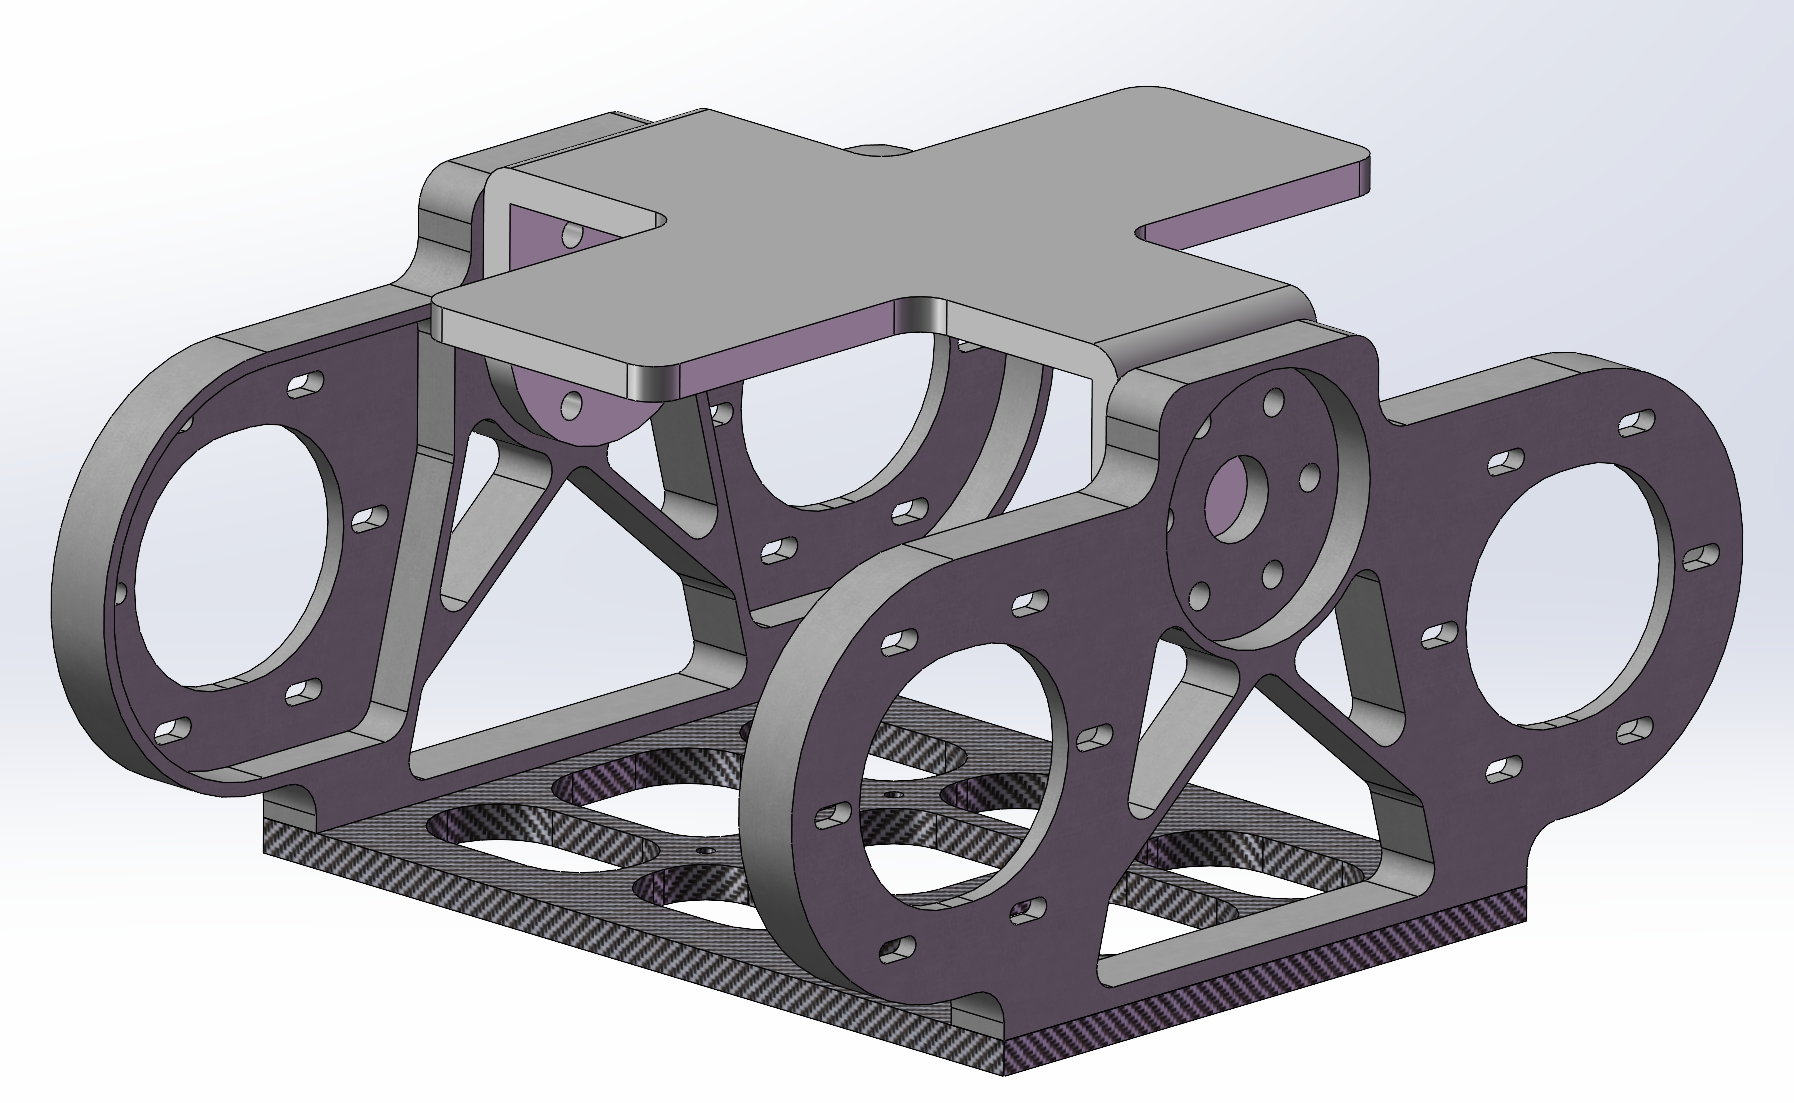
\includegraphics[width=0.6\textwidth]{figures/ch02/image4.png}
  \caption{躯干结构设计示意图}
  \label{fig:body-structure}
\end{figure}

主要承载板件优先采用碳纤维板材或 7075/6061 铝合金加工。碳纤维板材比刚度较高，适合用于侧板和连接板；铝合金更适合轴承座、电机座等需要较高加工精度的部位。电池架、线束固定件等非主要受力部件采用 3D 打印件，便于快速修改结构。

惯性测量单元尽量安装在靠近机体几何中心的位置，以减小局部振动和结构弹性对姿态测量的影响。电池和驱动器也尽量对称布置，避免左右腿支撑力出现明显静态偏差。

\section{传动系统设计}

传动系统负责把躯干附近电机的输出力矩传递到腿部连杆。设计时需控制传动回差和弹性变形，同时避免引入过多附加质量。本文传动部分包括髋关节嵌套轴系和链传动。

\subsection{髋关节轴系设计}

髋关节轴系采用嵌套式二级轴系，通过内外两层转动轴和两组轴承传递不同自由度的力矩。内轴系主要传递膝关节相关驱动力矩，外轴系支撑髋部连杆运动。该结构横向尺寸较小，适合布置在双腿之间的有限空间内。

\begin{figure}[H]
  \centering
  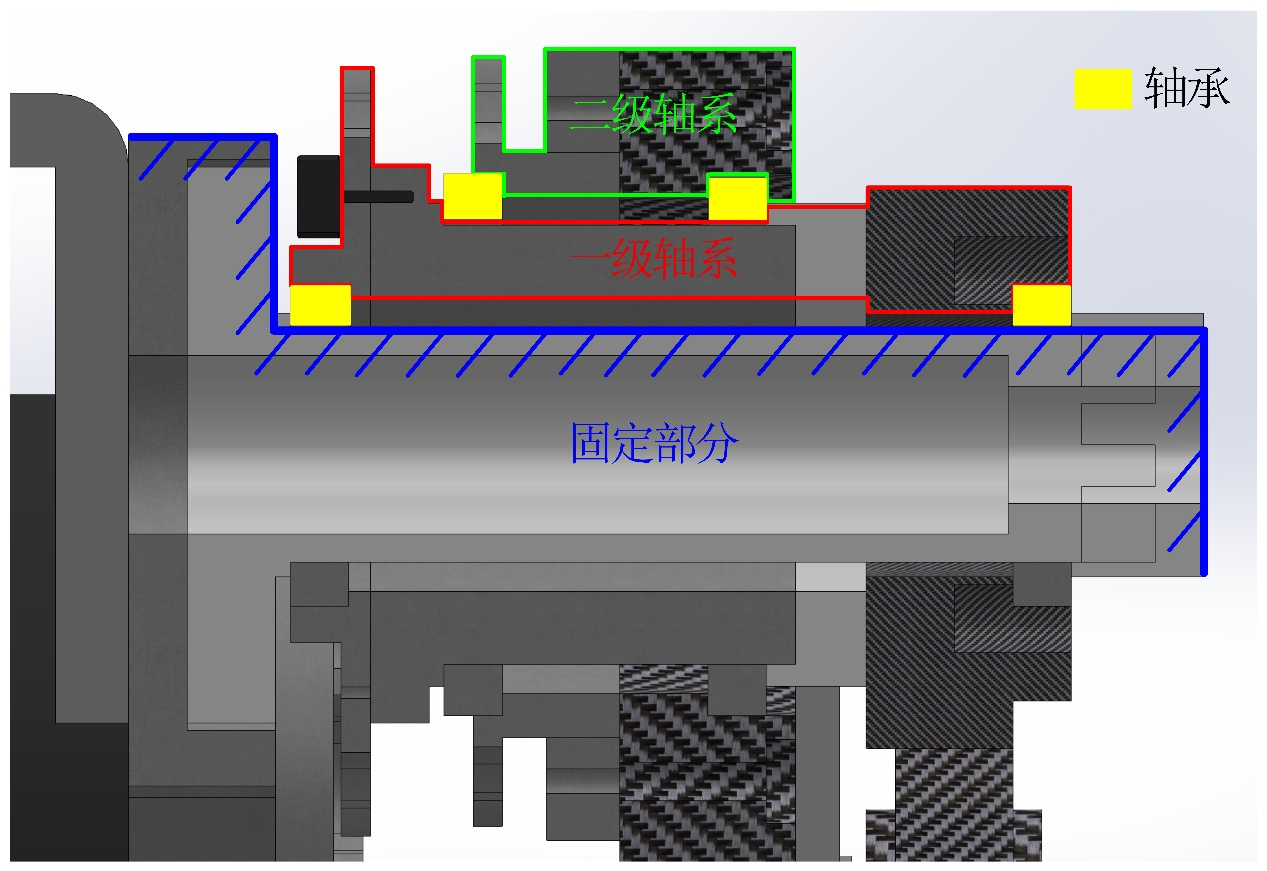
\includegraphics[width=0.8\textwidth]{figures/ch02/image5.jpeg}
  \caption{髋关节嵌套轴系结构示意图}
  \label{fig:hip-axis}
\end{figure}

与将电机直接安装在腿部远端相比，嵌套轴系配合后置电机可减小腿部摆动部件质量。该方案对装配精度和轴系同轴度要求更高，因此加工时需要保证轴承座定位精度，并通过预紧减小轴向间隙。

\subsection{链传动设计与校核}

腿部力矩传递采用 9 速自行车链条。与同步带相比，滚子链属于啮合传动，平均传动比更稳定，抗拉强度也更高；与常见工业链条相比，自行车链条宽度较小，有利于控制腿部横向尺寸。

在跳跃落地或快速伸腿工况下，链条会承受较大的瞬时拉力。以腿部电机说明书给出的峰值扭矩 $T_{\text{peak}} = 7\,\mathrm{N\cdot m}$、链轮等效直径 $d = 0.04907\,\mathrm{m}$ 估算，有效圆周力为

\begin{equation}
  F_t = \frac{2 T_{\text{peak}}}{d}
  = \frac{2 \times 7}{0.04907}
  \approx 285.3\,\mathrm{N}.
\end{equation}

主流 9 速自行车链条的最小破坏载荷通常可达到

\begin{equation}
  F_u \geq 8500\,\mathrm{N}.
\end{equation}

由此可得静强度安全系数

\begin{equation}
  S = \frac{F_u}{F_t}
  = \frac{8500}{285.3}
  \approx 29.79.
\end{equation}

即使考虑冲击载荷系数 $K_A \approx 1.5$，链条强度仍有余量。

\begin{figure}[H]
  \centering
  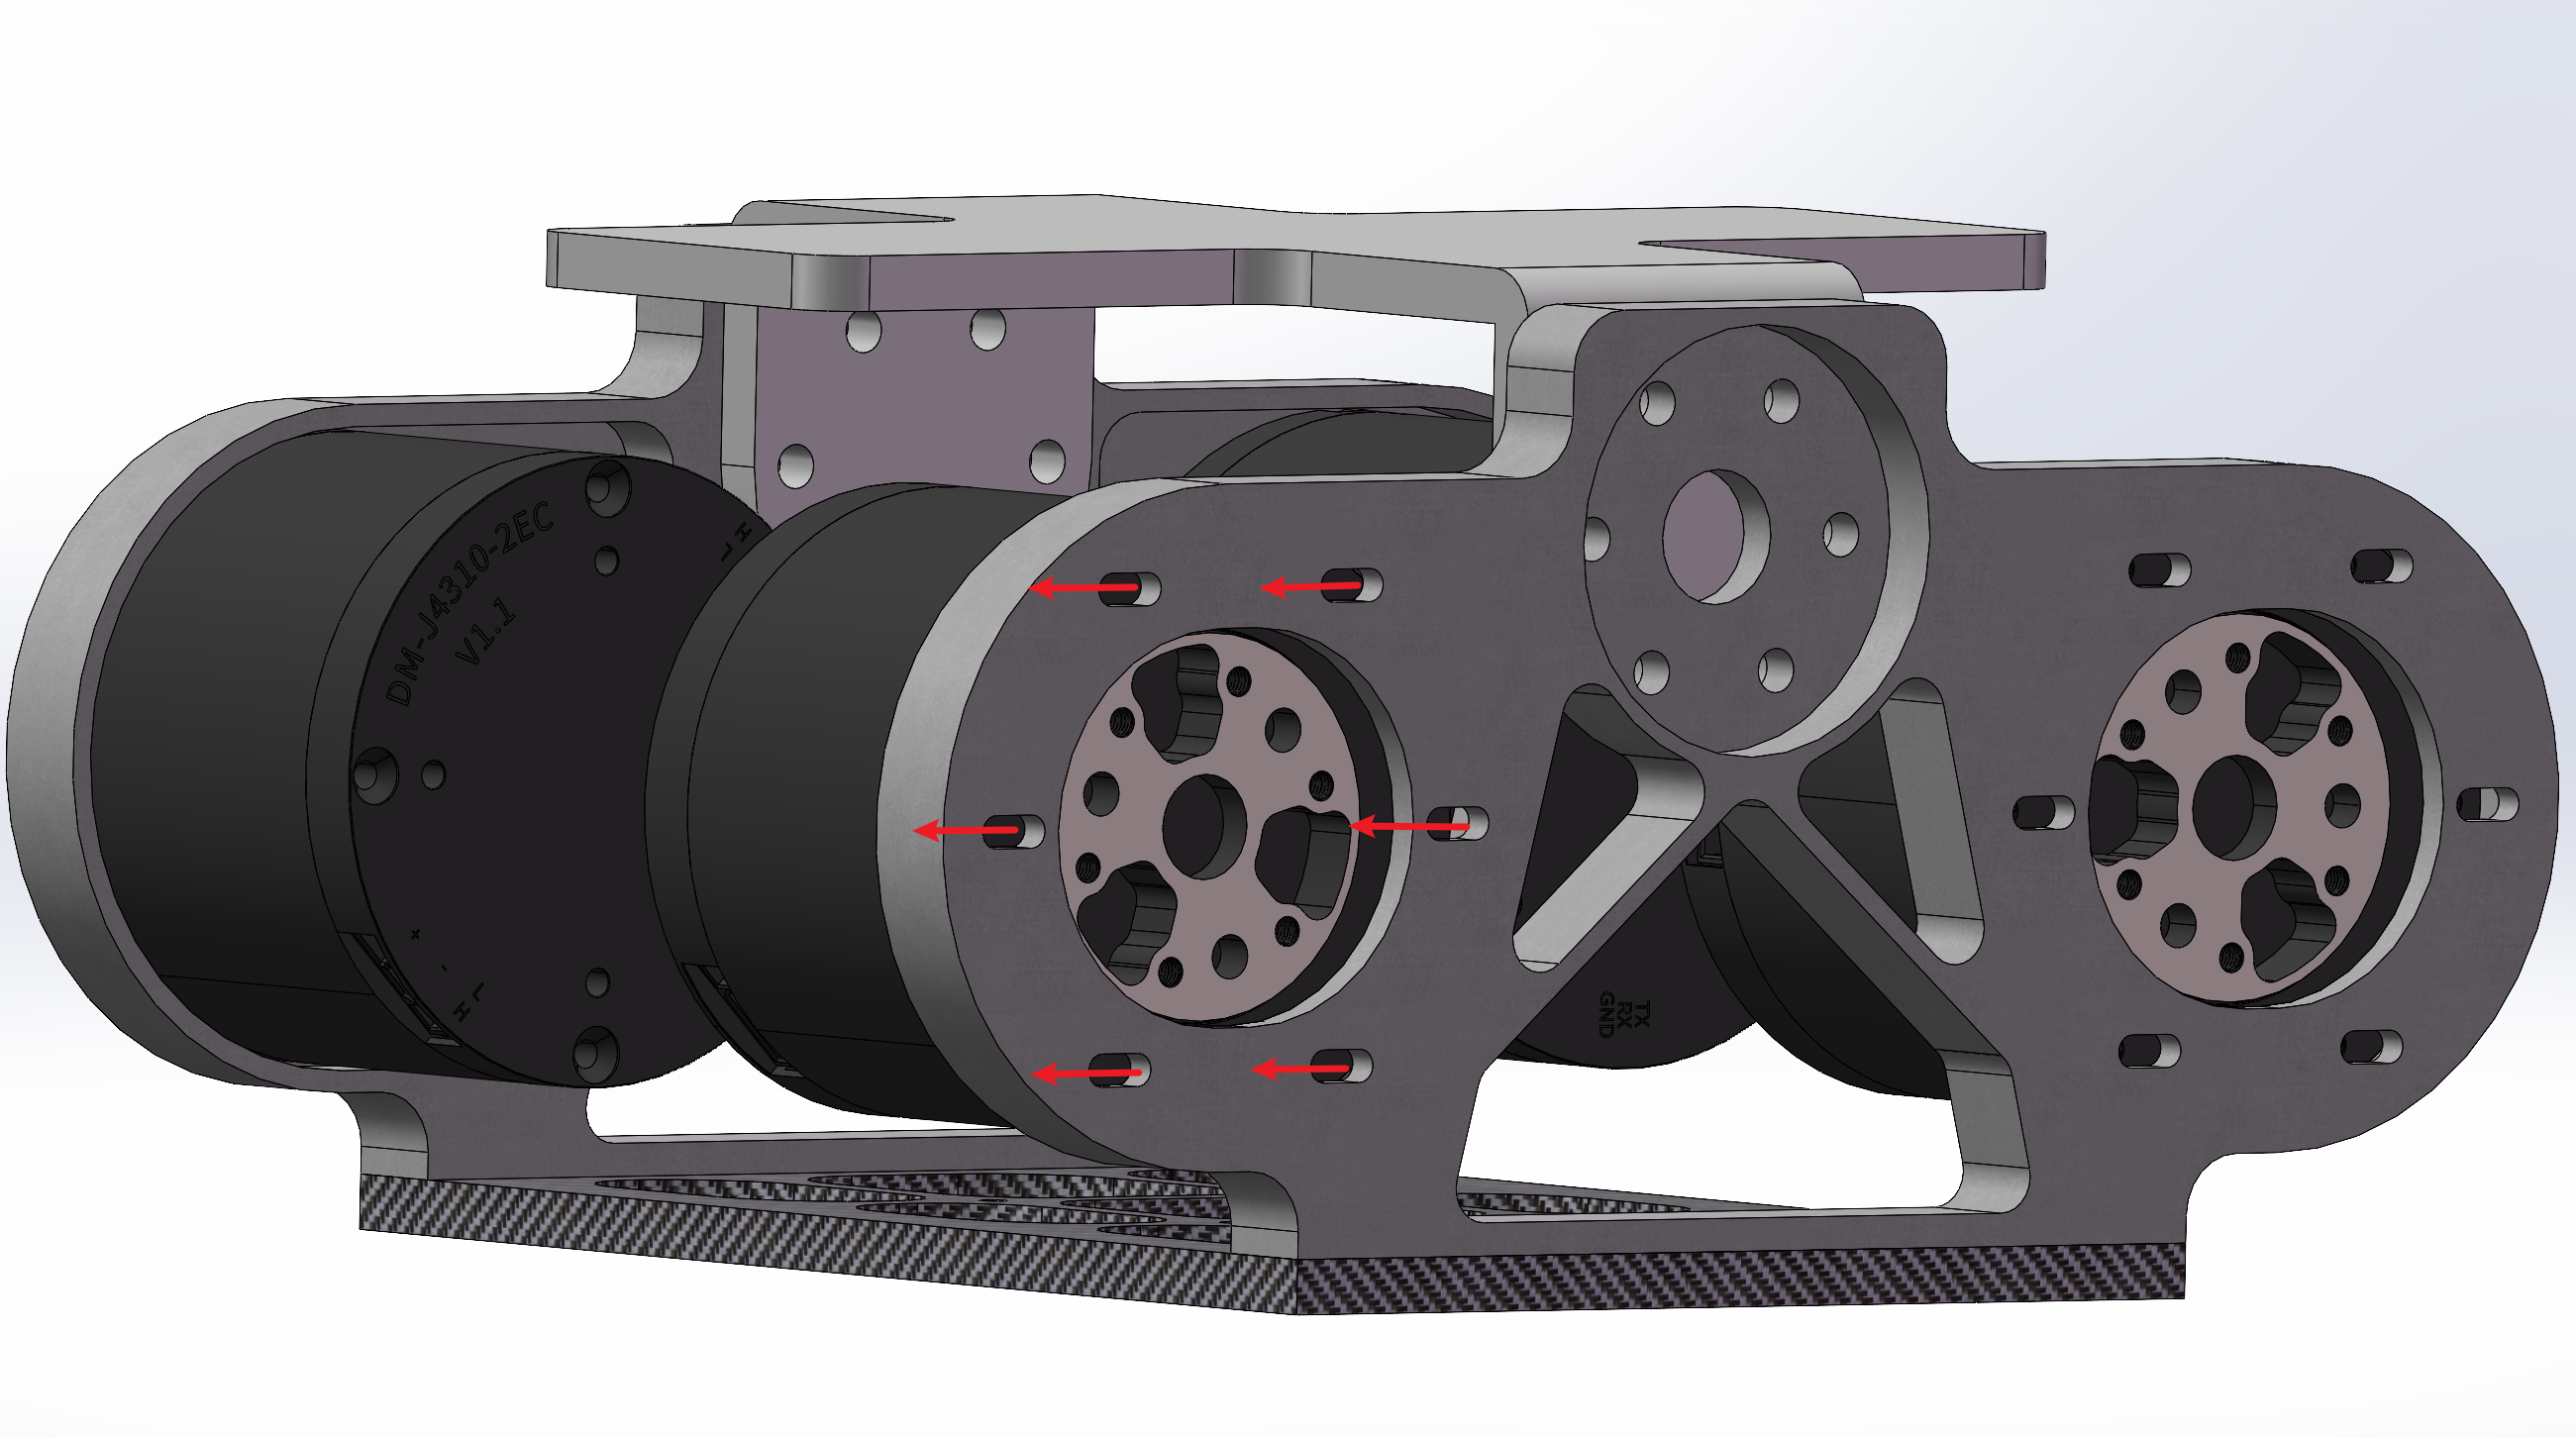
\includegraphics[width=0.8\textwidth]{figures/ch02/image6.png}
  \caption{髋关节连接板滑槽示意图}
  \label{fig:chain-drive}
\end{figure}

链条长期工作后会因销轴和套筒磨损而变长。链条过松会增大传动回差，影响倒立摆平衡控制，也会在冲击工况下增加脱链风险。为避免增加弹簧张紧臂或惰轮机构，本文通过改变中心距完成张紧：在髋关节连接板上将电机安装孔设计为水平滑槽，滑槽长度为 $7\,\mathrm{mm}$，允许电机定子沿水平方向进行约 $\pm 4\,\mathrm{mm}$ 的位置调整。这样不需要增加额外运动部件，维护时也比较直接。

\section{轮组系统设计}

轮组用于平地移动和差速转向。驱动轮直接集成在腿部末端，既是轮式模式下的支撑点，也是虚拟腿末端点。该布置省去了额外足端传动机构，可降低结构复杂度和质量。

\begin{figure}[H]
  \centering
  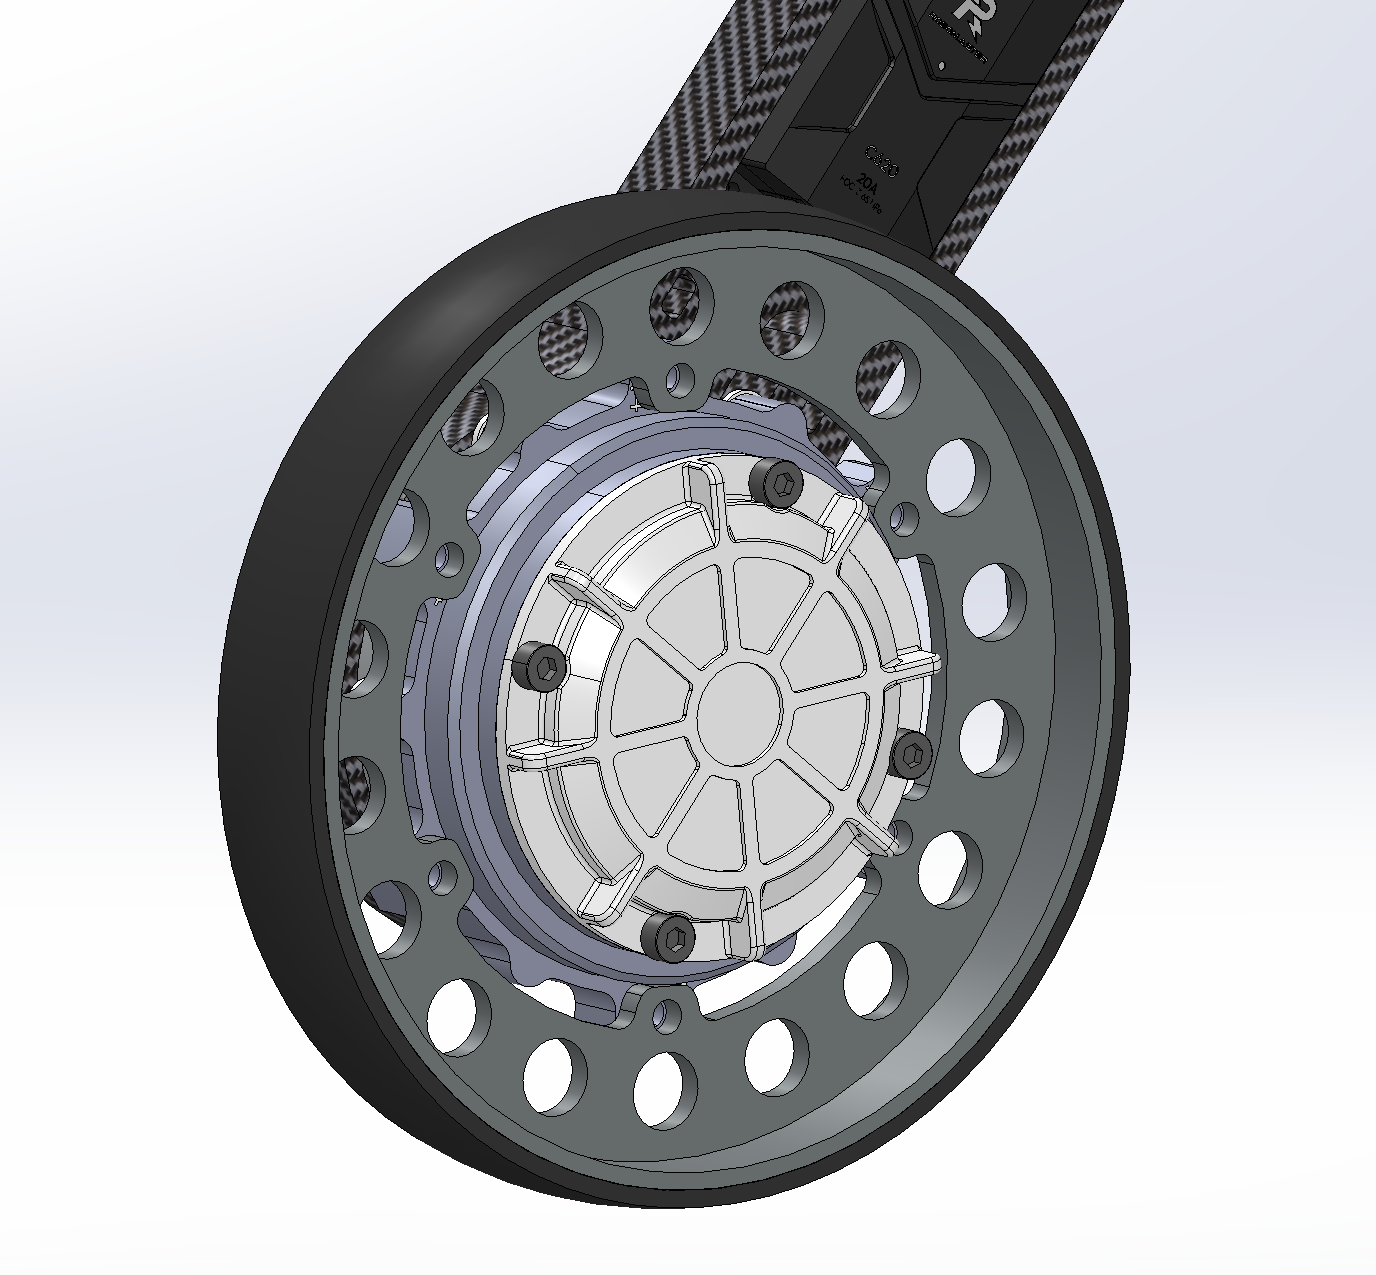
\includegraphics[width=0.5\textwidth]{figures/ch02/image9.png}
  \caption{足端轮组结构示意图}
  \label{fig:wheel-module}
\end{figure}

设轮子半径为 $r = 0.06\,\mathrm{m}$，根据最大移动速度指标 $v_{\max} \geq 2\,\mathrm{m/s}$，轮组所需角速度为

\begin{equation}
  \omega = \frac{v_{\max}}{r}
  = \frac{2}{0.06}
  \approx 33.3\,\mathrm{rad/s}
  \approx 318\,\mathrm{RPM}.
\end{equation}

若机器人在 $0.5\,\mathrm{s}$ 内由静止加速至 $2\,\mathrm{m/s}$，所需加速度为

\begin{equation}
  a = 4\,\mathrm{m/s^2}.
\end{equation}

当整机质量取 $M = 5\,\mathrm{kg}$、滚动阻力系数取 $\mu = 0.05$ 时，总牵引力需求为

\begin{equation}
  F_{\text{total}} = Ma + \mu Mg
  = 20 + 0.05 \times 5 \times 9.8
  = 22.45\,\mathrm{N}.
\end{equation}

对应轮组总扭矩为

\begin{equation}
  T_{\text{acc}} = F_{\text{total}} r
  = 22.45 \times 0.06
  \approx 1.35\,\mathrm{N\cdot m}.
\end{equation}

在爬坡工况下，若坡度取 $\alpha = 20^\circ$，重力沿坡面方向的分量为

\begin{equation}
  F_{\text{climb}} = Mg \sin \alpha
  = 5 \times 9.8 \times 0.342
  \approx 16.8\,\mathrm{N},
\end{equation}

对应爬坡扭矩为

\begin{equation}
  T_{\text{climb}} = F_{\text{climb}} r
  = 16.8 \times 0.06
  \approx 1.01\,\mathrm{N\cdot m}.
\end{equation}

双轮驱动时，单轮连续扭矩需求约为 $0.7 \sim 1.0\,\mathrm{N\cdot m}$。考虑加速、坡面扰动和控制裕度后，选用额定扭矩为 $2.5\,\mathrm{N\cdot m}$ 的减速轮毂电机。

\section{电机选型与校核}

执行器包括腿部关节电机和足端轮毂电机。腿部电机承担站立支撑、腿部伸缩和越障任务，轮毂电机承担轮式移动和差速转向任务。由于控制系统需要实时运行，电机需支持力矩控制，并具备足够的峰值扭矩。

\subsection{腿部关节电机}

腿部关节电机按跳跃起跳、落地缓冲和单腿支撑等工况估算。下文用跳跃起跳估算峰值扭矩，用半蹲支撑估算额定扭矩。

假设机器人需要实现原地跳跃，目标腾空高度为 $H_{\text{jump}} = 0.3\,\mathrm{m}$。根据能量守恒，机器人离地瞬间速度满足

\begin{equation}
  \frac{1}{2} M v_{\text{takeoff}}^2 = M g H_{\text{jump}},
\end{equation}

解得

\begin{equation}
  v_{\text{takeoff}} = \sqrt{2 g H_{\text{jump}}}
  \approx 2.42\,\mathrm{m/s}.
\end{equation}

若起跳阶段有效伸腿行程取 $h_{\text{acc}} = 0.15\,\mathrm{m}$，由动能定理可得地面对足端的平均反作用力

\begin{equation}
  F_{\text{ground}} =
  \frac{M g H_{\text{jump}}}{h_{\text{acc}}} + Mg
  = \frac{5 \times 9.8 \times 0.3}{0.15} + 49
  = 147\,\mathrm{N}.
\end{equation}

根据虚功原理，足端力与关节力矩满足 $\boldsymbol{\tau} = \boldsymbol{J}^{\mathsf{T}}\boldsymbol{F}$。在典型半蹲姿态下，设等效连杆长度为 $L_{\text{link}} \approx 0.15\,\mathrm{m}$，有效力臂系数取 0.7，则峰值关节力矩可估算为

\begin{equation}
  T_{\text{peak}} \approx
  F_{\text{ground}} L_{\text{link}} \times 0.7
  \approx 147 \times 0.15 \times 0.7
  \approx 15.4\,\mathrm{N\cdot m}.
\end{equation}

上述估算按较保守的工况取值。实际样机为双腿协同支撑，且每条腿由两个主动关节电机和闭环连杆机构共同承担负载，单电机峰值需求会低于该估算。综合质量、体积和控制接口，腿部关节驱动器选用额定扭矩 $3\,\mathrm{N\cdot m}$、峰值扭矩 $7\,\mathrm{N\cdot m}$ 的无刷减速电机。该电机支持 MIT、速度和位置控制模式，满足站立平衡和腿部快速调节需求。

\begin{figure}[H]
  \centering
  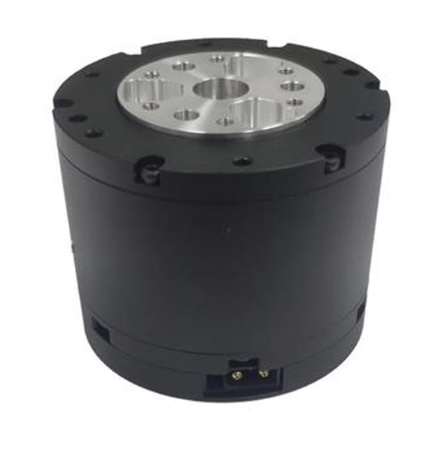
\includegraphics[width=0.4\textwidth]{figures/ch02/image7.jpg}
  \caption{腿部关节驱动电机}
  \label{fig:leg-motor}
\end{figure}

\begin{table}[H]
  \centering
  \caption{腿部关节驱动电机关键参数}
  \label{tab:leg-motor-parameters}
  \begin{tabular}{lcc}
    \toprule
    参数 & 数值 & 说明 \\
    \midrule
    额定扭矩 & $3\,\mathrm{N\cdot m}$ & 连续输出扭矩 \\
    峰值扭矩 & $7\,\mathrm{N\cdot m}$ & 短时输出扭矩 \\
    额定转速 & $120\,\mathrm{r/min}$ & 减速后输出转速 \\
    空载最大转速 & $200\,\mathrm{r/min}$ & 空载工况 \\
    减速比 & $10:1$ & 内置减速机构 \\
    电机质量 & 约 $300\,\mathrm{g}$ & 单个电机 \\
    \bottomrule
  \end{tabular}
\end{table}

对于静态或准静态半蹲支撑工况，若按单腿支撑整机重量进行保守估算，有

\begin{equation}
  T_{\text{rated}} =
  Mg L_{\text{link}} \sin 45^\circ
  \approx 5 \times 9.8 \times 0.15 \times 0.707
  \approx 5.2\,\mathrm{N\cdot m}.
\end{equation}

双腿支撑时，单腿持续负载约减半，即约为 $2.6\,\mathrm{N\cdot m}$。所选电机额定扭矩为 $3\,\mathrm{N\cdot m}$，可覆盖该需求，并为姿态调节和小扰动恢复留出余量。

\subsection{轮毂电机}

轮毂电机按第 2.5 节的速度、加速和爬坡需求选型。本文选用额定扭矩为 $2.46\,\mathrm{N\cdot m}$ 的 M3508 减速轮毂电机，并将其直接布置在足端轮组内部。该方案省去额外传动链，轮系角度和速度也可直接用于估计前进位移与速度。

\begin{figure}[H]
  \centering
  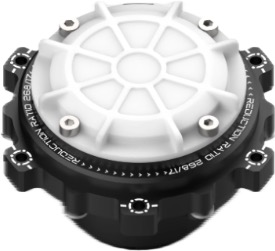
\includegraphics[width=0.3\textwidth]{figures/ch02/image8_safe.jpg}
  \caption{足端轮毂电机}
  \label{fig:wheel-motor}
\end{figure}

\begin{table}[H]
  \centering
  \caption{足端轮毂电机关键参数}
  \label{tab:wheel-motor-parameters}
  \begin{tabular}{lcc}
    \toprule
    参数 & 数值 & 说明 \\
    \midrule
    额定扭矩 & $2.46\,\mathrm{N\cdot m}$ & 减速箱输出端 \\
    堵转扭矩 & $3.69\,\mathrm{N\cdot m}$ & 短时极限输出 \\
    额定转速 & $571\,\mathrm{r/min}$ & 减速后输出转速 \\
    空载转速 & $587\,\mathrm{r/min}$ & 空载工况 \\
    最大效率 & $70\%$ & 电机效率 \\
    电机质量 & $336.4\,\mathrm{g}$ & 单个电机 \\
    \bottomrule
  \end{tabular}
\end{table}

根据前述计算，双轮驱动下单轮连续扭矩需求约为 $0.7 \sim 1.0\,\mathrm{N\cdot m}$，所选轮毂电机额定扭矩为 $2.46\,\mathrm{N\cdot m}$，可满足平地加速和一定坡度爬升需求。直接驱动形式还能减少传动回差，使轮系状态估计更简单。

\section{本章小结}

本章完成了样机机械结构设计。根据平衡移动、越障、轻量化和嵌入式实时控制需求，确定了整机质量、自由度、移动速度和越障高度等指标；设计了带闭环支链的混合式腿部机构，并通过连杆尺寸和工作空间分析验证其伸缩范围；给出了躯干、髋关节轴系、链传动和足端轮组方案，并对链条强度、腿部关节电机和轮毂电机进行了估算校核。

最终样机采用躯干集中承载、混合式腿部支撑调节、足端轮组驱动移动的结构。第三章将基于该结构建立运动学和动力学模型。

\chapter{机器人运动学与动力学建模}\label{chap:model}

本章先把左右腿等效为可伸缩虚拟杆，建立二维多刚体模型；再针对第二章的混合式闭环连杆机构，给出闭环运动学和任务空间到关节空间的力矩映射；最后将原始广义坐标模型线性化，得到 LQR 控制器所需的状态空间表达式。

\section{建模与基本假设}

若直接用全部连杆和关节变量建立三维模型，模型精度会更高，但维度较大，约束关系也更复杂，不适合直接放入嵌入式控制器中实时计算。结合本文控制系统的规模，本章模型需要完成以下工作：

\begin{enumerate}
  \item 建立二维多刚体模型，描述前进、腿长变化、腿摆和机体俯仰之间的耦合关系；
  \item 给出轮系转角、腿部摆角与控制器状态变量之间的运动学映射；
  \item 推导 LQR 设计所需的线性化状态空间表达式；
  \item 建立闭环腿部机构的任务空间映射，将 VMC 输出转换为关节力矩命令。
\end{enumerate}

建模时保留两套变量：一套是原始广义坐标，用于构造运动控制器的独立坐标模型；另一套是虚拟腿任务空间变量，用于描述腿部支撑和摆动。原始广义坐标取为
\begin{equation}
  \boldsymbol{q} =
  \begin{bmatrix}
    \theta_{wl} & \theta_{wr} & \theta_{ll} & \theta_{lr} & \theta_b
  \end{bmatrix}^{\mathsf{T}}
  \label{eq:generalized-coordinate-origin}
\end{equation}
其中，$\theta_{wl}$ 和 $\theta_{wr}$ 分别表示左、右轮转角，$\theta_{ll}$ 和 $\theta_{lr}$ 分别表示左、右虚拟腿摆角，$\theta_b$ 表示机体俯仰角。与之对应的控制输入记为
\begin{equation}
  \boldsymbol{u} =
  \begin{bmatrix}
    T_{lw,l} & T_{lw,r} & T_{bl,l} & T_{bl,r}
  \end{bmatrix}^{\mathsf{T}}
  \label{eq:input-origin}
\end{equation}
其中，$T_{lw,l}$、$T_{lw,r}$ 为左右轮电机输出转矩，$T_{bl,l}$、$T_{bl,r}$ 为左右腿驱动关节输出转矩。

混合式闭环腿部机构的关节变量耦合较强，直接在关节空间设计支撑和摆动控制并不直观。这里按虚功等效思想，将单腿抽象为连接髋关节与轮轴中心的可伸缩虚拟杆。虚拟杆长度表示腿部伸缩状态，虚拟杆相对竖直方向的转角表示腿部摆动状态。腿部任务空间控制量定义为
\begin{equation}
  \boldsymbol{F}_v =
  \begin{bmatrix}
    F_l \\
    T_\theta
  \end{bmatrix}
  \label{eq:virtual-force-def}
\end{equation}
其中，$F_l$ 为沿虚拟杆方向的轴向虚拟力，用于调节支撑力与腿长；$T_\theta$ 为绕髋关节的虚拟转矩，用于调节腿部摆动姿态。若采用线性弹簧阻尼形式构造虚拟元件，则有
\begin{equation}
  \left\{
    \begin{aligned}
      F_l      &= K_l (l_d - l) + D_l (\dot{l}_d - \dot{l}) \\
      T_\theta &= K_\theta (\theta_{ld} - \theta_l) + D_\theta (\dot{\theta}_{ld} - \dot{\theta}_l)
    \end{aligned}
  \right.
  \label{eq:vmc-law}
\end{equation}
式中，$l_d$ 与 $\theta_{ld}$ 分别为虚拟腿长和平均虚拟腿摆角的期望值；$K_l$、$D_l$、$K_\theta$ 与 $D_\theta$ 分别为对应方向的虚拟刚度系数与虚拟阻尼系数。这样，腿部控制可先在任务空间中给出支撑力和摆动转矩，再映射到实际关节力矩。

为控制模型复杂度，并使模型与后续分层控制器的职责划分一致，本文作如下假设：
\begin{enumerate}
  \item 将机器人简化为机体、左腿、右腿、左驱动轮和右驱动轮五部分组成的刚体系统，忽略连杆柔性变形、轴承间隙和摩擦损失对主要动力学行为的影响；
  \item 忽略腿部闭环连杆机构内部运动产生的附加动力学效应，包括连杆姿态变化、腿长变化和等效惯量变化带来的高阶影响，任一时刻均将腿部视为由当前腿长参数确定的刚体；
  \item 忽略腿部与机体位形变化对驱动轮轴向转动惯量的影响，轮组惯量在建模和控制器设计中取为常值；
  \item 驱动轮与地面满足纯滚动约束，不考虑轮胎侧偏、纵向打滑和接触点弹性变形，后续实验中再结合离地和打滑检测对该假设进行修正；
  \item 机体滚转角由腿部控制器单独补偿，在整机主动力学分析中取滚转角及其一、二阶导数为零，即 $\gamma=\dot{\gamma}=\ddot{\gamma}=0$；
  \item 腿部支撑力由腿部控制器调节，在整机主动力学分析中假设左右腿支撑力保持相等，忽略侧向惯性力矩对运动模型的影响。
\end{enumerate}

上述假设将建模重点集中在前进、俯仰、腿长和腿摆等主要自由度上，同时把滚转补偿、支撑力分配和轮地异常接触留给第四章控制器及第五章实验验证处理。

\section{坐标系与符号定义}

机器人简化刚体模型及坐标系如\figref{fig:model-coordinate} 所示。取地面惯性坐标系 $\Sigma_I = \{O_I, s, h\}$，其中 $s$ 轴沿机器人前进方向，$h$ 轴竖直向上。轮轴中心记为点 $W$，髋关节记为点 $H$，机体质心记为点 $B$。等效虚拟腿长度记为 $l$，平均虚拟腿摆角记为 $\theta_l$，机体俯仰角记为 $\theta_b$，轮半径记为 $R_w$，轮轴中心水平位移记为 $s$。系统偏航角记为 $\phi$，仅在后续状态空间变量构造中使用。

\begin{figure}[H]
  \centering
  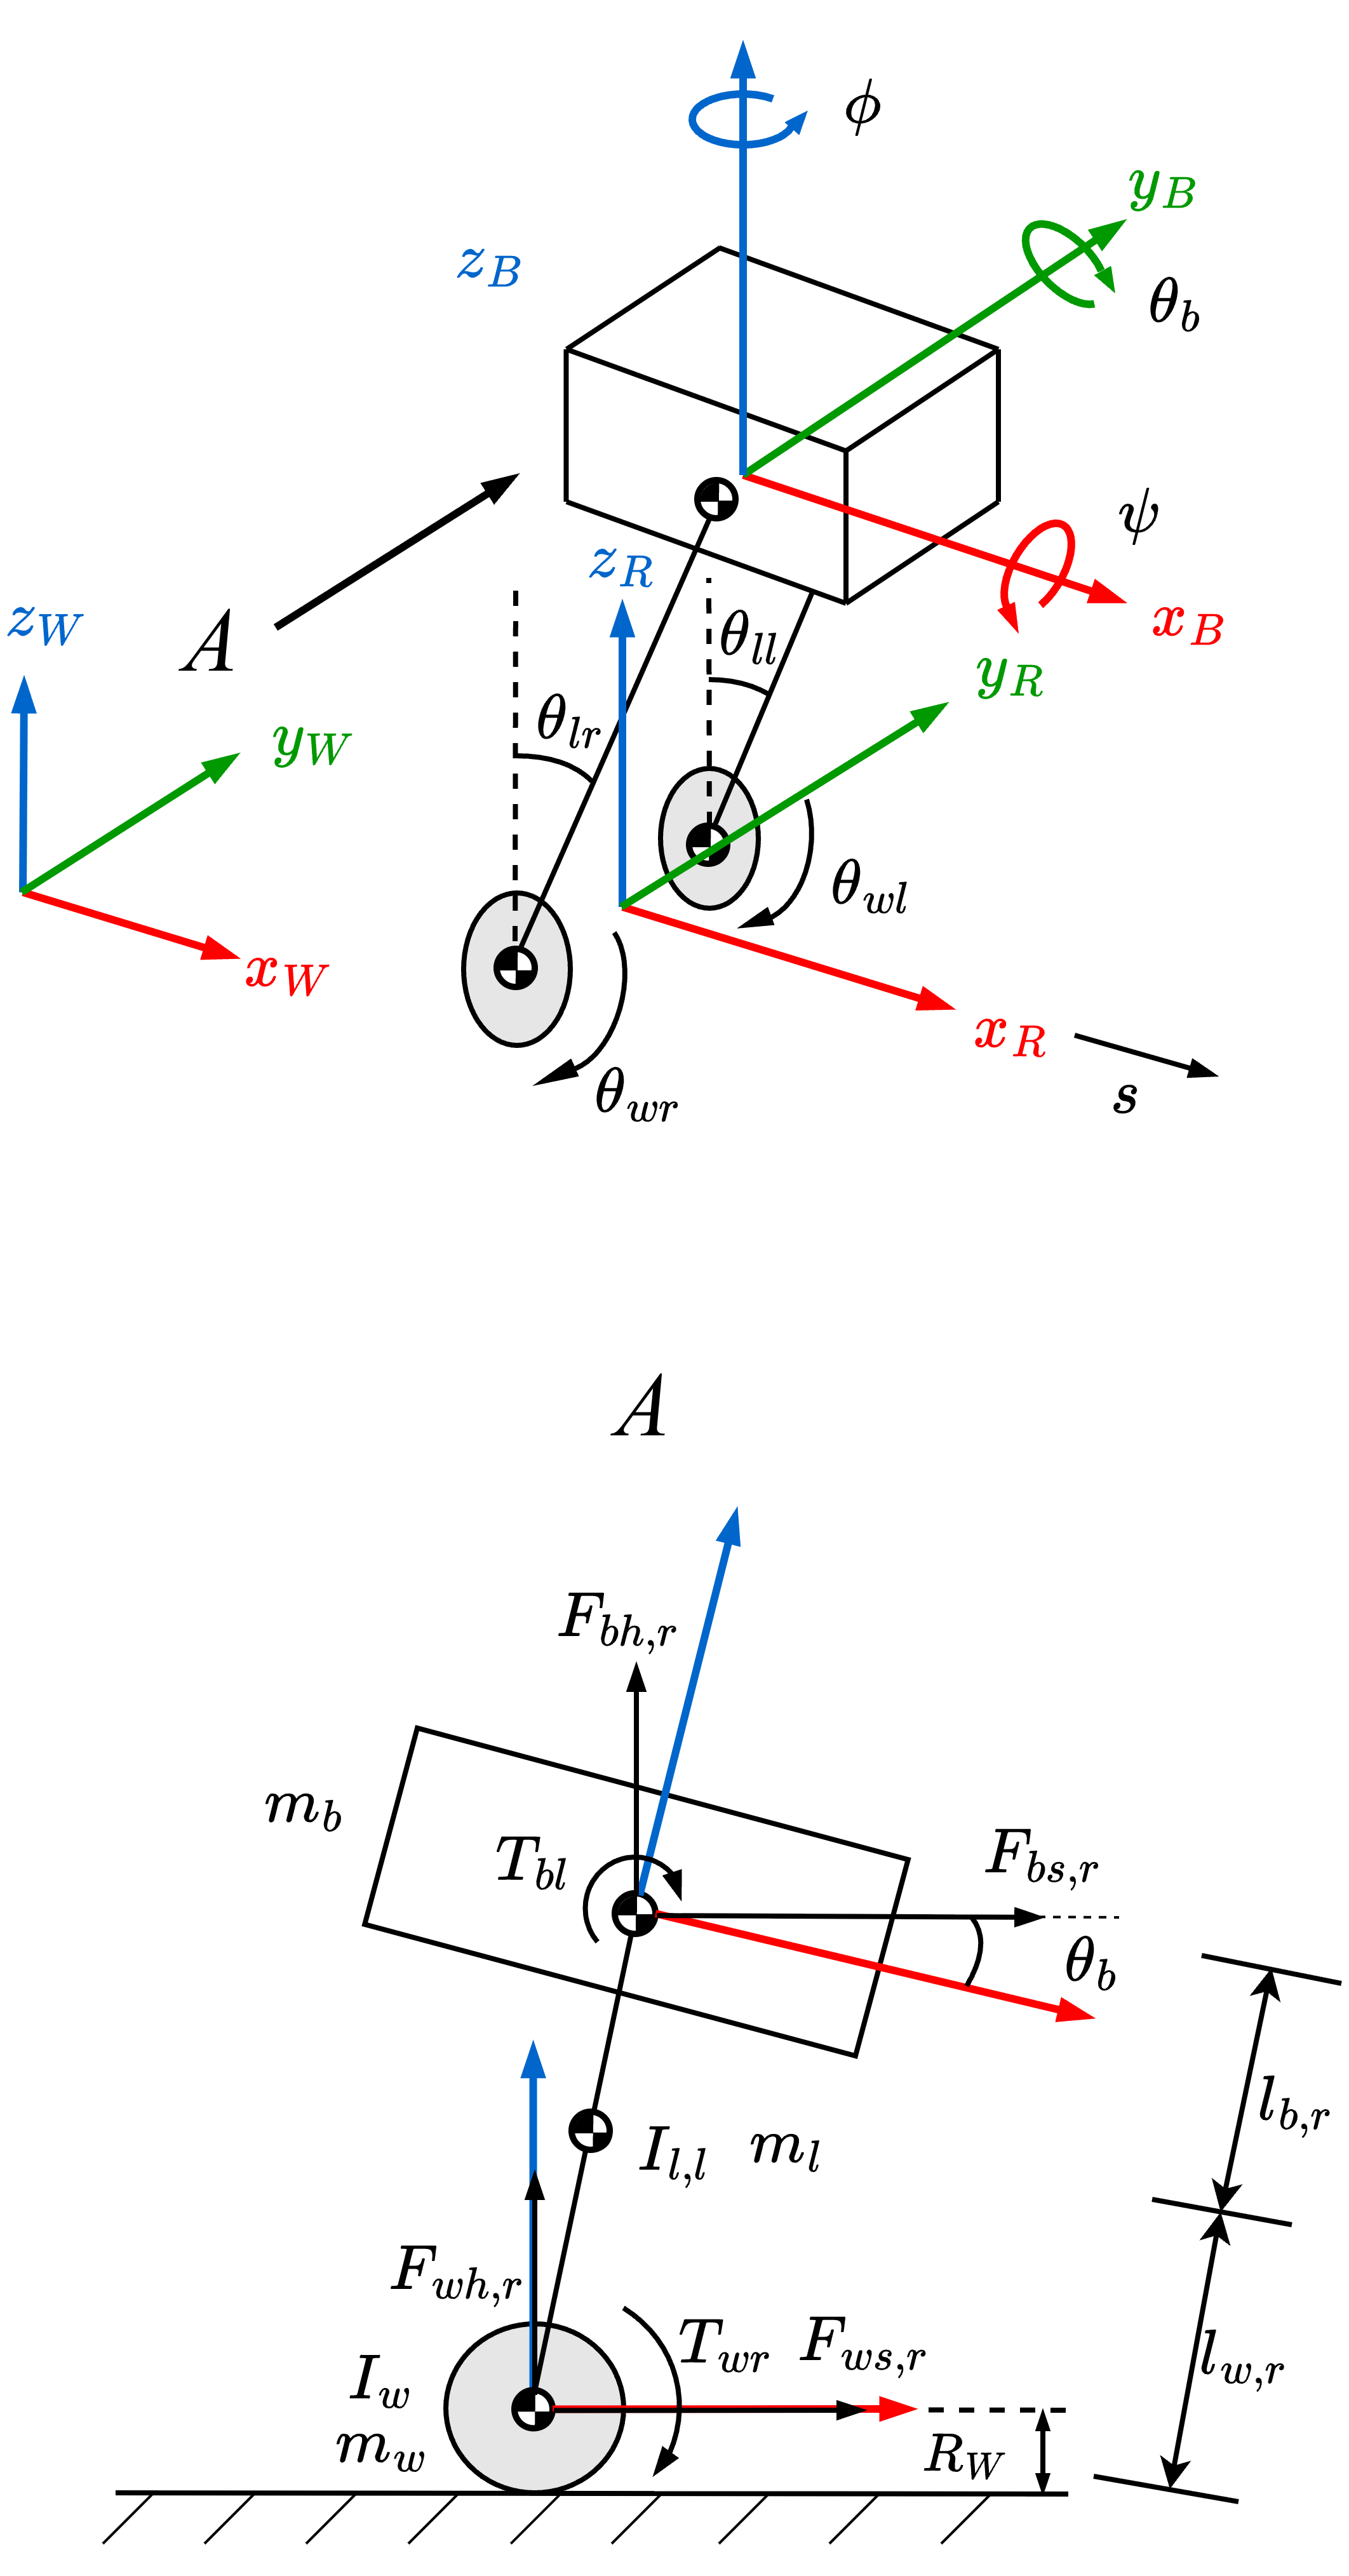
\includegraphics[width=0.48\textwidth]{figures/ch03/robot.png}
  \caption{机器人简化刚体模型及坐标系定义}
  \label{fig:model-coordinate}
\end{figure}

本章主要符号列于\tabref{tab:model-symbols}。

\begin{table}[H]
  \centering
  \caption{模型主要符号定义}\label{tab:model-symbols}
  \renewcommand{\arraystretch}{1.25}
  \begin{tabular}{@{}clp{8.2cm}@{}}
    \toprule
    符号 & 单位 & 含义 \\
    \midrule
    $\theta_{wl} \theta_{wr}$ & rad & 左、右轮转角 \\
    $\theta_{ll} \theta_{lr}$ & rad & 左、右虚拟腿摆角 \\
    $\theta_b$ & rad & 机体俯仰角 \\
    $s$ & m & 轮轴中心在惯性坐标系中的水平位移 \\
    $\phi$ & rad & 机器人偏航角，由左右轮差动及腿部横摆共同决定 \\
    $R_w$ & m & 驱动轮半径 \\
    $R_l$ & m & 半轮距，即机器人纵向中面到单侧轮接地点的距离 \\
    $l_l, l_r$ & m & 左、右腿等效长度参数\\
    $l_b$ & m & 髋关节至机体质心的距离 \\
    $m_w, m_l, m_b$ & kg & 分别表示轮组、虚拟腿等效构件和机体的质量 \\
    $I_w, I_i, I_b$ & kg$\cdot$m$^2$ & 分别表示轮组、虚拟腿等效构件和机体绕质心的转动惯量 \\
    $F_l$ & N & 沿虚拟腿方向的轴向虚拟力 \\
    $T_\theta$ & N$\cdot$m & 绕髋关节作用于虚拟腿的摆动虚拟转矩 \\
    $T_{lw,l} T_{lw,r}$ & N$\cdot$m & 左、右轮电机输出转矩 \\
    $T_{bl,l} T_{bl,r}$ & N$\cdot$m & 左、右腿驱动关节输出转矩 \\
    $\boldsymbol{q}$ & -- & 原始广义坐标向量，取 $\boldsymbol{q} = [\theta_{wl}\, \theta_{wr}\, \theta_{ll}\, \theta_{lr}\, \theta_b]^\mathsf{T}$ \\
    $\boldsymbol{q}_v$ & -- & 二维等效模型广义坐标向量，取 $\boldsymbol{q}_v = [s,\, l,\, \theta_l,\, \theta_b]^\mathsf{T}$ \\
    \bottomrule
  \end{tabular}
\end{table}

\section{多刚体系统运动学建模}

本节建立关键点位置、速度与广义坐标之间的关系。根据\figref{fig:model-coordinate}，分别写出轮轴中心、虚拟腿等效质心、髋关节和机体质心的位置，并由此得到速度和雅可比矩阵。

为避免正文被展开式打断，本节只保留后续控制设计直接使用的运动学关系；左右腿完整位置、速度和加速度方程见附录 \ref{app:kinematics}.

在平面模型下，轮轴中心、虚拟腿等效质心、髋关节和机体质心在惯性坐标系中的位置分别为
\begin{equation}
  \boldsymbol{p}_W =
  \begin{bmatrix}
    s \\
    R_w
  \end{bmatrix}
  \label{eq:w-pos}
\end{equation}
\begin{equation}
  \boldsymbol{p}_L =
  \begin{bmatrix}
    s + \dfrac{l}{2}\sin\theta_l \\
    R_w + \dfrac{l}{2}\cos\theta_l
  \end{bmatrix}
  \label{eq:l-pos}
\end{equation}
\begin{equation}
  \boldsymbol{p}_H =
  \begin{bmatrix}
    s + l\sin\theta_l \\
    R_w + l\cos\theta_l
  \end{bmatrix}
  \label{eq:h-pos}
\end{equation}
\begin{equation}
  \boldsymbol{p}_B =
  \begin{bmatrix}
    s + l\sin\theta_l + l_b\sin\theta_b \\
    R_w + l\cos\theta_l + l_b\cos\theta_b
  \end{bmatrix}.
  \label{eq:b-pos}
\end{equation}
式中，$\boldsymbol{p}_L$、$\boldsymbol{p}_H$ 和 $\boldsymbol{p}_B$ 分别表示虚拟腿等效构件质心、髋关节和机体质心的位置。

由左右轮纯滚动约束可得
\begin{equation}
  s = \frac{R_w}{2}\left(\theta_{wl} + \theta_{wr}\right),\qquad
  \dot{s} = \frac{R_w}{2}\left(\dot{\theta}_{wl} + \dot{\theta}_{wr}\right),\qquad
  \ddot{s} = \frac{R_w}{2}\left(\ddot{\theta}_{wl} + \ddot{\theta}_{wr}\right).
  \label{eq:rolling-constraint}
\end{equation}
\eqref{eq:rolling-constraint} 给出了轮系转角与前进位移之间的几何关系。偏航角不是平面模型中的独立广义坐标，其表达将在第 \ref{sec:state-space-model} 节通过运动学映射引入。

对\eqref{eq:l-pos} 和\eqref{eq:b-pos} 分别对时间求导，可得虚拟腿等效质心和机体质心的速度表达式
\begin{equation}
  \dot{\boldsymbol{p}}_L =
  \begin{bmatrix}
    \dot{s} + \dfrac{\dot{l}}{2}\sin\theta_l + \dfrac{l\dot{\theta}_l}{2}\cos\theta_l \\
    \dfrac{\dot{l}}{2}\cos\theta_l - \dfrac{l\dot{\theta}_l}{2}\sin\theta_l
  \end{bmatrix}
  \label{eq:l-vel}
\end{equation}
\begin{equation}
  \dot{\boldsymbol{p}}_B =
  \begin{bmatrix}
    \dot{s} + \dot{l}\sin\theta_l + l\dot{\theta}_l\cos\theta_l + l_b\dot{\theta}_b\cos\theta_b \\
    \dot{l}\cos\theta_l - l\dot{\theta}_l\sin\theta_l - l_b\dot{\theta}_b\sin\theta_b
  \end{bmatrix}.
  \label{eq:b-vel}
\end{equation}

将\eqref{eq:b-pos} 写成关于等效广义坐标 $\boldsymbol{q}_v$ 的函数形式 $\boldsymbol{p}_B = \boldsymbol{p}_B(\boldsymbol{q}_v)$，则机体质心速度可进一步表示为
\begin{equation}
  \dot{\boldsymbol{p}}_B = \boldsymbol{J}_B(\boldsymbol{q}_v)\dot{\boldsymbol{q}}_v,
  \label{eq:body-jacobian}
\end{equation}
其中，
\begin{equation}
  \boldsymbol{J}_B(\boldsymbol{q}_v) =
  \begin{bmatrix}
    1 & \sin\theta_l & l\cos\theta_l & l_b\cos\theta_b \\
    0 & \cos\theta_l & -l\sin\theta_l & -l_b\sin\theta_b
  \end{bmatrix}.
  \label{eq:body-jacobian-matrix}
\end{equation}

由\eqref{eq:l-vel} 至\eqref{eq:body-jacobian-matrix} 可知，虚拟腿长度 $l$ 与平均腿摆角 $\theta_l$ 不仅决定整机几何构型，也影响机体平动与俯仰运动之间的耦合关系。

\section{多刚体系统动力学建模}

动力学模型用于描述驱动力矩、虚拟腿支撑力和重力作用下的运动响应。平面等效模型由轮组、虚拟腿等效构件和机体三部分组成，下面采用拉格朗日方法建立动力学方程。

系统总动能可写为
\begin{equation}
  T = T_w + T_l + T_b,
  \label{eq:kinetic-total}
\end{equation}
其中
\begin{equation}
  T_w = \frac{1}{2}m_w\dot{s}^2 + \frac{1}{2}I_w\left(\frac{\dot{s}}{R_w}\right)^2,
  \label{eq:kinetic-wheel}
\end{equation}
\begin{equation}
  T_l = \frac{1}{2}m_l \dot{\boldsymbol{p}}_L^\mathsf{T}\dot{\boldsymbol{p}}_L + \frac{1}{2}I_i\dot{\theta}_l^2,
  \label{eq:kinetic-leg}
\end{equation}
\begin{equation}
  T_b = \frac{1}{2}m_b \dot{\boldsymbol{p}}_B^\mathsf{T}\dot{\boldsymbol{p}}_B + \frac{1}{2}I_b\dot{\theta}_b^2.
  \label{eq:kinetic-body}
\end{equation}

取地面为势能零位，则系统总势能为
\begin{equation}
  V = m_l g\left(R_w + \frac{l}{2}\cos\theta_l\right) + m_b g\left(R_w + l\cos\theta_l + l_b\cos\theta_b\right),
  \label{eq:potential-total}
\end{equation}
式中，轮组重力势能为常数项，对动力学方程无影响，因此未单独列出。

引入平面等效广义坐标
\begin{equation}
  \boldsymbol{q}_v =
  \begin{bmatrix}
    s & l & \theta_l & \theta_b
  \end{bmatrix}^{\mathsf{T}}
  \label{eq:generalized-coordinate-v}
\end{equation}
并定义拉格朗日函数
\begin{equation}
  \mathcal{L} = T - V.
  \label{eq:lagrangian}
\end{equation}
则系统满足
\begin{equation}
  \frac{\mathrm{d}}{\mathrm{d}t}\left(\frac{\partial \mathcal{L}}{\partial \dot{\boldsymbol{q}}_v}\right)
  -
  \frac{\partial \mathcal{L}}{\partial \boldsymbol{q}_v}
  = \boldsymbol{Q}_v,
  \label{eq:lagrange-equation}
\end{equation}
其中广义力向量取为
\begin{equation}
  \boldsymbol{Q}_v =
  \begin{bmatrix}
    \dfrac{T_{lw,l} + T_{lw,r}}{2R_w} \\
    F_l \\
    T_\theta \\
    0
  \end{bmatrix}.
  \label{eq:generalized-force}
\end{equation}
式中，第一个分量为左右轮驱动转矩在前进方向上的等效广义力，第二、三项分别对应 VMC 作用下的虚拟腿轴向力与摆动虚拟转矩。机体俯仰自由度不直接受驱动，因此第四项为零。

将\eqref{eq:kinetic-total} 至\eqref{eq:generalized-force} 代入\eqref{eq:lagrange-equation}，可得机器人平面等效模型的动力学方程
\begin{equation}
  \boldsymbol{M}_v(\boldsymbol{q}_v)\ddot{\boldsymbol{q}}_v
  +
  \boldsymbol{C}_v(\boldsymbol{q}_v, \dot{\boldsymbol{q}}_v)\dot{\boldsymbol{q}}_v
  +
  \boldsymbol{G}_v(\boldsymbol{q}_v)
  =
  \boldsymbol{B}_v\boldsymbol{u}_v,
  \label{eq:dynamics-compact}
\end{equation}
其中，
\begin{equation}
  \boldsymbol{u}_v =
  \begin{bmatrix}
    \dfrac{T_{lw,l} + T_{lw,r}}{2} & F_l & T_\theta
  \end{bmatrix}^{\mathsf{T}}\qquad
  \boldsymbol{B}_v =
  \begin{bmatrix}
    1/R_w & 0 & 0 \\
    0 & 1 & 0 \\
    0 & 0 & 1 \\
    0 & 0 & 0
  \end{bmatrix}.
  \label{eq:input-matrix}
\end{equation}

系统质量矩阵 $\boldsymbol{M}_v(\boldsymbol{q}_v)$ 具体为
\begin{equation}
\resizebox{\textwidth}{!}{$
  \boldsymbol{M}_v(\boldsymbol{q}_v) =
  \begin{bmatrix}
    m_w + m_l + m_b + I_w/R_w^2 &
    \left(\dfrac{m_l}{2} + m_b\right)\sin\theta_l &
    \left(\dfrac{m_l}{2} + m_b\right)l\cos\theta_l &
    m_b l_b \cos\theta_b \\
    \left(\dfrac{m_l}{2} + m_b\right)\sin\theta_l &
    \dfrac{m_l}{4} + m_b &
    0 &
    m_b l_b \sin(\theta_l - \theta_b) \\
    \left(\dfrac{m_l}{2} + m_b\right)l\cos\theta_l &
    0 &
    I_i + \dfrac{m_l l^2}{4} + m_b l^2 &
    m_b l l_b \cos(\theta_l - \theta_b) \\
    m_b l_b \cos\theta_b &
    m_b l_b \sin(\theta_l - \theta_b) &
    m_b l l_b \cos(\theta_l - \theta_b) &
    I_b + m_b l_b^2
  \end{bmatrix}
$}
  \label{eq:mass-matrix}
\end{equation}
重力项向量为
\begin{equation}
  \boldsymbol{G}_v(\boldsymbol{q}_v) =
  \begin{bmatrix}
    0 \\
    \left(\dfrac{m_l}{2} + m_b\right) g\cos\theta_l \\
    -\left(\dfrac{m_l}{2} + m_b\right) gl\sin\theta_l \\
    -m_b g l_b \sin\theta_b
  \end{bmatrix}.
  \label{eq:gravity-vector}
\end{equation}
科氏力项和离心力项由矩阵 $\boldsymbol{C}_v(\boldsymbol{q}_v, \dot{\boldsymbol{q}}_v)$ 描述，其元素可由 Christoffel 符号写为
\begin{equation}
  C_{ij} = \frac{1}{2}\sum_{k=1}^{4}
  \left(
    \frac{\partial M_{ij}}{\partial q_k}
    +
    \frac{\partial M_{ik}}{\partial q_j}
    -
    \frac{\partial M_{jk}}{\partial q_i}
  \right)\dot{q}_k.
  \label{eq:christoffel}
\end{equation}

\eqref{eq:dynamics-compact} 中，前进位移、腿长、腿摆和机体俯仰之间的耦合关系已经体现在质量矩阵和重力项中。腿长 $l$ 会改变系统惯性分布和重力项，腿摆角 $\theta_l$ 则通过三角函数项影响机体俯仰耦合。相比直接在关节空间独立处理各驱动量，平面等效模型更便于后续设计分层控制器。

\section{线性化状态空间模型}\label{sec:state-space-model}

前述平面等效模型用于分析整机力学关系和构造任务空间控制量。LQR 控制器还需要标准线性状态空间模型，因此本节回到原始五自由度独立广义坐标，给出线性化过程。

完整受力方程、约束力消元后的线性化方程组以及矩阵 $\boldsymbol{M}$、$\boldsymbol{K}$、$\boldsymbol{E}$ 的展开式见附录 \ref{app:dynamics}. 正文仅保留矩阵形式和状态空间转换关系。

以\eqref{eq:generalized-coordinate-origin} 所示五个独立广义坐标和\eqref{eq:input-origin} 所示四个输入力矩为基础，可用牛顿--欧拉法或拉格朗日法建立原始动力学方程。对轮组、左右腿和机体之间的约束力进行消元后，系统可写成只含独立广义坐标的二阶动力学形式。在直立平衡点附近作小角度近似，并忽略高阶非线性项，可得线性化后的广义动力学方程
\begin{equation}
  \boldsymbol{M}\ddot{\boldsymbol{q}} + \boldsymbol{K}\boldsymbol{q} = \boldsymbol{E}\boldsymbol{u}
  \label{eq:linearized-generalized-model-ch3}
\end{equation}
其中，$\boldsymbol{M}$ 为平衡点处的等效惯性矩阵，$\boldsymbol{K}$ 为线性化后由重力项和耦合项构成的刚度矩阵，$\boldsymbol{E}$ 为输入分配矩阵。由于 $\boldsymbol{M}$ 在工作点附近非奇异，\eqref{eq:linearized-generalized-model-ch3} 可写为
\begin{equation}
  \ddot{\boldsymbol{q}}
  =
  \boldsymbol{A}_{\mathrm{dyn}}\boldsymbol{q}
  +
  \boldsymbol{B}_{\mathrm{dyn}}\boldsymbol{u}
  \qquad
  \boldsymbol{A}_{\mathrm{dyn}} = -\boldsymbol{M}^{-1}\boldsymbol{K}
  \qquad
  \boldsymbol{B}_{\mathrm{dyn}} = \boldsymbol{M}^{-1}\boldsymbol{E}.
  \label{eq:qdd-dyn-ch3}
\end{equation}

\eqref{eq:qdd-dyn-ch3} 给出了广义坐标空间中的加速度表达式。第四章控制器不直接以轮角为状态，而是使用前进位移、偏航角、左右腿摆角和机体俯仰角。因此，还需要建立从广义坐标到控制器状态量的映射。

定义位置状态向量与完整状态向量分别为
\begin{equation}
  \boldsymbol{x}_{\mathrm{pos}}
  =
  \begin{bmatrix}
    s & \phi & \theta_{ll} & \theta_{lr} & \theta_b
  \end{bmatrix}^{\mathsf{T}}
  \label{eq:xpos-ch3}
\end{equation}
\begin{equation}
  \boldsymbol{x}
  =
  \begin{bmatrix}
    s & \dot{s} & \phi & \dot{\phi} & \theta_{ll} & \dot{\theta}_{ll} &
    \theta_{lr} & \dot{\theta}_{lr} & \theta_b & \dot{\theta}_b
  \end{bmatrix}^{\mathsf{T}}.
  \label{eq:state-vector-ch3}
\end{equation}
其中，前进位移 $s$ 已由\eqref{eq:rolling-constraint} 给出。偏航角 $\phi$ 虽不是原始模型中的独立广义坐标，但可由左右轮差动和左右腿摆动的几何关系近似表示为
\begin{equation}
  \phi
  =
  \frac{R_w}{2R_l}\left(-\theta_{wl} + \theta_{wr}\right)
  -
  \frac{l_l}{2R_l}\sin \theta_{ll}
  +
  \frac{l_r}{2R_l}\sin \theta_{lr}.
  \label{eq:yaw-kinematic-map-ch3}
\end{equation}
\eqref{eq:yaw-kinematic-map-ch3} 表明，偏航姿态由轮差动和左右腿摆角共同决定。对该式在直立平衡点附近作小角度线性化，并忽略 $\dot{\theta}^2$ 等高阶项，可得
\begin{equation}
  \ddot{\phi}
  \approx
  \frac{R_w}{2R_l}\left(-\ddot{\theta}_{wl} + \ddot{\theta}_{wr}\right)
  -
  \frac{l_l}{2R_l}\ddot{\theta}_{ll}
  +
  \frac{l_r}{2R_l}\ddot{\theta}_{lr}.
  \label{eq:yaw-acc-linear-ch3}
\end{equation}

定义状态加速度向量
\begin{equation}
  \boldsymbol{x}_{\mathrm{acc}}
  =
  \begin{bmatrix}
    \ddot{s} & \ddot{\phi} & \ddot{\theta}_{ll} & \ddot{\theta}_{lr} & \ddot{\theta}_b
  \end{bmatrix}^{\mathsf{T}}
  \label{eq:xacc-ch3}
\end{equation}
则由\eqref{eq:rolling-constraint} 和\eqref{eq:yaw-acc-linear-ch3} 可得，$\boldsymbol{x}_{\mathrm{acc}}$ 与广义加速度 $\ddot{\boldsymbol{q}}$ 之间满足线性映射
\begin{equation}
  \boldsymbol{x}_{\mathrm{acc}} = \boldsymbol{T}_{\mathrm{map}}\ddot{\boldsymbol{q}}
  \label{eq:tmap-def-ch3}
\end{equation}
其中，
\begin{equation}
  \boldsymbol{T}_{\mathrm{map}}
  =
  \begin{bmatrix}
    \dfrac{R_w}{2} & \dfrac{R_w}{2} & 0 & 0 & 0 \\
    -\dfrac{R_w}{2R_l} & \dfrac{R_w}{2R_l} & -\dfrac{l_l}{2R_l} & \dfrac{l_r}{2R_l} & 0 \\
    0 & 0 & 1 & 0 & 0 \\
    0 & 0 & 0 & 1 & 0 \\
    0 & 0 & 0 & 0 & 1
  \end{bmatrix}.
  \label{eq:tmap-ch3}
\end{equation}

另一方面，在小角度线性化条件下，\eqref{eq:rolling-constraint} 和\eqref{eq:yaw-kinematic-map-ch3} 还可用于将原始广义坐标表示为位置状态的线性组合，即
\begin{equation}
  \boldsymbol{q}
  =
  \boldsymbol{P}\boldsymbol{x}_{\mathrm{pos}}
  \label{eq:q-xpos-map-def-ch3}
\end{equation}
其中，
\begin{equation}
  \boldsymbol{P}
  =
  \begin{bmatrix}
    \dfrac{1}{R_w} & -\dfrac{R_l}{R_w} & -\dfrac{l_l}{2R_w} & \dfrac{l_r}{2R_w} & 0 \\
    \dfrac{1}{R_w} & \dfrac{R_l}{R_w} & \dfrac{l_l}{2R_w} & -\dfrac{l_r}{2R_w} & 0 \\
    0 & 0 & 1 & 0 & 0 \\
    0 & 0 & 0 & 1 & 0 \\
    0 & 0 & 0 & 0 & 1
  \end{bmatrix}.
  \label{eq:q-xpos-map-ch3}
\end{equation}
\eqref{eq:tmap-ch3} 和\eqref{eq:q-xpos-map-ch3} 分别给出了广义加速度到状态加速度、位置状态到广义坐标的映射。

将状态向量\eqref{eq:state-vector-ch3} 按位置与速度两部分分解，可写为
\begin{equation}
  \boldsymbol{x}
  =
  \begin{bmatrix}
    \boldsymbol{x}_{\mathrm{pos}} \\
    \dot{\boldsymbol{x}}_{\mathrm{pos}}
  \end{bmatrix}
  \qquad
  \dot{\boldsymbol{x}}
  =
  \begin{bmatrix}
    \dot{\boldsymbol{x}}_{\mathrm{pos}} \\
    \boldsymbol{x}_{\mathrm{acc}}
  \end{bmatrix}.
  \label{eq:x-split-ch3}
\end{equation}
将\eqref{eq:qdd-dyn-ch3}、\eqref{eq:tmap-def-ch3} 与\eqref{eq:q-xpos-map-def-ch3} 依次联立，可得
\begin{equation}
  \boldsymbol{x}_{\mathrm{acc}}
  =
  \boldsymbol{T}_{\mathrm{map}}
  \left(
    \boldsymbol{A}_{\mathrm{dyn}}\boldsymbol{q}
    +
    \boldsymbol{B}_{\mathrm{dyn}}\boldsymbol{u}
  \right)
  =
  \boldsymbol{T}_{\mathrm{map}}\boldsymbol{A}_{\mathrm{dyn}}\boldsymbol{P}\boldsymbol{x}_{\mathrm{pos}}
  +
  \boldsymbol{T}_{\mathrm{map}}\boldsymbol{B}_{\mathrm{dyn}}\boldsymbol{u}.
  \label{eq:xacc-from-qdd-ch3}
\end{equation}
记
\begin{equation}
  \boldsymbol{A}_p = \boldsymbol{T}_{\mathrm{map}}\boldsymbol{A}_{\mathrm{dyn}}\boldsymbol{P}
  \qquad
  \boldsymbol{B}_p = \boldsymbol{T}_{\mathrm{map}}\boldsymbol{B}_{\mathrm{dyn}}
  \label{eq:ap-bp-ch3}
\end{equation}
则\eqref{eq:x-split-ch3} 可整理为标准连续时间线性状态空间形式
\begin{equation}
  \dot{\boldsymbol{x}}
  =
  \boldsymbol{A}\boldsymbol{x}
  +
  \boldsymbol{B}\boldsymbol{u}
  \label{eq:linear-state-space-ch3}
\end{equation}
其中
\begin{equation}
  \boldsymbol{A}
  =
  \begin{bmatrix}
    \boldsymbol{0}_{5\times5} & \boldsymbol{I}_{5\times5} \\
    \boldsymbol{A}_p & \boldsymbol{0}_{5\times5}
  \end{bmatrix}
  \qquad
  \boldsymbol{B}
  =
  \begin{bmatrix}
    \boldsymbol{0}_{5\times4} \\
    \boldsymbol{B}_p
  \end{bmatrix}.
  \label{eq:ab-matrix-ch3}
\end{equation}

\eqref{eq:linear-state-space-ch3} 至\eqref{eq:ab-matrix-ch3} 给出了从广义动力学方程到状态空间模型的推导过程。这里不展开 $\boldsymbol{A}$、$\boldsymbol{B}$ 的每个元素，而是保留矩阵形式：先在广义坐标空间求加速度，再通过运动学映射转化为控制器状态变量。

\section{腿部机构闭环运动学建模}

前文为整机建模引入了虚拟腿变量，但样机单腿并不是一根实际伸缩杆，而是第二章给出的混合式闭环连杆机构。为使后续控制器能够直接使用腿长 $l$ 与腿部摆角 $\theta_l$，本节先从运动学约束出发证明该混合式机构与标准平面五连杆机构等效，再推导主动关节角到虚拟腿任务空间变量的映射。

腿部机构几何构型见第二章机构简图（\figref{fig:leg-linkage}）。忽略足端轮组自转，并将轮轴中心视为闭链末端汇交点 $P$，则机构的有效运动副由基座两铰点 $A$、$D$、两条主动杆和两条从动杆组成。将两个主动关节角记为 $\theta_{ll}$、$\theta_{lr}$，两个被动关节角记为 $\theta_{pl}$、$\theta_{pr}$。若杆长分别为 $l_1$、$l_2$、$l_3$、$l_4$，则左、右两条支链到达同一末端点 $P$ 的闭环几何约束为
\begin{equation}
  \boldsymbol{p}_A + l_1 \boldsymbol{e}(\theta_{ll}) + l_2 \boldsymbol{e}(\theta_{pl})
  =
  \boldsymbol{p}_D + l_4 \boldsymbol{e}(\theta_{lr}) + l_3 \boldsymbol{e}(\theta_{pr})
  =
  \boldsymbol{p}_P,
  \label{eq:mixed-linkage-loop}
\end{equation}
其中，
\begin{equation}
  \boldsymbol{e}(q) =
  \begin{bmatrix}
    \cos q \\
    \sin q
  \end{bmatrix}.
  \label{eq:unit-vector}
\end{equation}

由\eqref{eq:mixed-linkage-loop} 可见，决定末端点 $P$ 的量只包括基座铰点位置、四根等效杆长、两个主动关节角以及由闭环约束确定的两个被动关节角。混合式结构中用于安装轮组、传动件或加强连接的附加构件，在上述假设下不引入新的独立广义坐标，也不改变 $A$、$D$ 到 $P$ 的闭环矢量方程。因此，对任意给定的主动关节角 $\theta_{ll}$、$\theta_{lr}$，混合式闭环机构与标准平面五连杆机构具有相同的被动关节解、末端位置解和可达工作空间。

若将主动关节向量记为
\begin{equation}
  \boldsymbol{q}_a =
  \begin{bmatrix}
    \theta_{ll} & \theta_{lr}
  \end{bmatrix}^{\mathsf{T}}
  \label{eq:active-joint-vector-ch3}
\end{equation}
则可由闭环约束进一步得到末端速度映射。记
\begin{equation}
  \boldsymbol{E} =
  \begin{bmatrix}
    0 & -1 \\
    1 & 0
  \end{bmatrix}
  \quad
  \boldsymbol{p}_B = \boldsymbol{p}_A + l_1\boldsymbol{e}(\theta_{ll}),
  \quad
  \boldsymbol{p}_C = \boldsymbol{p}_D + l_4\boldsymbol{e}(\theta_{lr}),
  \label{eq:fivebar-intermediate-points}
\end{equation}
其中 $B$、$C$ 分别为左、右主动杆末端。由于从动杆长度保持不变，有
\begin{equation}
  \| \boldsymbol{p}_P - \boldsymbol{p}_B \|^2 = l_2^2,\qquad
  \| \boldsymbol{p}_P - \boldsymbol{p}_C \|^2 = l_3^2.
  \label{eq:passive-link-length-constraint}
\end{equation}
对\eqref{eq:passive-link-length-constraint} 求导，并令
\begin{equation}
  \boldsymbol{u}_l = \frac{\boldsymbol{p}_P-\boldsymbol{p}_B}{l_2}
  \qquad
  \boldsymbol{u}_r = \frac{\boldsymbol{p}_P-\boldsymbol{p}_C}{l_3}
  \label{eq:passive-link-unit-vectors}
\end{equation}
可得
\begin{equation}
  \begin{bmatrix}
    \boldsymbol{u}_l^\mathsf{T} \\
    \boldsymbol{u}_r^\mathsf{T}
  \end{bmatrix}
  \dot{\boldsymbol{p}}_P
  =
  \begin{bmatrix}
    \boldsymbol{u}_l^\mathsf{T} l_1\boldsymbol{E}\boldsymbol{e}(\theta_{ll}) & 0 \\
    0 & \boldsymbol{u}_r^\mathsf{T} l_4\boldsymbol{E}\boldsymbol{e}(\theta_{lr})
  \end{bmatrix}
  \dot{\boldsymbol{q}}_a.
  \label{eq:fivebar-implicit-velocity}
\end{equation}
只要两条从动杆不共线，式中左侧系数矩阵可逆，于是末端点速度可写为
\begin{equation}
  \dot{\boldsymbol{p}}_P = \boldsymbol{J}_P(\boldsymbol{q}_a)\dot{\boldsymbol{q}}_a.
  \label{eq:endpoint-jacobian}
\end{equation}
其中
\begin{equation}
  \boldsymbol{J}_P(\boldsymbol{q}_a)
  =
  \begin{bmatrix}
    \boldsymbol{u}_l^\mathsf{T} \\
    \boldsymbol{u}_r^\mathsf{T}
  \end{bmatrix}^{-1}
  \begin{bmatrix}
    \boldsymbol{u}_l^\mathsf{T} l_1\boldsymbol{E}\boldsymbol{e}(\theta_{ll}) & 0 \\
    0 & \boldsymbol{u}_r^\mathsf{T} l_4\boldsymbol{E}\boldsymbol{e}(\theta_{lr})
  \end{bmatrix}.
  \label{eq:endpoint-jacobian-expression}
\end{equation}
\eqref{eq:endpoint-jacobian-expression} 由闭环长度约束直接求导得到，不需要对包含反三角函数的正运动学解析式再次求偏导，因而更适合嵌入式控制器实时计算。由于该速度雅可比只依赖同一组闭环几何约束，混合式闭环机构与标准五连杆机构还具有相同的末端微分运动学关系。基于上述位置与速度层面的等价性，本文后续将该单腿机构称为等效五连杆机构。

由\eqref{eq:mixed-linkage-loop} 可解得等效五连杆机构末端点 $P$ 的位置 $\boldsymbol{p}_P = [p_s,\ p_h]^\mathsf{T}$，进而定义虚拟腿变量
\begin{equation}
  l = \sqrt{p_s^2 + p_h^2}\qquad
  \theta_l = \operatorname{atan2}(p_s,\, p_h).
  \label{eq:virtual-leg-from-mixed-linkage}
\end{equation}
\eqref{eq:virtual-leg-from-mixed-linkage} 将等效五连杆机构末端位置转换为虚拟腿长度 $l$ 和平均虚拟腿摆角 $\theta_l$。对该式求导，可得
\begin{equation}
  \begin{bmatrix}
    \dot{l} \\
    \dot{\theta}_l
  \end{bmatrix}
  =
  \begin{bmatrix}
    \dfrac{p_s}{l} & \dfrac{p_h}{l} \\
    \dfrac{p_h}{l^2} & -\dfrac{p_s}{l^2}
  \end{bmatrix}
  \dot{\boldsymbol{p}}_P.
  \label{eq:lp-theta-from-p}
\end{equation}

联立\eqref{eq:lp-theta-from-p} 和\eqref{eq:endpoint-jacobian}，得到虚拟腿空间与主动关节空间之间的速度映射
\begin{equation}
  \begin{bmatrix}
    \dot{l} \\
    \dot{\theta}_l
  \end{bmatrix}
  =
  \boldsymbol{J}_v(\boldsymbol{q}_a)\dot{\boldsymbol{q}}_a,
  \qquad
  \boldsymbol{J}_v(\boldsymbol{q}_a) =
  \begin{bmatrix}
    \dfrac{p_s}{l} & \dfrac{p_h}{l} \\
    \dfrac{p_h}{l^2} & -\dfrac{p_s}{l^2}
  \end{bmatrix}
  \boldsymbol{J}_P(\boldsymbol{q}_a).
  \label{eq:virtual-jacobian}
\end{equation}

\eqref{eq:virtual-jacobian} 给出了主动关节速度到虚拟腿任务空间速度的映射。控制系统可由编码器测得的关节角和关节角速度实时计算腿长、腿摆角及其变化率。

\section{腿部机构闭环静力学分析}

闭环运动学关系给出了主动关节空间到虚拟腿任务空间的微分映射。VMC 控制中，腿长方向的支撑力和腿部摆动方向的虚拟转矩并不直接作用在电机轴上，必须通过静力学关系转换为两个主动关节的电机力矩。本节基于虚功原理推导该映射。

设虚拟腿任务空间变量和主动关节力矩分别为
\begin{equation}
  \boldsymbol{x}_v =
  \begin{bmatrix}
    l \\
    \theta_l
  \end{bmatrix}
  \qquad
  \boldsymbol{\tau} =
  \begin{bmatrix}
    \tau_1 \\
    \tau_2
  \end{bmatrix}.
  \label{eq:joint-torque-and-state}
\end{equation}
由\eqref{eq:virtual-jacobian} 可知，任意满足闭环约束的微小虚位移均满足
\begin{equation}
  \delta\boldsymbol{x}_v
  =
  \boldsymbol{J}_v(\boldsymbol{q}_a)\delta\boldsymbol{q}_a.
  \label{eq:virtual-displacement-compatibility}
\end{equation}
若任务空间虚拟广义力为
\begin{equation}
  \boldsymbol{F}_v =
  \begin{bmatrix}
    F_l \\
    T_\theta
  \end{bmatrix}
  \label{eq:virtual-force-vector}
\end{equation}
其中 $F_l$ 为沿虚拟腿方向的轴向力，$T_\theta$ 为绕髋部等效点的虚拟摆动转矩。根据虚功原理，在准静态平衡或忽略惯性项的控制力映射中，关节输入虚功与任务空间虚拟力所作虚功相等，即
\begin{equation}
  \delta W = \boldsymbol{\tau}^\mathsf{T}\delta\boldsymbol{q}_a
  =
  \boldsymbol{F}_v^\mathsf{T}\delta\boldsymbol{x}_v,
  \label{eq:virtual-work}
\end{equation}
将\eqref{eq:virtual-displacement-compatibility} 代入\eqref{eq:virtual-work}，有
\begin{equation}
  \boldsymbol{\tau}^\mathsf{T}\delta\boldsymbol{q}_a
  =
  \boldsymbol{F}_v^\mathsf{T}\boldsymbol{J}_v\delta\boldsymbol{q}_a
  =
  \left(\boldsymbol{J}_v^\mathsf{T}\boldsymbol{F}_v\right)^\mathsf{T}
  \delta\boldsymbol{q}_a.
  \label{eq:virtual-work-substitution}
\end{equation}
由于 $\delta\boldsymbol{q}_a$ 为任意独立虚位移，等式两端关于 $\delta\boldsymbol{q}_a$ 的系数必须相等，因此得到任务空间虚拟力到主动关节力矩的静力学映射
\begin{equation}
  \boldsymbol{\tau} = \boldsymbol{J}_v^\mathsf{T}\boldsymbol{F}_v
  =
  \boldsymbol{J}_v^\mathsf{T}
  \begin{bmatrix}
    F_l \\
    T_\theta
  \end{bmatrix}.
  \label{eq:vmc-torque-map}
\end{equation}

\eqref{eq:vmc-torque-map} 表明，静力学力矩映射由虚拟腿雅可比矩阵的转置给出。对本文腿部机构而言，$F_l$ 主要用于腿长支撑、缓冲与高度调节，$T_\theta$ 主要用于腿部前后摆动和姿态辅助调节。由于 $\boldsymbol{J}_v$ 已由等效五连杆的闭环运动学推导得到，实际控制中只需根据编码器反馈实时更新 $\boldsymbol{J}_v$，即可将 VMC 输出转换为两个主动电机的力矩命令。

若控制器先在末端直角坐标系中生成平面力 $\boldsymbol{F}_P=[F_s,\ F_h]^\mathsf{T}$，也可直接利用末端雅可比矩阵得到
\begin{equation}
  \boldsymbol{\tau}
  =
  \boldsymbol{J}_P^\mathsf{T}(\boldsymbol{q}_a)\boldsymbol{F}_P.
  \label{eq:endpoint-force-torque-map}
\end{equation}
\eqref{eq:vmc-torque-map} 与\eqref{eq:endpoint-force-torque-map} 的本质相同，区别仅在于任务空间坐标选择不同。前者面向腿长与腿摆角控制，便于和第四章 VMC 控制律\eqref{eq:vmc-law} 连接；后者面向末端平面力控制，便于分析轮轴中心受到外力时的关节力矩需求。

\section{本章小结}

本章建立了双轮足机器人的运动学与动力学模型。先给出广义坐标、控制输入和基本假设，将闭环腿部机构等效为可伸缩虚拟杆，并定义 VMC 中的轴向虚拟力 $F_l$ 与摆动虚拟转矩 $T_\theta$。然后建立平面等效模型的坐标系，推导轮轴中心、虚拟腿等效质心、髋关节和机体质心的位置、速度及雅可比表达。在此基础上，采用拉格朗日方法得到多刚体系统动力学方程，并写出质量矩阵、重力项、输入矩阵以及科氏力和离心力项。

之后结合轮系纯滚动约束和偏航运动学近似，推导面向 LQR 控制器的线性状态空间模型。针对五连杆腿部机构，先证明混合式闭环连杆机构与标准五连杆机构在运动学上等效，再建立闭环运动学关系、虚拟腿雅可比矩阵以及基于虚功原理的任务空间到关节空间力矩映射。这些模型将在第四章用于分层控制器设计。

\chapter{LQR-VMC平衡算法设计}\label{chap:controller}

本章在第三章建模结果的基础上，围绕双轮足机器人控制系统的实际需求，对整机控制策略进行重新组织与实现。结合前文对双轮足机器人运动特点的分析，本文采用一种分层轻量级混合控制方案：以 LQR 作为运动控制器，以 VMC 负责腿长方向支撑控制，并通过滚转补偿增强侧向稳定性。该结构兼顾了控制性能、参数可调性和实时实现难度，为本章 MuJoCo 仿真和第五章物理样机实验提供方法基础。

\section{总体架构}

双轮足机器人在实际运行中需要同时满足多类控制目标：其一，机器人应在前进方向上保持倒立摆平衡，并能够完成原地站立、速度跟踪和外部扰动恢复；其二，腿部机构应承担支撑、缓冲、抬升和摆动等局部任务，以保证整机高度调节和越障动作的可实现性；其三，机器人在转向、坡面运动和侧向扰动下还需要维持滚转稳定，避免出现单侧轮卸载或机体侧翻风险；其四，所有控制算法都需要满足样机嵌入式实时运行的要求，即在有限计算资源下完成状态估计、控制求解和执行器命令下发。

从控制效果看，WBC、MPC 等优化型方法能够较完整地处理多任务协调与约束，但这类方法通常依赖更精确的整机模型和更高的在线计算能力，
对本样机平台而言实现复杂度较高，也不符合轻量级控制策略的需求。
相比之下，LQR 适合处理平衡点附近的姿态稳定、速度调节和腿摆控制量分配问题，VMC 更适合在腿长方向构造支撑和缓冲行为。
因此，本文不采用“大而全”的统一优化框架，而是按照控制任务的物理属性将系统拆分为不同层级，在保证控制效果的同时降低在线求解负担。

综合上述考虑，本文构建的分层控制系统可概括为以下三层：
\begin{enumerate}
  \item 状态估计层：融合编码器和惯性测量单元信息，实时获得机体姿态、轮组位移、腿长、腿摆角及其变化率；
  \item 运动控制层：基于线性化状态空间模型设计 LQR 反馈律，生成轮系名义驱动力矩和腿摆控制量；
  \item 任务空间控制层：基于 VMC 构造腿长支撑力，并结合 LQR 给出的腿摆控制量完成任务空间到关节空间的力矩映射。
\end{enumerate}

\begin{figure}[H]
  \centering
  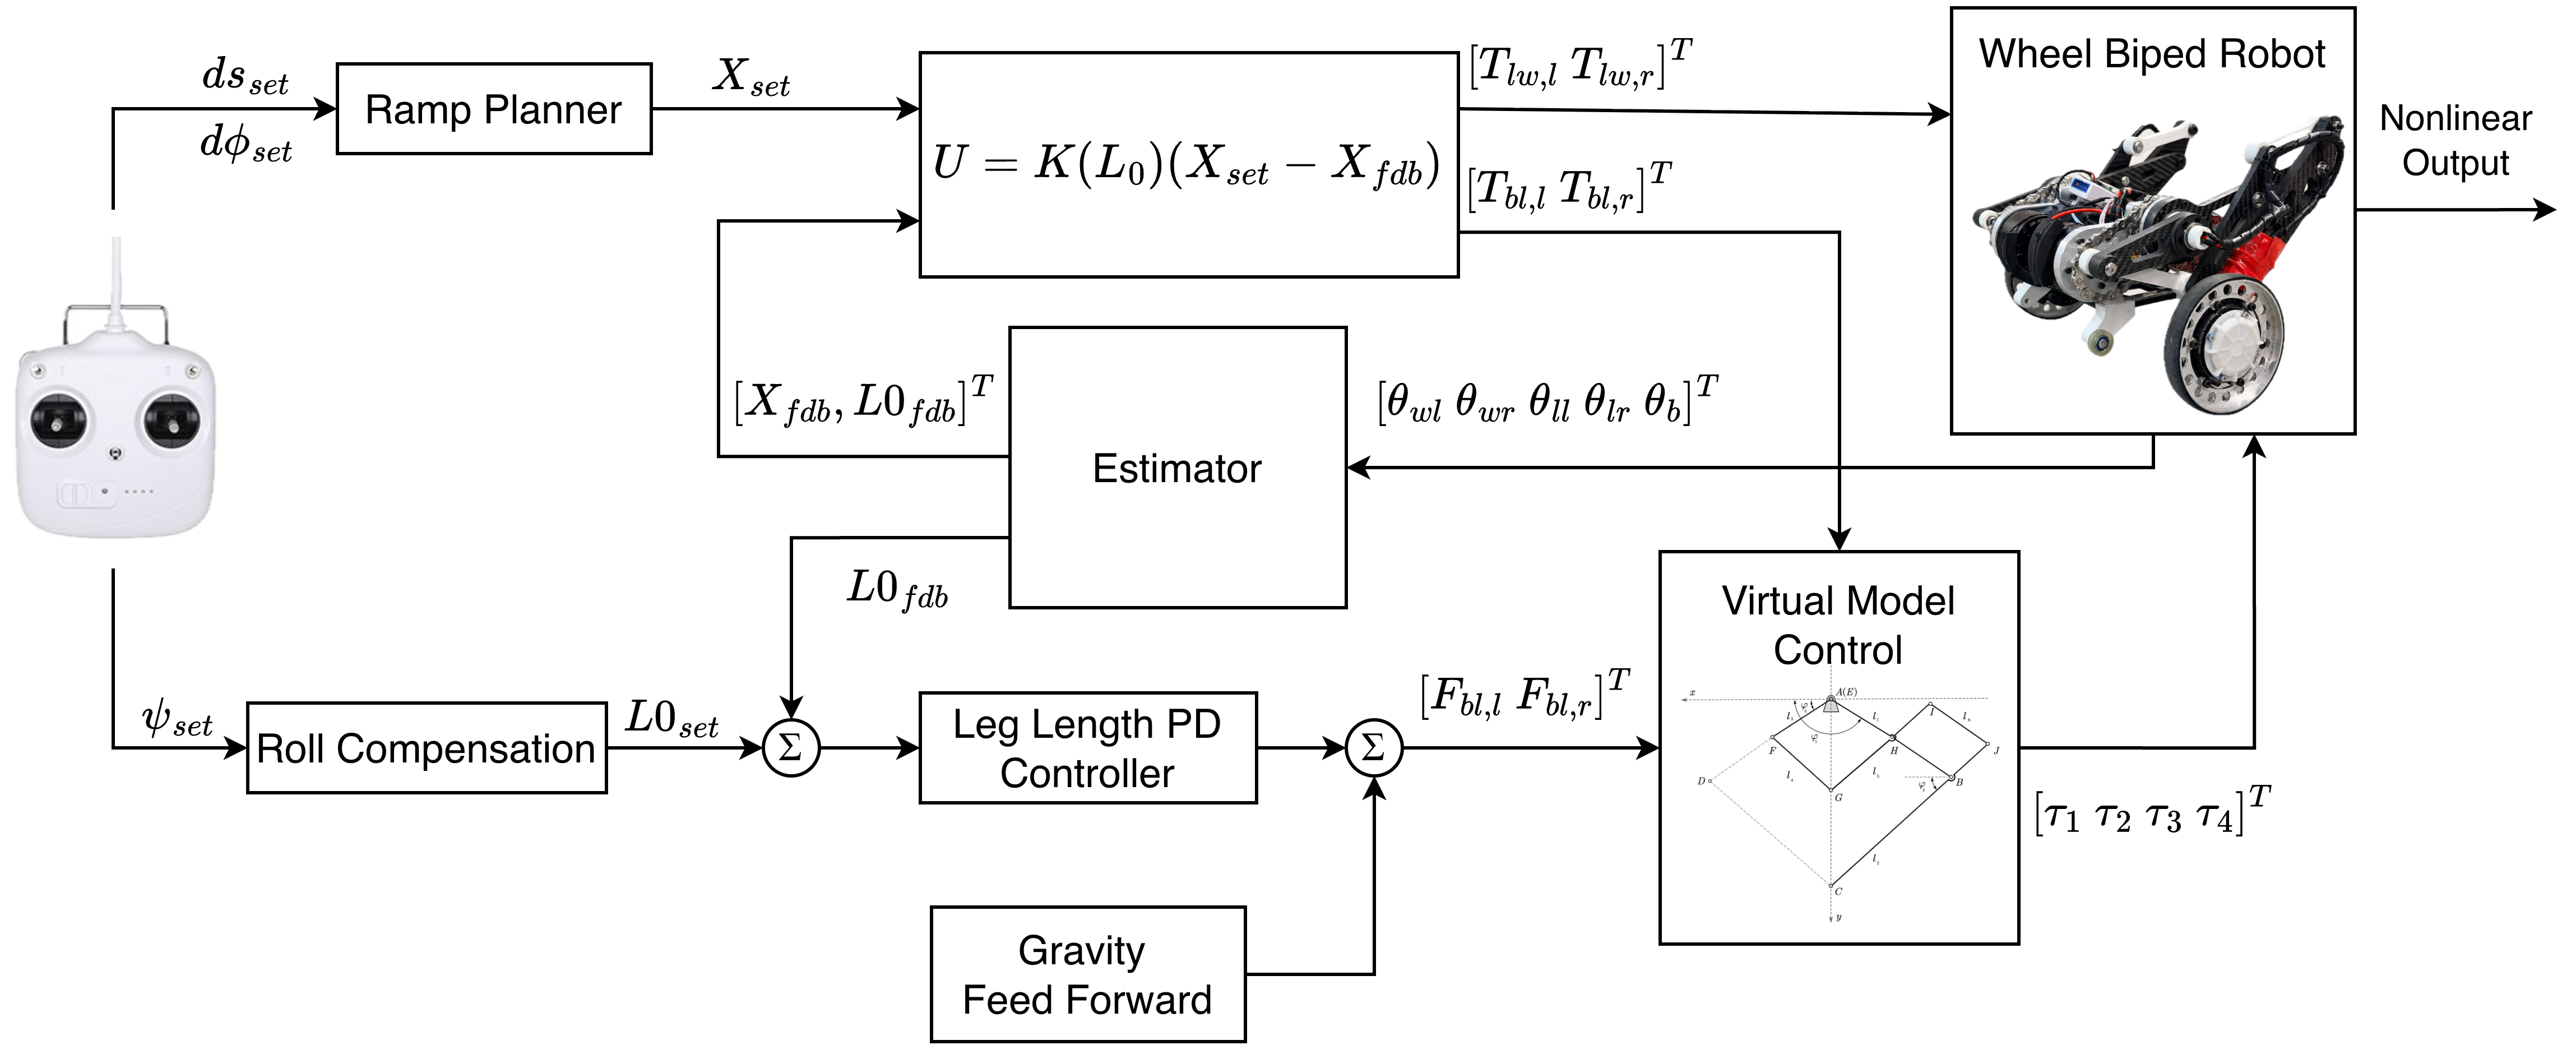
\includegraphics[width=1.0\textwidth]{figures/ch04/control_structure.png}
  \caption{整体控制框图}
  \label{fig:control-structure}
\end{figure}

上述架构的核心思想在于“全局平衡与局部支撑解耦”。其中，LQR 负责处理整机平衡、运动趋势和腿摆控制量，VMC 负责处理腿长方向的局部支撑行为，滚转补偿负责补足运动模型未展开的侧向稳定问题。这样既保持了控制结构清晰，又能体现本文“轻量级、可实时部署”的方法定位。

\section{LQR 控制器设计}

\subsection{控制目标与状态变量选取}

在分层控制框架中，运动控制器负责机器人在前进方向上的站立平衡、速度跟踪以及扰动恢复。考虑到机器人在直立工况附近可近似为多输入多输出线性系统，本文将第三章建立的五自由度动力学模型在线性化后用于 LQR 设计。为保持与原始模型的一致性，仍选取左右轮转角、左右腿摆角和机体俯仰角作为独立广义坐标，即
\begin{equation}
  \boldsymbol{q} =
  \begin{bmatrix}
    \theta_{wl} & \theta_{wr} & \theta_{ll} & \theta_{lr} & \theta_b
  \end{bmatrix}^{\mathsf{T}}
  \label{eq:full-generalized-coordinate}
\end{equation}
输入向量定义为
\begin{equation}
  \boldsymbol{u} =
  \begin{bmatrix}
    T_{lw,l} & T_{lw,r} & T_{bl,l} & T_{bl,r}
  \end{bmatrix}^{\mathsf{T}}
  \label{eq:full-input-vector}
\end{equation}

为了使状态量更贴近机器人实际运动状态，本文将前进位移 $s$、偏航角 $\phi$、左右腿摆角和机体俯仰角作为控制器设计中的物理状态，并构造完整状态向量
\begin{equation}
  \boldsymbol{x}
  =
  \begin{bmatrix}
    s & \dot{s} & \phi & \dot{\phi} & \theta_{ll} & \dot{\theta}_{ll} &
    \theta_{lr} & \dot{\theta}_{lr} & \theta_b & \dot{\theta}_b
  \end{bmatrix}^{\mathsf{T}}.
  \label{eq:full-state-vector}
\end{equation}
其中，$s$ 与 $\phi$ 由第三章给出的轮系运动学关系计算得到。相较于直接使用广义坐标，\eqref{eq:full-state-vector} 中的状态量具有更清晰的物理意义，更便于从“平衡、转向、腿摆、俯仰”四类目标出发进行权重设计和实验分析。

\subsection{线性状态空间模型构建}

选取机器人静态直立工况作为平衡工作点，对第三章推导得到的非线性动力学方程进行小角度线性化，可得广义动力学形式
\begin{equation}
  \boldsymbol{M}\ddot{\boldsymbol{q}} + \boldsymbol{K}\boldsymbol{q} = \boldsymbol{E}\boldsymbol{u},
  \label{eq:linearized-generalized-dynamics}
\end{equation}
其中，$\boldsymbol{M}$ 为平衡点处的等效惯性矩阵，$\boldsymbol{K}$ 为线性化后的重力与耦合项矩阵，$\boldsymbol{E}$ 为输入分配矩阵。由 $\boldsymbol{M}$ 的非奇异性，可将上式改写为显式加速度形式
\begin{equation}
  \ddot{\boldsymbol{q}}
  =
  \boldsymbol{A}_{\mathrm{dyn}} \boldsymbol{q}
  +
  \boldsymbol{B}_{\mathrm{dyn}} \boldsymbol{u}
  \qquad
  \boldsymbol{A}_{\mathrm{dyn}} = -\boldsymbol{M}^{-1}\boldsymbol{K}
  \qquad
  \boldsymbol{B}_{\mathrm{dyn}} = \boldsymbol{M}^{-1}\boldsymbol{E}
  \label{eq:qdd-dyn}
\end{equation}

第三章已经给出轮系与腿部运动学映射关系，因此前进位移和偏航角满足
\begin{equation}
  s = \frac{R_w}{2}\left(\theta_{wl} + \theta_{wr}\right)
  \label{eq:s-kinematic-map}
\end{equation}
\begin{equation}
  \phi
  =
  \frac{R_w}{2R_l}\left(-\theta_{wl} + \theta_{wr}\right)
  -
  \frac{l_l}{2R_l}\sin \theta_{ll}
  +
  \frac{l_r}{2R_l}\sin \theta_{lr}
  \label{eq:phi-kinematic-map}
\end{equation}
在平衡点附近将\eqref{eq:s-kinematic-map} 和\eqref{eq:phi-kinematic-map} 线性化，并将广义坐标表达式转换为\eqref{eq:full-state-vector} 所示的物理状态后，主控制器使用的标准状态空间方程可写为
\begin{equation}
  \dot{\boldsymbol{x}} = \boldsymbol{A}\boldsymbol{x} + \boldsymbol{B}\boldsymbol{u}
  \label{eq:linear-state-space}
\end{equation}

\eqref{eq:linear-state-space} 给出了用于运动控制器设计的线性模型。与原始非线性模型相比，该表达式在保留轮系、腿部和俯仰耦合关系的同时，显著降低了在线求解难度。

\subsection{LQR 反馈律设计}

对于\eqref{eq:linear-state-space} 描述的十维四输入线性时不变系统，本文采用线性二次型调节器（LQR）作为运动控制器\cite{klemm2020lqr}。
选择 LQR 的原因在于：一方面，机器人在站立与匀速行进工况下的大部分控制任务均围绕直立平衡点展开，线性模型能够较好描述该工作区间内的主要动力学特性；另一方面，LQR 仅需离线求解 Riccati 方程，在线阶段只进行矩阵乘法运算，计算量小，便于嵌入式实时实现。

定义无穷时域二次性能指标为
\begin{equation}
  J =
  \int_{0}^{\infty}
  \left(
    \delta \boldsymbol{x}^{\mathsf{T}}\boldsymbol{Q}\,\delta \boldsymbol{x}
    +
    \delta \boldsymbol{u}^{\mathsf{T}}\boldsymbol{R}\,\delta \boldsymbol{u}
  \right)\dd t,
  \label{eq:lqr-cost}
\end{equation}
其中，$\boldsymbol{Q} \succeq 0$ 为状态加权矩阵，$\boldsymbol{R} \succ 0$ 为控制加权矩阵。$\boldsymbol{Q}$ 用于度量前进位移、偏航角、腿摆角和机体俯仰角等状态的偏差程度；$\boldsymbol{R}$ 用于约束轮电机与腿部驱动器的输出幅值，避免过大的控制输入导致执行器饱和和结构冲击。在实际设计中，可适当增大 $\theta_b$、$\dot{\theta}_b$ 和 $\dot{s}$ 的权重，以提高姿态稳定与速度恢复能力。

对于增量系统
\begin{equation}
  \delta \dot{\boldsymbol{x}}
  =
  \boldsymbol{A}\delta \boldsymbol{x}
  +
  \boldsymbol{B}\delta \boldsymbol{u},
  \label{eq:lqr-system}
\end{equation}
若存在正定矩阵 $\boldsymbol{P}$ 满足连续时间代数 Riccati 方程
\begin{equation}
  \boldsymbol{A}^{\mathsf{T}}\boldsymbol{P}
  +
  \boldsymbol{P}\boldsymbol{A}
  -
  \boldsymbol{P}\boldsymbol{B}\boldsymbol{R}^{-1}\boldsymbol{B}^{\mathsf{T}}\boldsymbol{P}
  +
  \boldsymbol{Q}
  =
  \boldsymbol{0},
  \label{eq:riccati}
\end{equation}
则最优状态反馈律为
\begin{equation}
  \delta \boldsymbol{u}
  =
  -\boldsymbol{K}\delta \boldsymbol{x},
  \qquad
  \boldsymbol{K} =
  \boldsymbol{R}^{-1}\boldsymbol{B}^{\mathsf{T}}\boldsymbol{P}.
  \label{eq:lqr-law}
\end{equation}
因此主控制器输出可写为
\begin{equation}
  \boldsymbol{u}
  =
  \begin{bmatrix}
    T_{lw,l} & T_{lw,r} & T_{bl,l} & T_{bl,r}
  \end{bmatrix}^{\mathsf{T}}
  =
  -
  \boldsymbol{K}
  \left(
    \boldsymbol{x} - \boldsymbol{x}_d
  \right),
  \label{eq:lqr-output}
\end{equation}
其中，$\boldsymbol{x}_d$ 为期望状态向量。静态站立任务中通常取 $\boldsymbol{x}_d = \boldsymbol{0}$；速度跟踪或转向任务中，则可通过设置 $\dot{s}_d$、$\phi_d$ 等参考量生成相应的平衡工作点。

\section{VMC 控制器设计}

\subsection{腿长控制律}

LQR 主控制器能够有效处理前进方向上的全局平衡，但它并不直接负责腿长调节、缓冲支撑和越障时的局部运动组织。
考虑到闭环五连杆机构在关节空间中耦合较强，而虚拟腿长度和虚拟腿摆角具有更明确的物理含义，本文在腿部控制中仍采用任务空间描述：腿长方向由 VMC 构造轴向支撑力，腿摆方向直接沿用 LQR 输出的控制量。

对于左、右腿，分别定义任务空间状态为
\begin{equation}
  \boldsymbol{x}_{v,i} =
  \begin{bmatrix}
    l_i & \theta_{l,i}
  \end{bmatrix}^{\mathsf{T}},
  \qquad i \in \{l,r\},
  \label{eq:leg-task-state}
\end{equation}
其中，$l_i$ 表示第 $i$ 条腿的虚拟腿长，$\theta_{l,i}$ 表示其虚拟腿摆角。针对腿长方向，构造虚拟弹簧阻尼器，并引入重力前馈补偿，其轴向虚拟力为
\begin{equation}
  F_{l,i}^{\ast}
  =
  K_l (l_{d,i} - l_i)
  +
  D_l (\dot{l}_{d,i} - \dot{l}_i)
  +
  \frac{1}{2} mg \cos\theta_{l,i},
  \qquad i \in \{l,r\}.
  \label{eq:leg-force-law}
\end{equation}
其中，$m$ 为机器人的部分或整体等效质量，$\frac{1}{2} m g \cos\theta_{l,i}$ 为在此摆角下单腿分担的重力前馈项。\eqref{eq:leg-force-law} 使腿部在支撑阶段表现为具有等效刚度和阻尼的虚拟支撑单元，从而实现机体高度维持、落地缓冲和腿长振荡抑制。与直接进行关节位置控制相比，这种写法更符合机器人与地面发生力学作用时的控制需求，也更便于在不同工况下通过少量参数完成行为切换。

在腿摆方向，本文不再额外构造 PD 修正项，而是直接采用 LQR 主控制器输出的对应腿部控制量。记任务空间中的腿摆虚拟转矩为 $T_{\theta,i}^{\ast}$，则有
\begin{equation}
  T_{\theta,i}^{\ast} = T_{bl,i}^{\ast},
  \qquad i \in \{l,r\}.
  \label{eq:leg-swing-lqr-input}
\end{equation}
其中，$T_{bl,i}^{\ast}$ 来自\eqref{eq:lqr-output}。这样处理可以避免在腿摆方向重复引入局部闭环，使腿摆控制量与线性化平衡模型中的输入保持一致。

因此，左右腿的任务空间控制量可写为
\begin{equation}
  \boldsymbol{F}_{v,i}^{\ast}
  =
  \begin{bmatrix}
    F_{l,i}^{\ast} \\
    T_{\theta,i}^{\ast}
  \end{bmatrix},
  \qquad i \in \{l,r\}.
  \label{eq:task-space-input}
\end{equation}

\subsection{任务空间到关节空间的力矩映射}

由第三章给出的虚拟腿雅可比矩阵 $\boldsymbol{J}_{v,i}$ 和虚功原理，任务空间控制量到实际关节空间的映射可写为
\begin{equation}
  \boldsymbol{\tau}_{i}^{\ast}
  =
  \boldsymbol{J}_{v,i}^{\mathsf{T}}\boldsymbol{F}_{v,i}^{\ast},
  \qquad i \in \{l,r\}.
  \label{eq:leg-joint-torque}
\end{equation}
其中，$\boldsymbol{\tau}_{i}^{\ast}$ 为第 $i$ 条腿对应主动关节的驱动力矩向量。\eqref{eq:leg-joint-torque} 将“任务空间中的腿长支撑力与 LQR 腿摆控制量”转换为“关节空间中的可执行力矩命令”，使闭环五连杆机构仍可在虚拟腿描述下进行直观控制。因此，本文并不在第四章重复推导闭环机构运动学细节，而是直接调用第三章建立的映射关系，以减少章节间重复。

\section{机体滚转角补偿}

第三章建立的主动力学模型主要刻画前进方向、腿摆和机体俯仰之间的耦合运动。根据第三章基本假设，整机主动力学分析中暂不展开滚转角、左右支撑力差异和侧向惯性力矩的影响。对于实际样机而言，这一模型已经能够覆盖站立和平地直行时的主要动力学特征，但在上下坡、单边桥、横向扰动和转向等工况下，机器人仍会出现明显的侧向滚转。特别是在转向速度较高时，向心力会改变左右侧的实际支撑状态。如果仍按水平地面条件分配推力并调节腿长，机体容易向外侧倾斜，左右腿支撑也会逐渐失衡，进而影响转向过程中的姿态稳定性。

基于上述考虑，本文在原有控制结构之外增加滚转角补偿环节，并采用一种基于几何关系的腿长差修正方法。其基本思路是：根据测得的滚转角以及当前左右腿的几何状态，计算出应施加的期望腿长差，再将这一修正量叠加到腿长通道参考值中，以抑制机体侧倾趋势。该方法不需要改动运动控制器和 VMC 的主体结构，实现上也较为直接，适合在嵌入式平台上实时运行。

在单边桥或侧向不平整地面工况下，机体滚转角可以理解为机器人相对于局部支撑平面的姿态偏差。设左右腿当前腿长分别为 $l_l$ 和 $l_r$，半轮距为 $b$，滚转角为 $\gamma$。由几何关系定义等效坡角 $\delta_{\mathrm{roll}}$，其正切形式为
\begin{equation}
  \tan \delta_{\mathrm{roll}}
  =
  \frac{
    (l_r-l_l)\cos\gamma + 2b\sin\gamma
  }{
    (l_l-l_r)\sin\gamma + 2b\cos\gamma
  }.
  \label{eq:roll-delta}
\end{equation}

进一步地，由右腿一侧的几何关系，机体中心相对于局部支撑平面的等效高度为
\begin{equation}
  h
  =
  l_r\cos\gamma + b\sin\gamma.
  \label{eq:roll-body-height}
\end{equation}
若希望机体在该等效坡面上保持水平，则左右腿的期望腿长可写为
\begin{equation}
  l_{d,l}^{\mathrm{roll}} = h,
  \qquad
  l_{d,r}^{\mathrm{roll}} = h - 2b\tan \delta_{\mathrm{roll}}.
  \label{eq:roll-leg-target}
\end{equation}
因此，由滚转角引起的期望腿长差为
\begin{equation}
  \Delta l_{\mathrm{roll}}
  =
  l_{d,l}^{\mathrm{roll}} - l_{d,r}^{\mathrm{roll}}
  =
  2b\tan \delta_{\mathrm{roll}}.
  \label{eq:roll-leg-diff}
\end{equation}

\eqref{eq:roll-leg-diff} 给出了该补偿方法的核心结果，即先由当前滚转角和左右腿几何关系求出等效坡角，再将其转化为左右腿的期望腿长差。考虑到腿长通道中已经存在基准腿长控制，为避免直接替换参考量引起指令突变，本文将腿长差的一半以相反符号叠加到左右腿基准腿长上，即
\begin{equation}
  l_{d,l} = l_d + \frac{1}{2}\Delta l_{\mathrm{roll}},
  \qquad
  l_{d,r} = l_d - \frac{1}{2}\Delta l_{\mathrm{roll}},
  \label{eq:roll-leg-superimpose}
\end{equation}
其中，$l_d$ 为对称支撑工况下的公共基准腿长。随后将 $l_{d,l}$ 和 $l_{d,r}$ 代入\eqref{eq:leg-force-law} 对应的左右腿腿长控制器，即可得到滚转补偿后的腿长控制量。

与前述 LQR 和 VMC 控制结构相比，这里的补偿不直接通过支撑力差动构造恢复力矩，而是通过调整左右腿的期望长度来改变局部支撑几何关系。这样处理有两个直接好处：一是物理意义清晰，便于解释单边桥和侧向地形下的姿态修正过程；二是计算量较小，只依赖滚转角、左右腿长和半轮距等基础状态量，便于在嵌入式系统中实现。对于转向工况中由推力变化带来的附加侧倾，\eqref{eq:roll-leg-superimpose} 同样可以作为腿长通道的在线修正项，与上层速度控制配合使用，以减小机体外倾趋势。

\section{状态估计器设计}

为支撑上述分层控制策略的在线运行，样机控制系统配置了轮组编码器、腿部关节编码器以及惯性测量单元等基础传感器。轮组编码器用于获取左右轮转角及其变化率；腿部关节编码器结合第三章建立的机构运动学关系，可实时解算左右腿的虚拟腿长 $l_i$、虚拟腿摆角 $\theta_{l,i}$ 及其导数；惯性测量单元用于获取机体俯仰角、滚转角、角速度以及机体加速度。由于轮腿机器人在越过地形突起或发生轻微打滑时，单纯由轮速积分得到的速度容易出现突变，本文在轮速运动学解算的基础上引入惯性加速度观测，并采用卡尔曼滤波（Kalman filter, KF）进行前进速度估计\cite{kalman1960new}。

在状态估计层中，本文需要为 LQR 主控制器提供前进位移 $s$、前进速度 $\dot{s}$、机体俯仰角 $\theta_b$、腿摆角及其变化率等状态，同时为 VMC 腿长控制提供左右腿长及其变化率。机体姿态主要由惯性测量单元获得；腿部任务空间状态由关节编码器和等效五连杆运动学关系解算；前进速度则由轮速解算值与机体惯性加速度融合得到。这样既避免了依赖外部定位系统，也能减小复杂地面接触造成的轮速测量突变。

考虑单侧驱动轮的运动关系。设轮毂电机编码器测得的转子相对定子的角速度为 $\omega_{\mathrm{enc}}$，腿部机构带动轮轴支架相对机体的角速度为 $\dot{\theta}_l$，机体相对惯性系的俯仰角速度为 $\dot{\theta}_b$。在轮端不打滑且近似纯滚动的条件下，驱动轮相对地面的角速度可近似写为
\begin{equation}
  \omega_w
  =
  \omega_{\mathrm{enc}}
  +
  \dot{\theta}_l
  +
  \dot{\theta}_b .
  \label{eq:wheel-ground-angular-velocity}
\end{equation}
由轮半径 $R_w$ 可得到轮轴接地点对应的平动速度
\begin{equation}
  \dot{x}_w = R_w \omega_w .
  \label{eq:wheel-velocity-est}
\end{equation}

对于本文采用的虚拟腿描述，机体质心前向位置与轮轴位置、虚拟腿长度和腿摆角之间存在几何关系。以单侧等效模型说明，若记虚拟腿长度为 $l$，腿摆角为 $\theta_l$，则机体前向速度可写为
\begin{equation}
  \dot{x}_b
  =
  \dot{x}_w
  +
  l \dot{\theta}_l \cos\theta_l
  +
  \dot{l}\sin\theta_l .
  \label{eq:body-velocity-kinematic}
\end{equation}
将\eqref{eq:wheel-velocity-est} 代入上式，即可得到由编码器和姿态角速度解算出的机体前进速度观测量。实际实现中，左右两侧轮组分别计算得到 $\dot{x}_{b,l}$ 和 $\dot{x}_{b,r}$，直线运动时取二者平均作为前进速度观测值
\begin{equation}
  \dot{s}_{\mathrm{enc}}
  =
  \frac{1}{2}
  \left(
    \dot{x}_{b,l}
    +
    \dot{x}_{b,r}
  \right).
  \label{eq:encoder-forward-velocity}
\end{equation}
同时，左右轮速度差可用于估计偏航角速度，并结合第三章轮系运动学关系得到偏航角 $\phi$ 及其变化率。

轮速运动学解算具有计算量小、响应快的优点，但其可靠性依赖纯滚动假设。当机器人经过地形突起、轮端短时离地或发生打滑时，轮速会出现瞬时突变，直接作为控制反馈可能导致轮端力矩反向冲击。为抑制该问题，本文将惯性测量单元得到的前向加速度作为第二类观测量，并构造二状态离散 KF 对前进速度进行递推估计。

定义观测器状态为
\begin{equation}
  \boldsymbol{x}_{o}
  =
  \begin{bmatrix}
    v & a
  \end{bmatrix}^{\mathsf{T}},
  \label{eq:observer-state}
\end{equation}
其中，$v$ 为机体前进速度，$a$ 为机体前向加速度。KF 的预测模型采用匀加速度离散模型，可写为
\begin{equation}
  \boldsymbol{x}_{o,k+1}
  =
  \boldsymbol{F}_k \boldsymbol{x}_{o,k}
  +
  \boldsymbol{\Gamma}_k w_k,
  \qquad
  w_k \sim \mathcal{N}(0,Q_k),
  \label{eq:observer-process}
\end{equation}
其中
\begin{equation}
  \boldsymbol{F}_k
  =
  \begin{bmatrix}
    1 & \Delta t \\
    0 & 1
  \end{bmatrix},
  \qquad
  \boldsymbol{\Gamma}_k
  =
  \begin{bmatrix}
    \frac{1}{2}\Delta t^2 \\
    \Delta t
  \end{bmatrix}.
  \label{eq:observer-matrix}
\end{equation}

KF 的观测向量由轮速运动学解算得到的速度 $\dot{s}_{\mathrm{enc}}$ 和惯性测量单元得到的前向加速度 $a_{\mathrm{imu}}$ 组成，即
\begin{equation}
  \boldsymbol{z}_k
  =
  \begin{bmatrix}
    \dot{s}_{\mathrm{enc}} \\
    a_{\mathrm{imu}}
  \end{bmatrix}
  =
  \boldsymbol{H}_k \boldsymbol{x}_{o,k}
  +
  \boldsymbol{v}_k,
  \qquad
  \boldsymbol{H}_k
  =
  \begin{bmatrix}
    1 & 0 \\
    0 & 1
  \end{bmatrix},
  \label{eq:observer-measurement}
\end{equation}
其中，$\boldsymbol{v}_k \sim \mathcal{N}(\boldsymbol{0},\boldsymbol{R}_k)$ 为测量噪声，测量噪声协方差可取为
\begin{equation}
  \boldsymbol{R}_k
  =
  \begin{bmatrix}
    \sigma_v^2 & 0 \\
    0 & \sigma_a^2
  \end{bmatrix}.
  \label{eq:observer-noise}
\end{equation}
这里，$\sigma_v^2$ 反映轮速解算结果的可信度，$\sigma_a^2$ 反映惯性加速度测量的噪声水平。KF 根据过程噪声协方差 $Q_k$ 和测量噪声协方差 $\boldsymbol{R}_k$ 在预测值与观测值之间分配权重。当地面接触较平稳时，可适当提高轮速观测的权重；当机器人经过凸起或存在打滑风险时，可增大 $\sigma_v^2$，使估计结果更多依赖惯性加速度预测，从而降低速度反馈中的瞬时尖峰。

经过上述估计后，控制器使用的前进速度取观测器输出的 $\hat{v}$，前进位移 $s$ 由 $\hat{v}$ 积分并结合轮系位移进行低频修正。机体俯仰角 $\theta_b$、滚转角 $\gamma$ 及其角速度由惯性测量单元提供，左右虚拟腿长 $l_i$、腿摆角 $\theta_{l,i}$ 及其导数由腿部关节编码器和运动学关系实时解算。最终，状态估计层向上层控制器输出
\begin{equation}
  \hat{\boldsymbol{x}}
  =
  \begin{bmatrix}
    \hat{s} & \hat{\dot{s}} & \hat{\phi} & \hat{\dot{\phi}} &
    \hat{\theta}_{l,l} & \hat{\dot{\theta}}_{l,l} &
    \hat{\theta}_{l,r} & \hat{\dot{\theta}}_{l,r} &
    \hat{\theta}_b & \hat{\dot{\theta}}_b
  \end{bmatrix}^{\mathsf{T}}.
  \label{eq:estimated-controller-state}
\end{equation}
该 KF 估计方式将编码器的快速响应与惯性测量的抗突变能力结合起来，能够为 LQR-VMC 控制器提供更平滑的速度反馈，并降低复杂地面接触对平衡控制的影响。

\section{MuJoCo仿真验证}

为在物理样机制作和进行实验前检查控制器的基本闭环行为并对机构合理性做出验证，
本文在 MuJoCo \cite{todorov2012mujoco}中建立双轮足机器人仿真模型，并将第三章和本章的控制变量与仿真模型中的关节、轮组和机体姿态相对应。
仿真验证的目的不是单独追求模型与样机的完全一致，而是检查设计的 LQR-VMC 分层控制器能否在典型工况下实现稳定闭环，并为后续样机调试提供参数初值和安全边界。

\subsection{仿真模型与控制器实现}

MuJoCo 仿真模型主要包括机体刚体、左右腿部连杆、足端轮组、转动关节、电机执行器以及地面接触参数。
机体质量、轮半径、轮距、腿部连杆尺寸和执行器力矩上限根据第二章样机设计参数设置；
腿部运动学关系则与第三章建立的等效五连杆模型保持一致。
由于本文控制器采用虚拟腿任务空间描述，仿真中不直接将腿部关节作为控制目标，
而是由关节角实时解算左右虚拟腿长 $l_i$、腿摆角 $\theta_{l,i}$ 及其变化率，再将 VMC 腿长输出和 LQR 腿摆输出组成任务空间控制量，并通过雅可比转置映射为关节力矩。

仿真控制器按固定周期1kHz运行。每个控制周期内，程序首先从 MuJoCo 读取机体姿态、轮角、轮速、腿部关节角和关节角速度；
随后完成前进位移、前进速度、虚拟腿长和腿摆角等状态估计；接着执行 LQR 反馈、VMC 腿长支撑计算以及任务空间力矩映射；
最后将轮端力矩和腿部关节力矩下发至 MuJoCo 执行器。该流程与前文控制系统在线工作流程一致，从而能够检验控制律在多刚体接触环境中的实际闭环效果。

\begin{figure}[H]
  \centering
  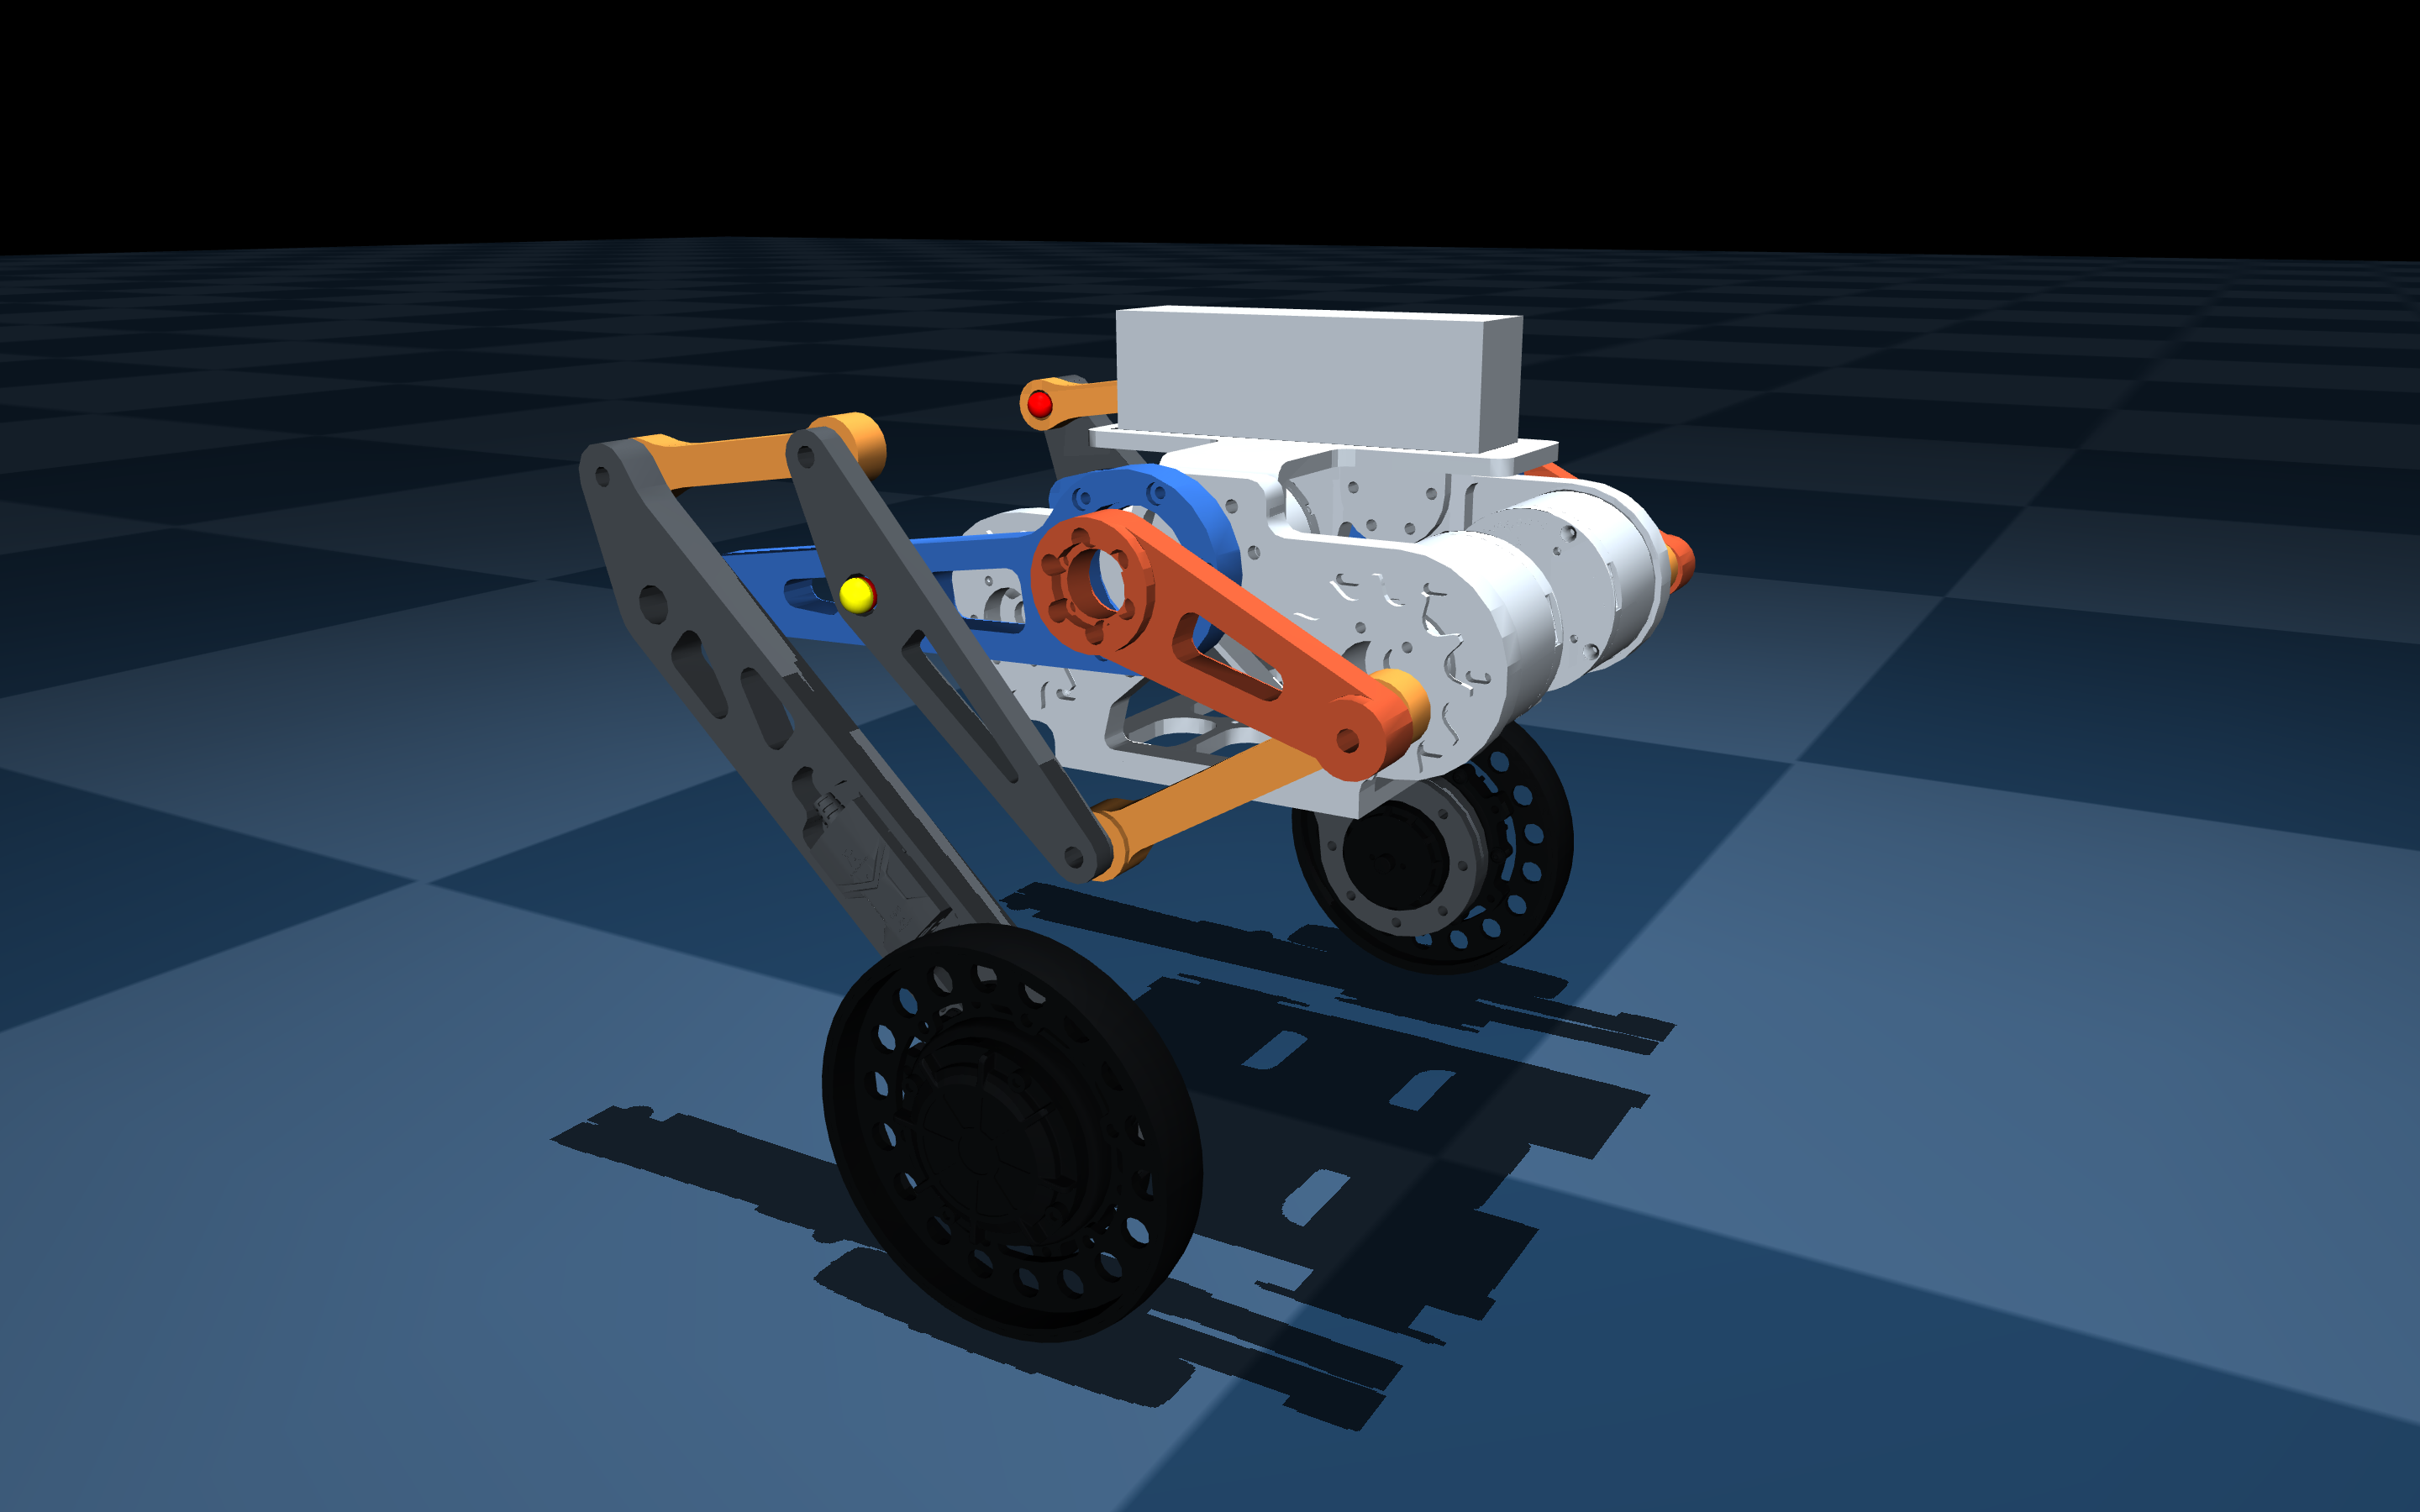
\includegraphics[width=0.95\textwidth]{figures/ch04/mujoco_model.png}
  \caption{MuJoCo 双轮足机器人仿真模型}
  \label{fig:mujoco-model}
\end{figure}

为评价不同控制环节的作用，本文主要记录机体俯仰角 $\theta_b$、前进速度 $\dot{s}$、期望腿长 $l_d$、实际腿长 $l_i$、腿长误差 $l_d-l_i$、轮端力矩 $T_{lw,i}$、腿部关节力矩 $\tau_i$ 。
上述指标分别对应平衡稳定性、速度跟踪能力、腿长调节能力和腿部支撑效果。

\subsection{原地平衡}

原地平衡仿真用于验证 LQR 主控制器与 VMC 腿长控制器能否在直立工作点附近形成稳定闭环。仿真初始时刻给机器人施加一定机体俯仰角偏差，期望前进速度取 $\dot{s}_d=0$，期望偏航角和腿摆角取零，左右腿期望腿长均取基准腿长 $l_d$。控制器启动后，LQR 根据俯仰角、俯仰角速度和轮系状态生成轮端力矩，VMC 则维持左右腿长在期望值附近。

\begin{figure}[H]
  \centering
  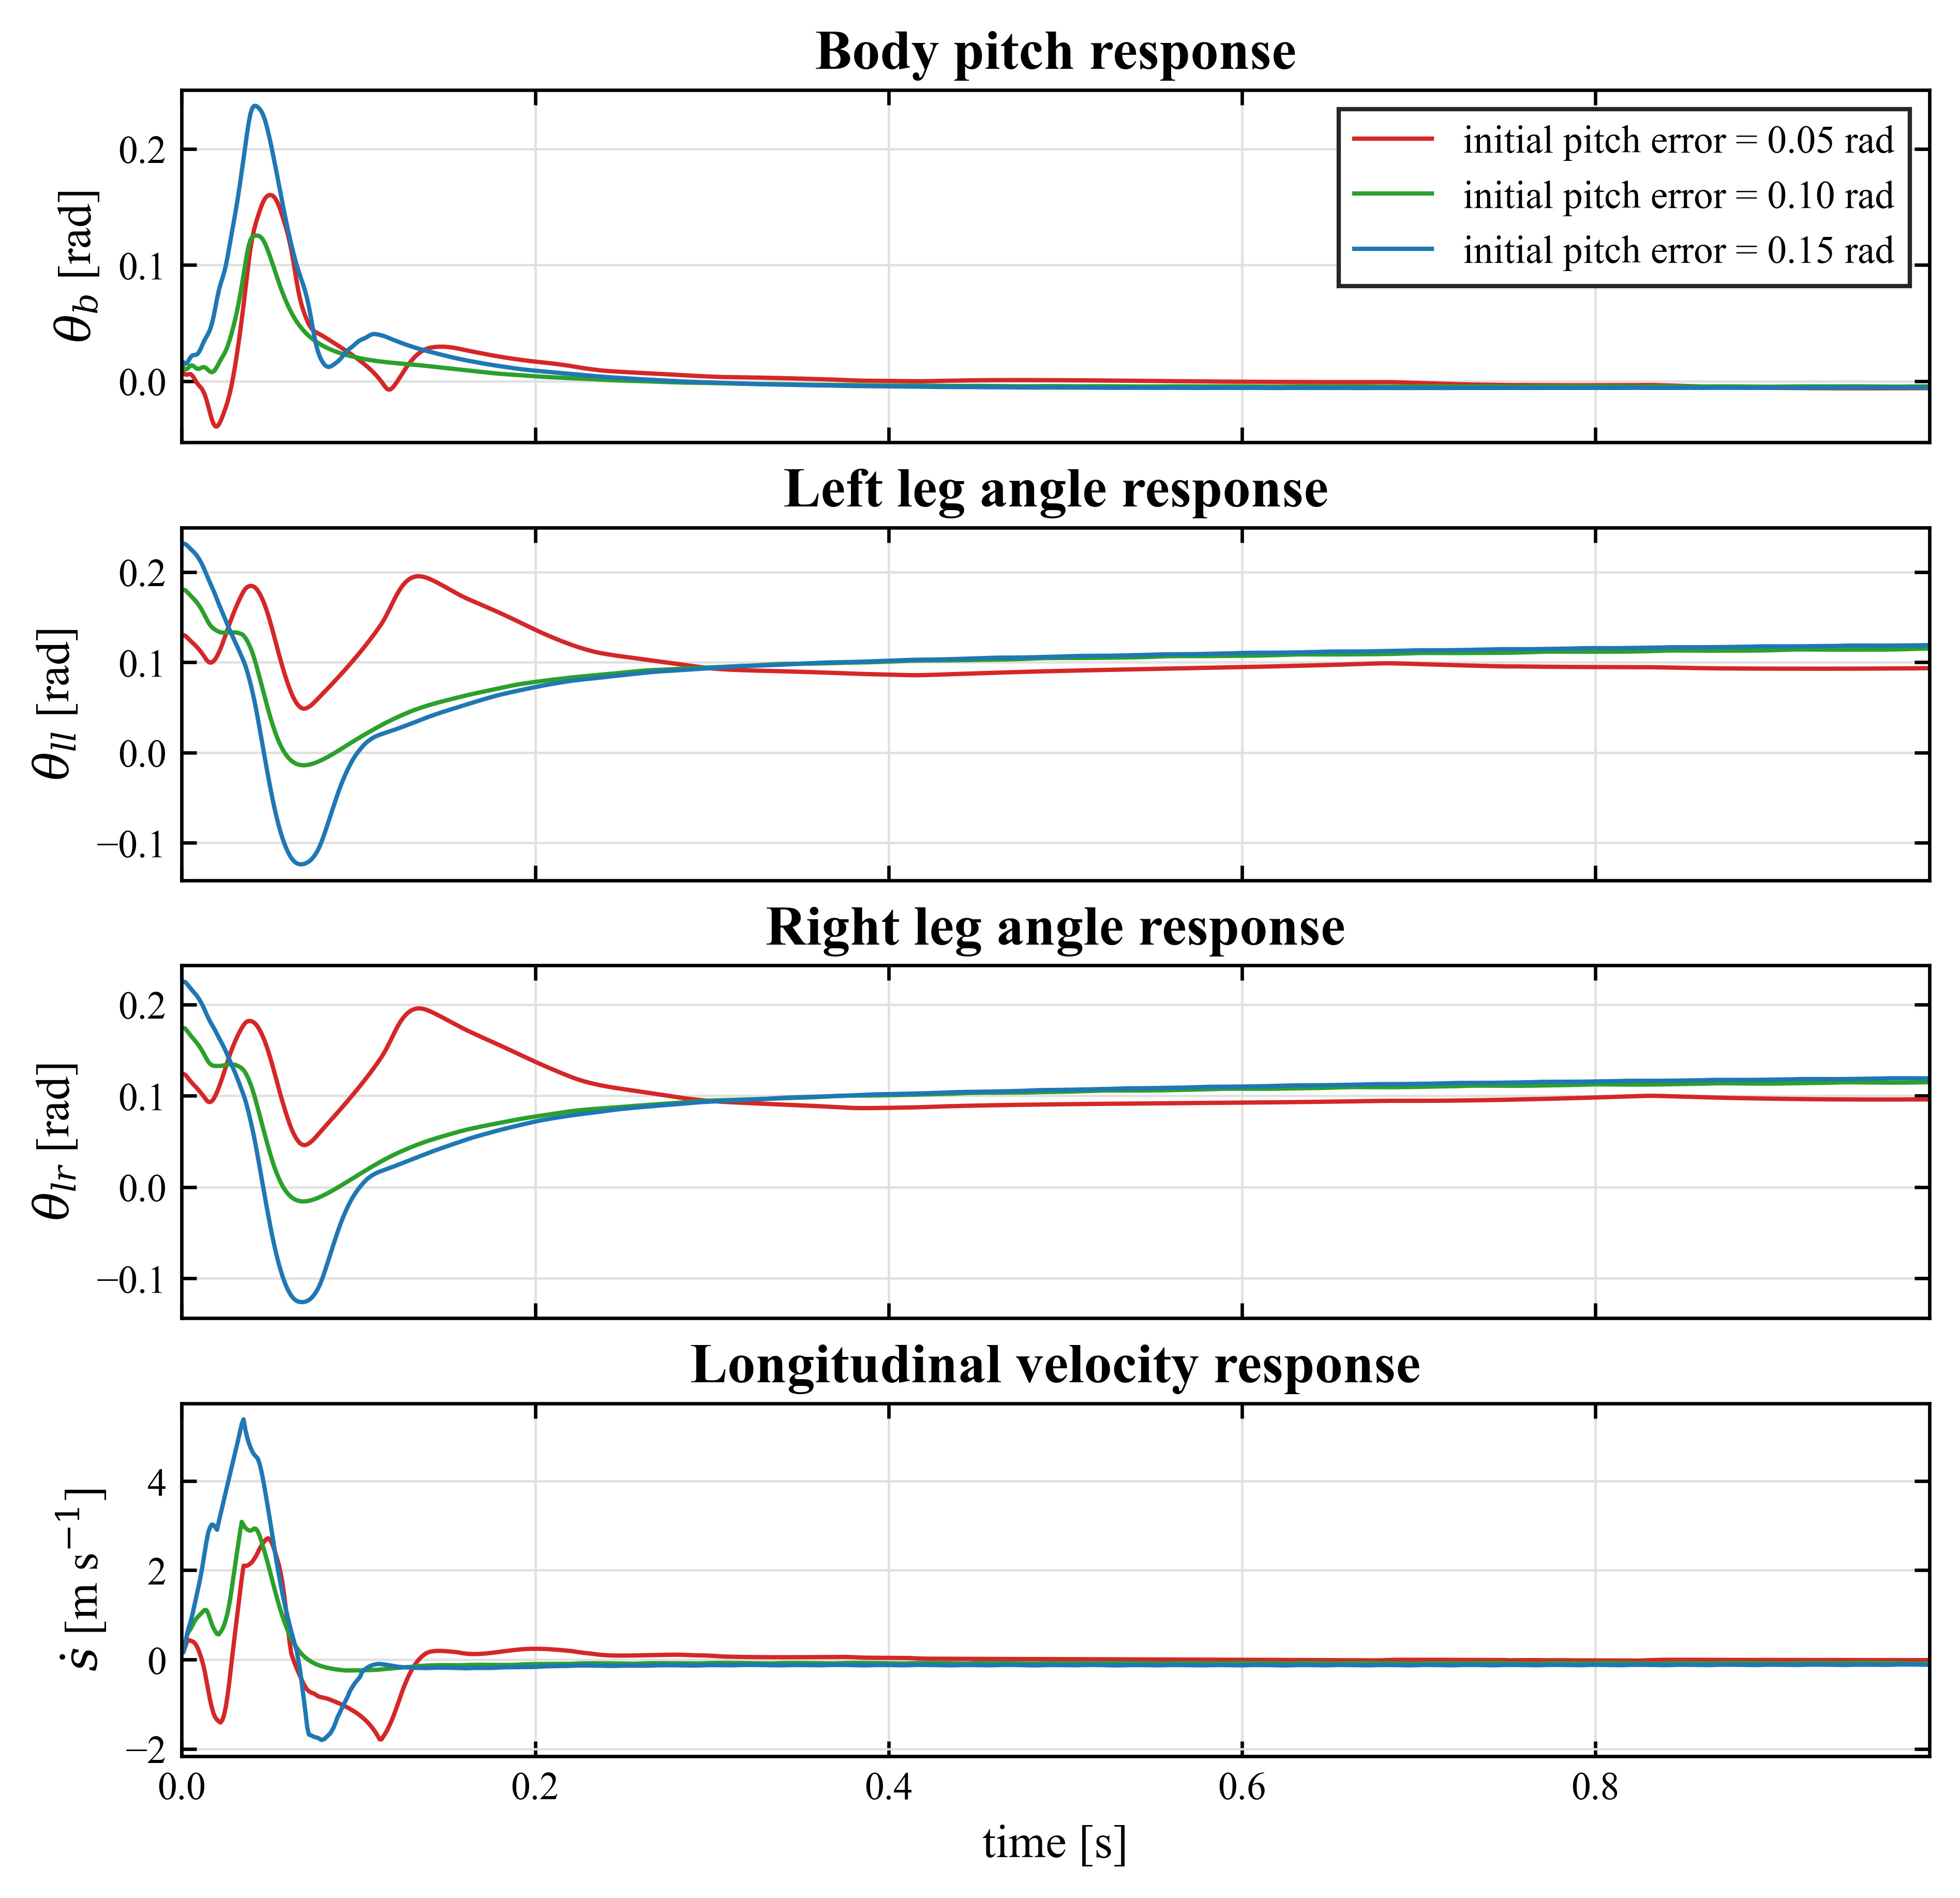
\includegraphics[width=1.0\textwidth]{figures/ch04/balance_response.png}
  \caption{原地平衡工况下的闭环响应。从上至下分别为机体俯仰角、左右腿角、水平速度}
  \label{fig:balance-response}
\end{figure}

仿真结果显示机体俯仰角在0.4s后收敛、左右腿角在0.3s后收敛，水平速度在0.2后收敛。整个控制过程没有明显震荡超调。
说明 LQR 与 VMC 在站立工况下能够协同工作，符合轮式倒立摆通过轮端运动调节机体姿态的物理规律。

\subsection{速度跟踪}

速度跟踪仿真用于检验 LQR 控制器对前进速度和机体姿态的协调能力。仿真中先令机器人保持原地平衡，随后给定水平阶跃速度参考，
由 $0$ 切换至正向速度 $\dot{s}_d$。该工况下，机器人需要通过短时俯仰角偏转产生加速度，并在速度接近期望值后重新回到直立平衡附近。

\begin{figure}[H]
  \centering
  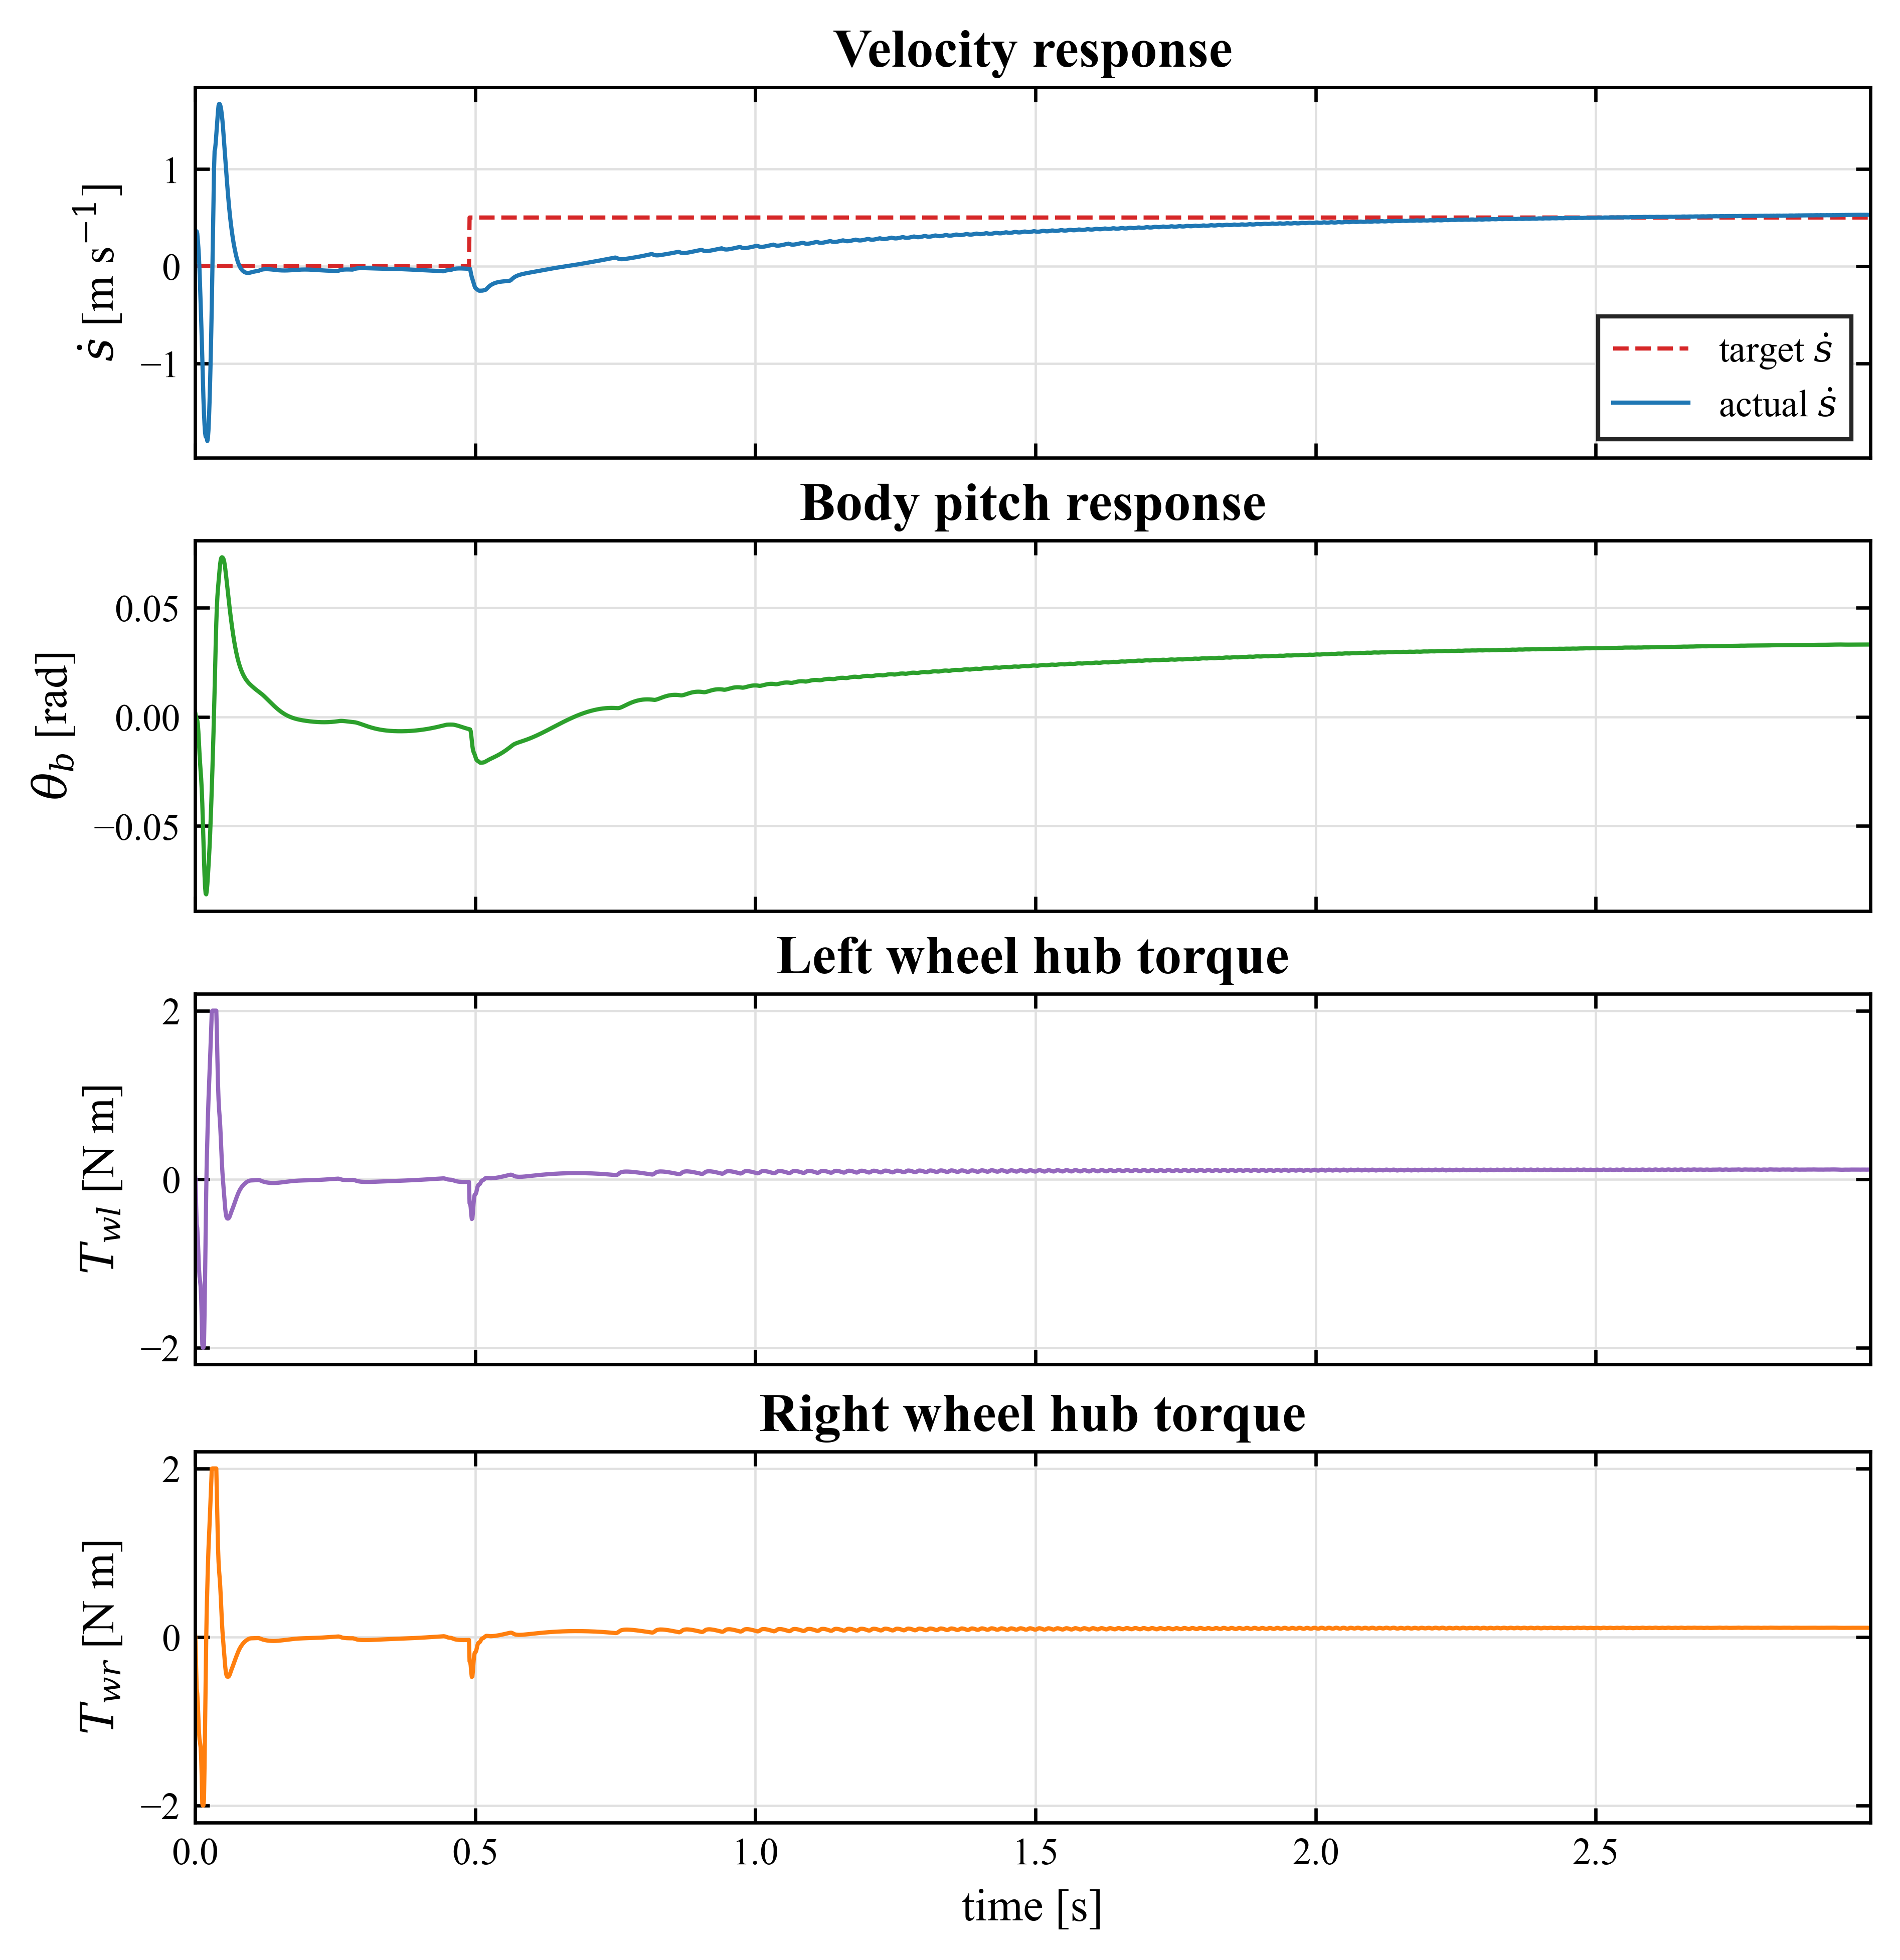
\includegraphics[width=1.0\textwidth]{figures/ch04/velocity_tracking.png}
  \caption{速度跟踪工况下的闭环响应。从上至下分别为前进速度、机体俯仰角、轮端力矩}
  \label{fig:velocity-tracking}
\end{figure}

仿真结果显示实际速度对参考速度的跟随误差在2s后逐渐收敛为0，速度切换时的俯仰角峰值为$0.05rad$， 轮端力矩峰值在$2N\cdot m$内。
说明所设计的 LQR 权重能够在速度跟踪和姿态稳定之间取得可接受的折中。
并且由于轮式倒立摆建模的非最小相位特性，机体想要获得向前的加速度必须先将机身后仰将重心调整至轮轴前方，随后再通过轮端力矩产生加速效果。
由图 \ref{fig:velocity-tracking}可看出$\dot{s}$先为负值后迅速收敛至$0.5m/s$附近，能够反映 LQR 对非最小相位特性的处理能力。

\subsection{扰动恢复}

扰动恢复仿真用于评估控制器对外部冲击的鲁棒性。仿真中保持机器人处于原地平衡状态，分别对机体施加竖直方向和水平方向$2N$的短时脉冲扰动。竖直扰动主要考察 VMC 腿长支撑通道对瞬时载荷变化的缓冲能力，水平扰动主要考察 LQR 平衡控制器对机体俯仰偏差和前后运动趋势的恢复能力。扰动施加位置与方向如\figref{fig:vertical-impulse-scene} 和\figref{fig:horizon-impulse-scene} 所示。

\begin{figure}[H]
  \centering
  \begin{subfigure}[t]{0.38\textwidth}
    \centering
    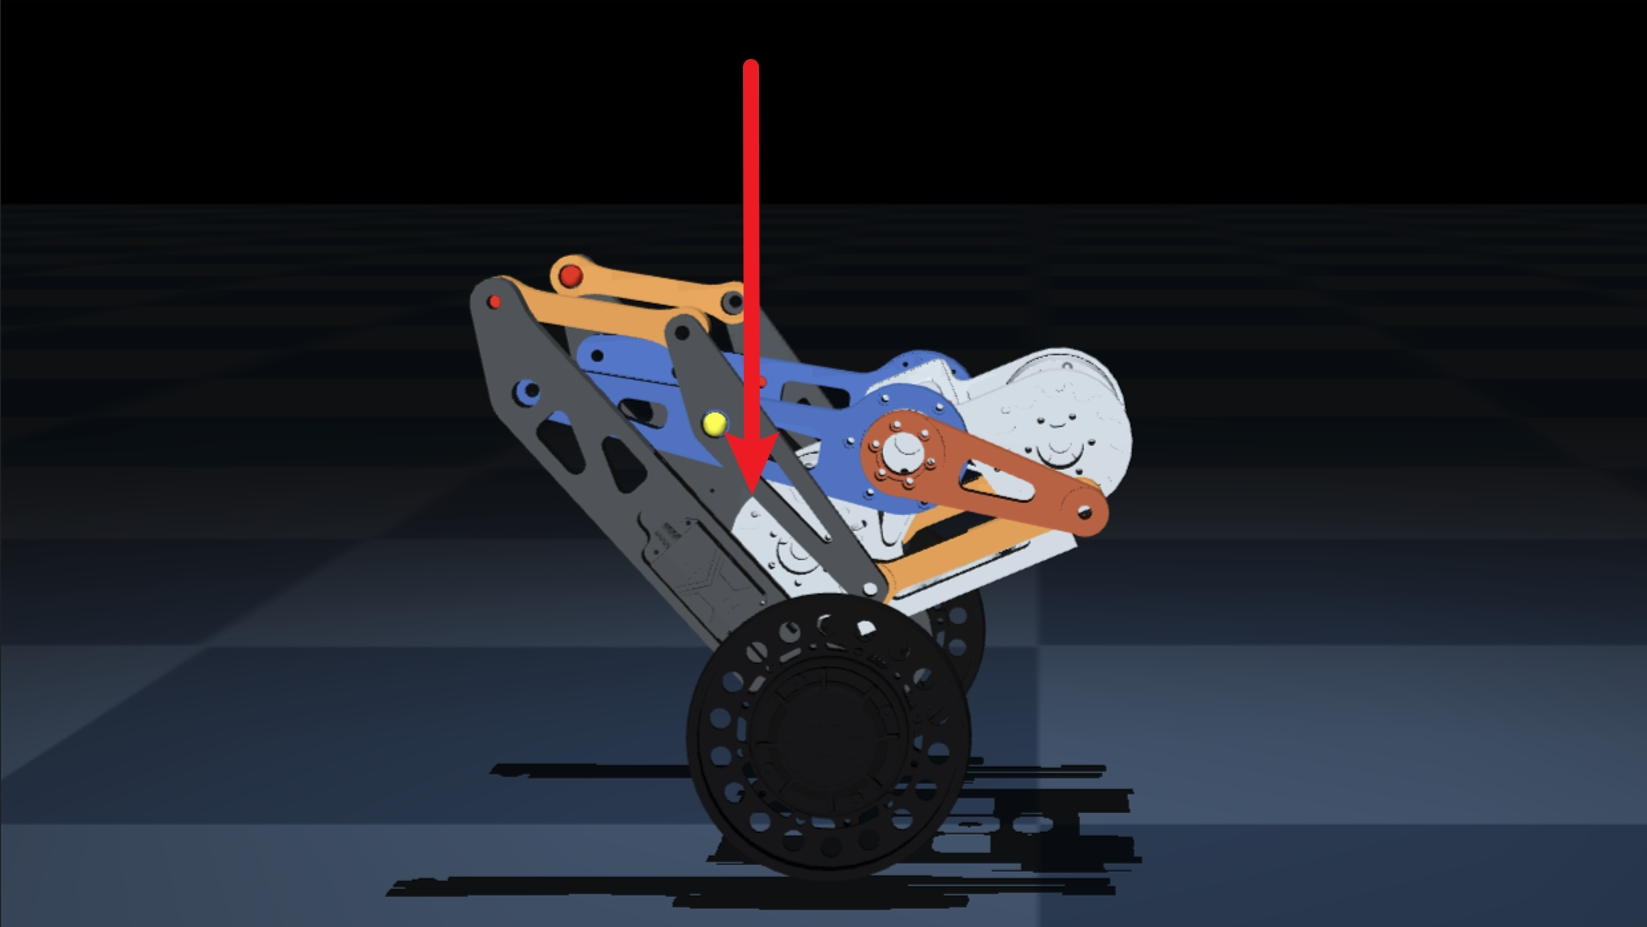
\includegraphics[width=\textwidth]{figures/ch04/vertical_impulse.jpg}
    \caption{竖直脉冲扰动}
    \label{fig:vertical-impulse-scene}
  \end{subfigure}
  \hspace{0.08\textwidth}
  \begin{subfigure}[t]{0.38\textwidth}
    \centering
    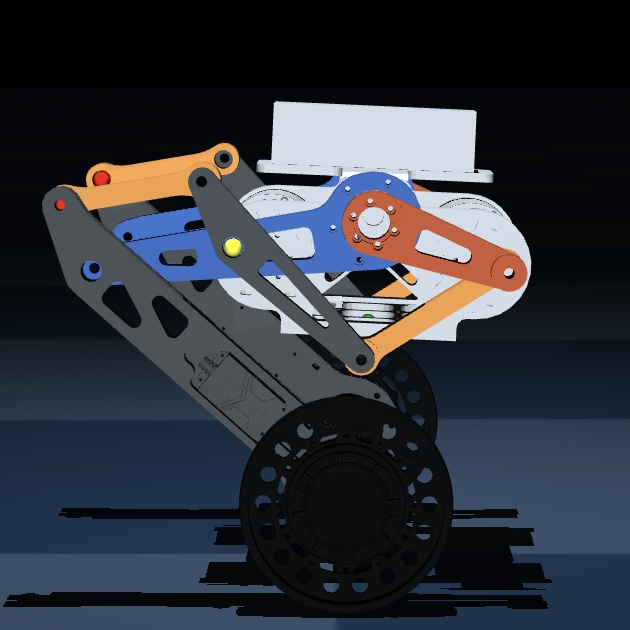
\includegraphics[width=\textwidth]{figures/ch04/horizon_impulse.jpg}
    \caption{水平脉冲扰动}
    \label{fig:horizon-impulse-scene}
  \end{subfigure}
  \caption{不同方向脉冲扰动仿真场景}
  \label{fig:impulse-scene}
\end{figure}

\begin{figure}[H]
  \centering
  \begin{subfigure}[t]{0.49\textwidth}
    \centering
    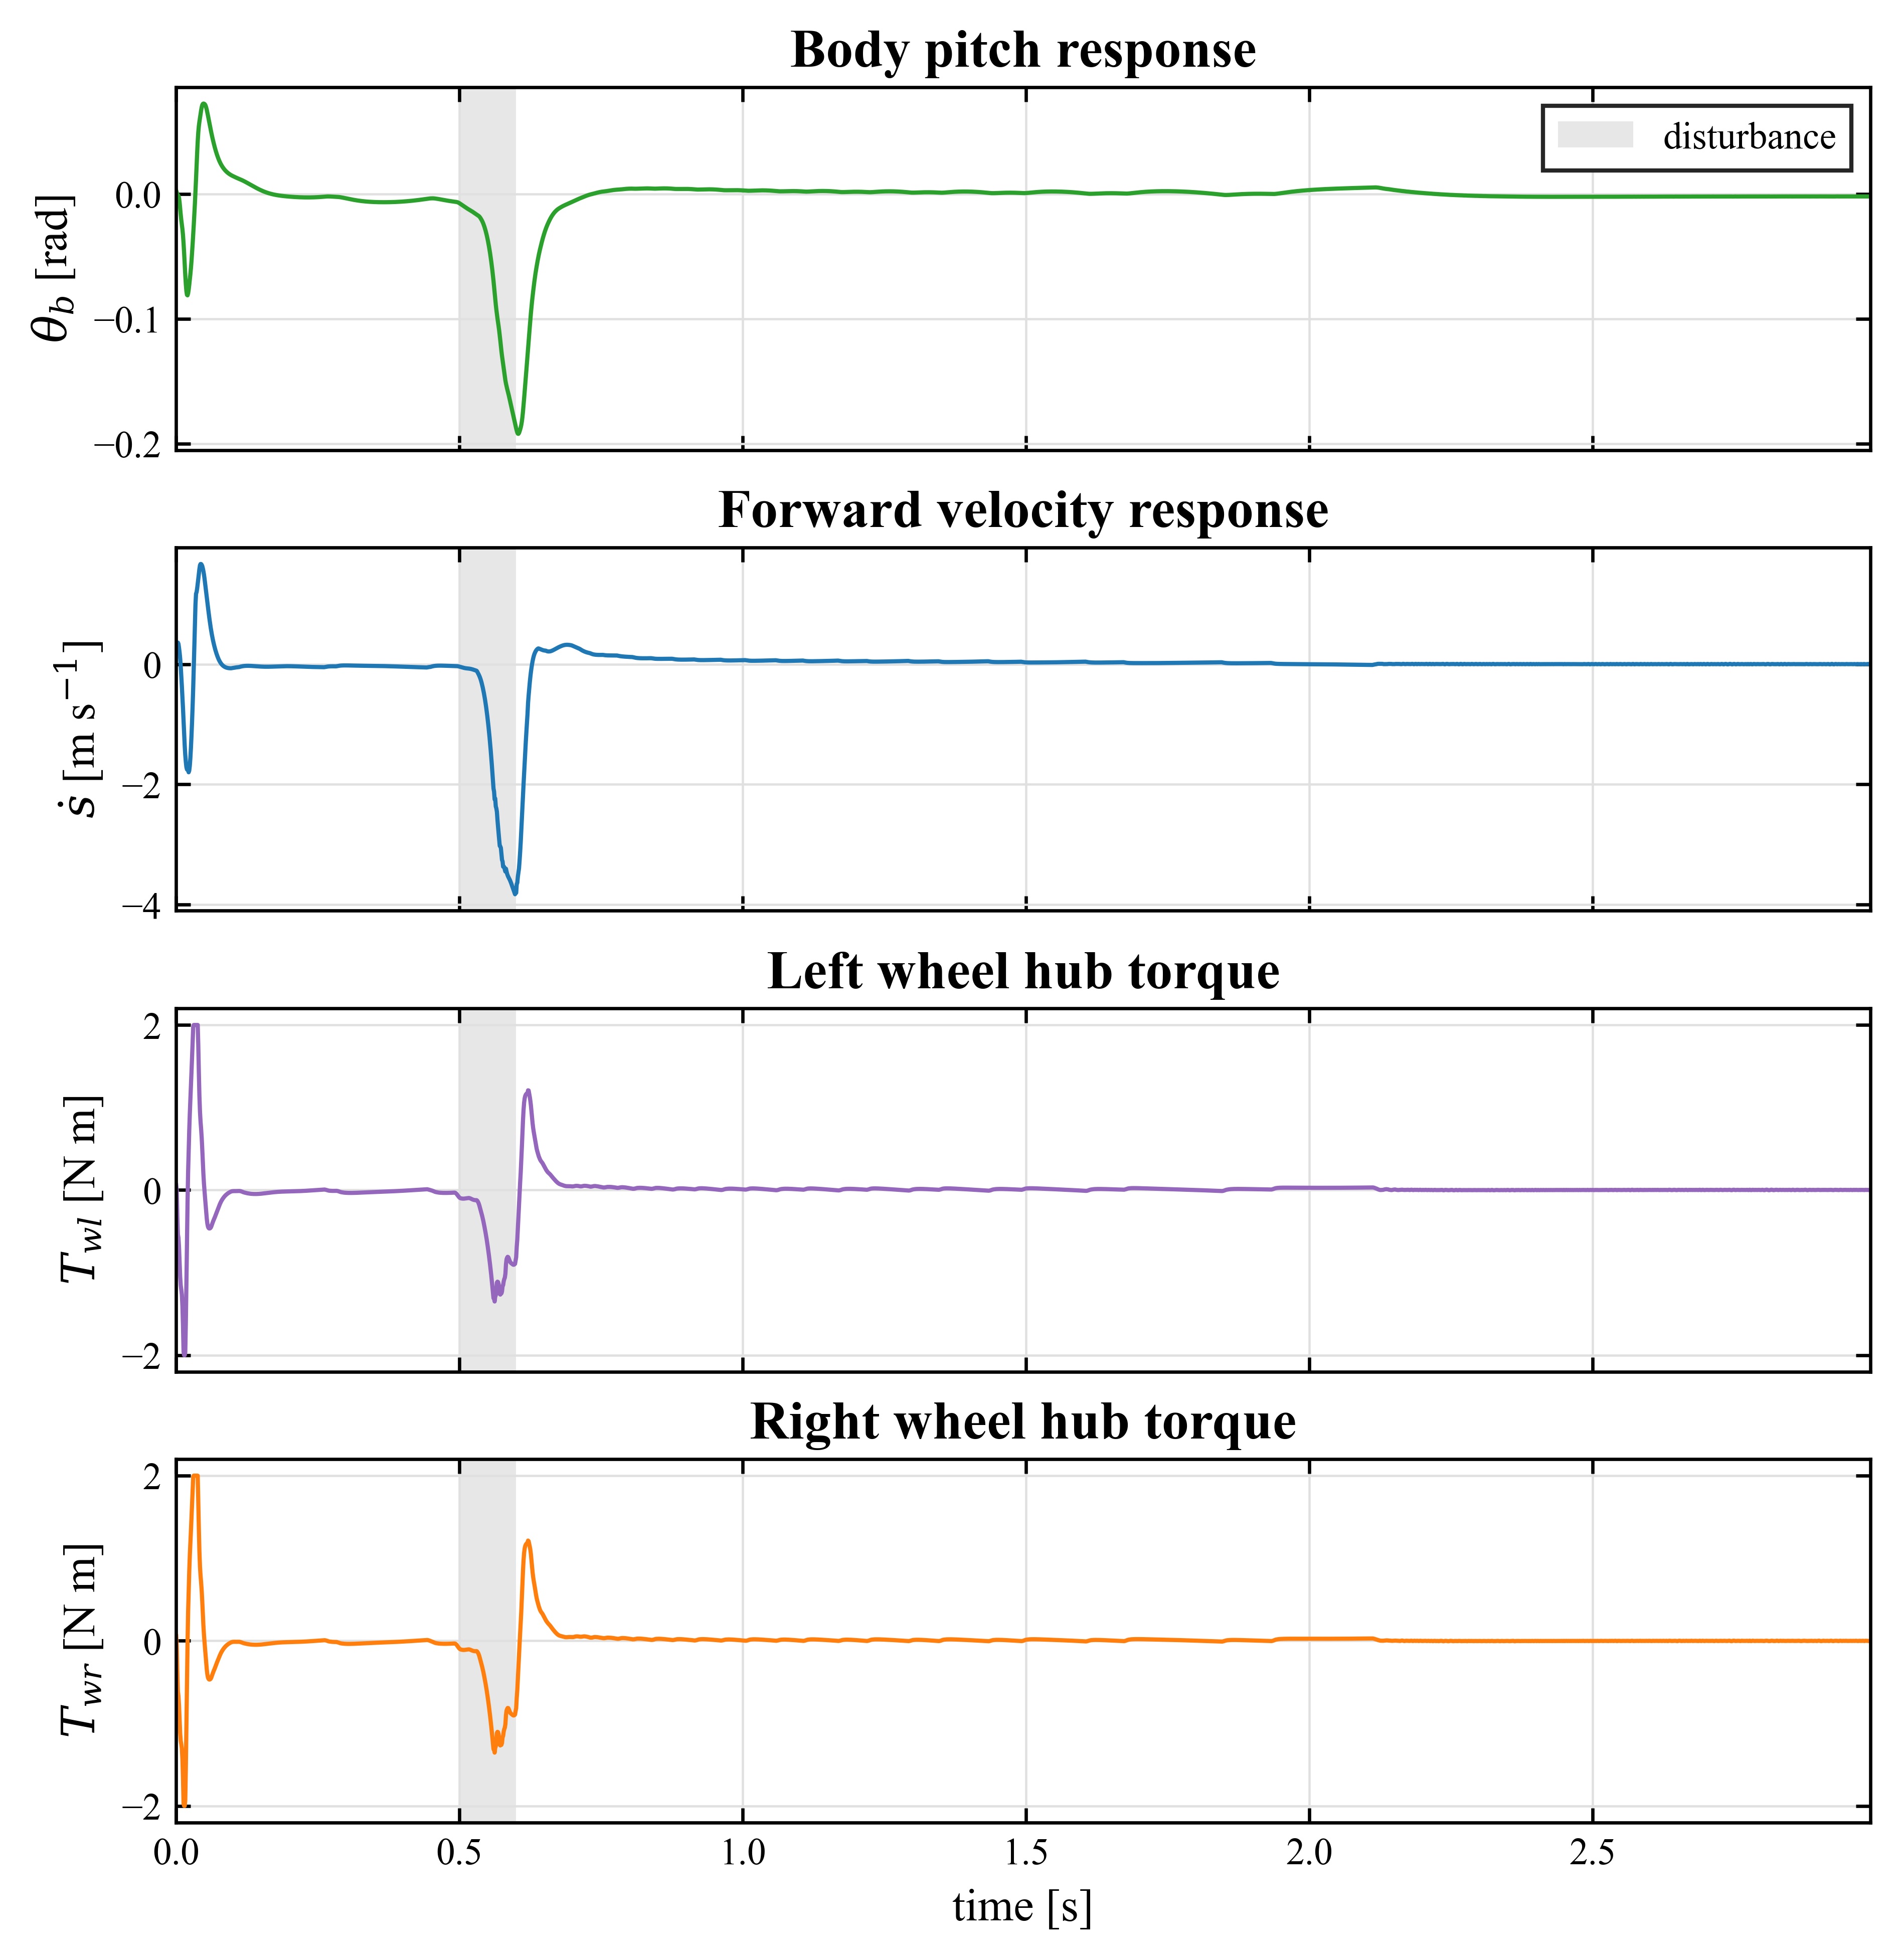
\includegraphics[width=\textwidth]{figures/ch04/vertical_impulse_out.png}
    \caption{竖直脉冲扰动响应}
    \label{fig:vertical-impulse-out}
  \end{subfigure}
  \hfill
  \begin{subfigure}[t]{0.49\textwidth}
    \centering
    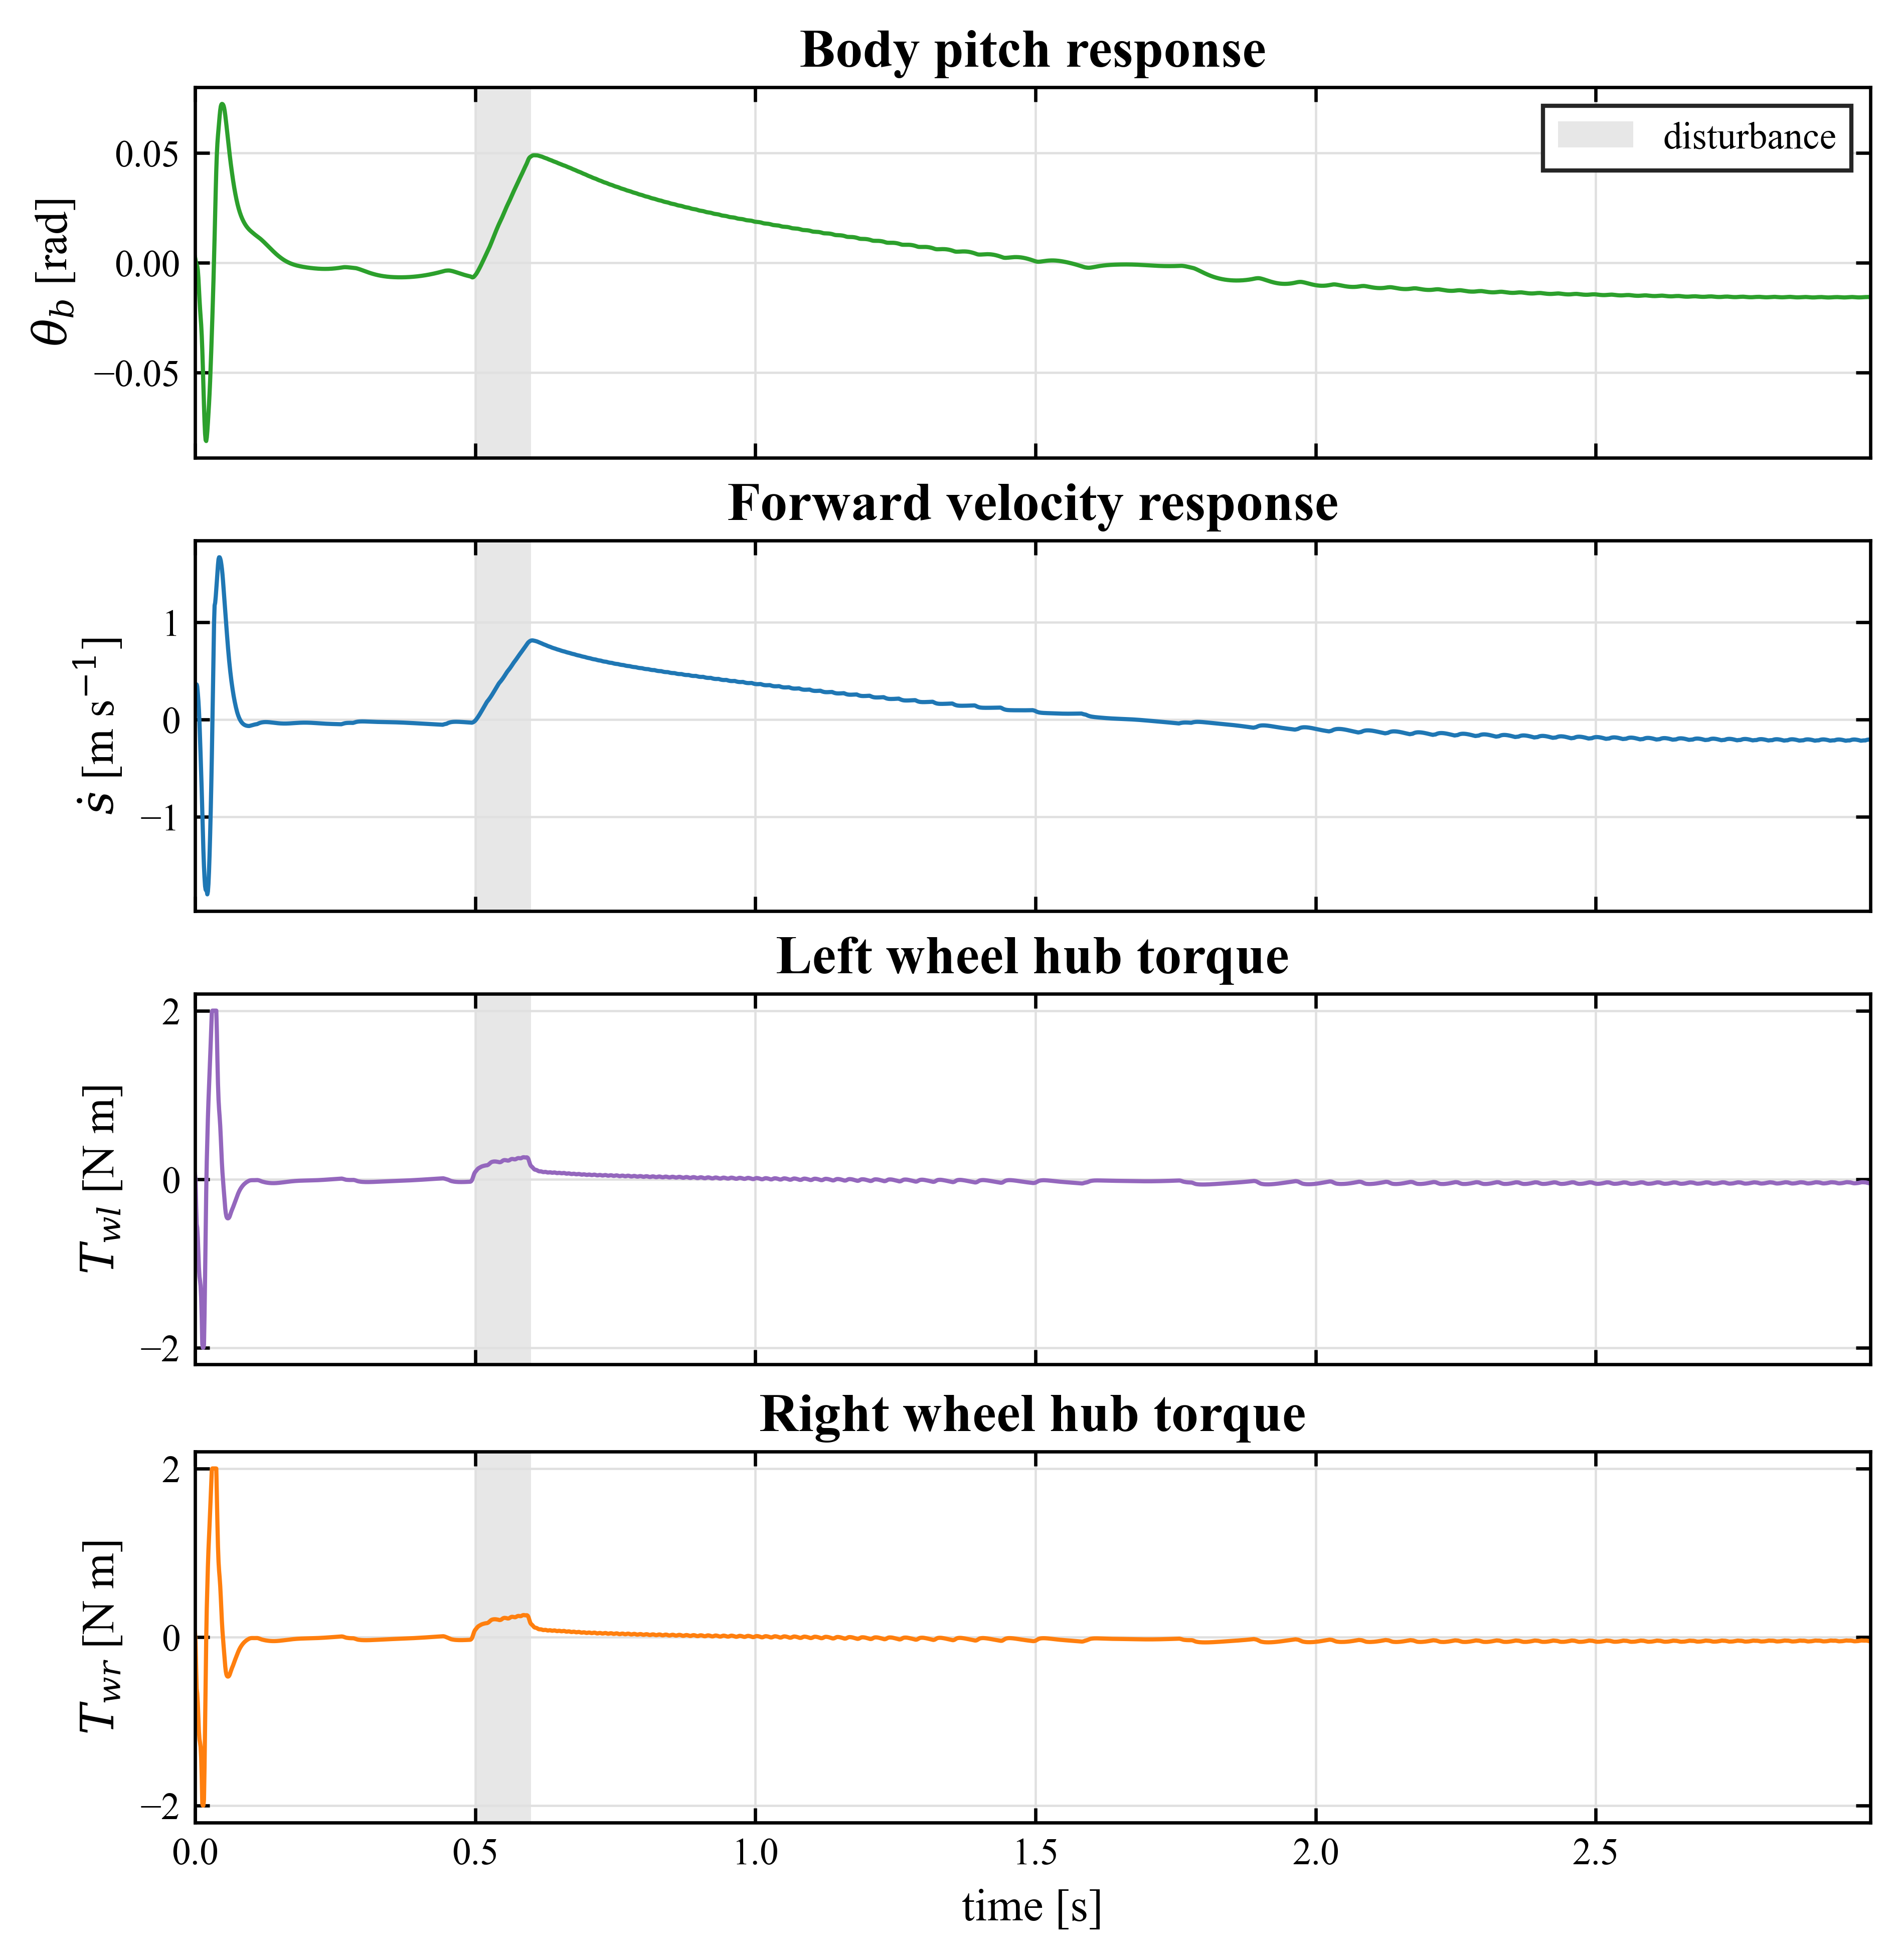
\includegraphics[width=\textwidth]{figures/ch04/horizon_impulse_out.png}
    \caption{水平脉冲扰动响应}
    \label{fig:horizon-impulse-out}
  \end{subfigure}
  \caption{不同方向脉冲扰动下的闭环响应}
  \label{fig:impulse-disturbance-out}
\end{figure}

由\figref{fig:vertical-impulse-out} 可见，竖直扰动施加后，腿部轴向力首先出现短时峰值，随后在阻尼项作用下逐渐回到稳定支撑范围，左右腿长也未产生持续发散。该结果说明 VMC 腿长通道能够对瞬时竖直载荷进行缓冲。由\figref{fig:horizon-impulse-out} 可见，水平扰动施加后，机体俯仰角和前进速度出现瞬时偏差，轮端力矩随即产生反向调节，使机器人重新回到平衡状态。两类扰动结果表明，本文控制器在不同方向外部冲击下均具有一定恢复能力。

\subsection{腿长控制验证}

腿长控制验证用于检查 VMC 腿长通道对不同期望腿长的响应能力。仿真中保持机器人处于原地平衡状态，前进速度参考取 $\dot{s}_d=0$，分别对左右腿公共期望腿长 $l_d$ 施加阶跃激励和正弦激励。阶跃激励用于观察腿长指令突变时的快速调节能力，正弦激励用于观察连续高度变化下的跟踪能力。两类工况能够直接反映式\eqref{eq:leg-force-law} 所构造的虚拟弹簧阻尼控制律是否能够驱动腿部机构完成高度调节，并检验腿长变化过程中机体俯仰角和腿部轴向力是否保持在合理范围内。

\begin{figure}[H]
  \centering
  \begin{subfigure}[t]{0.49\textwidth}
    \centering
    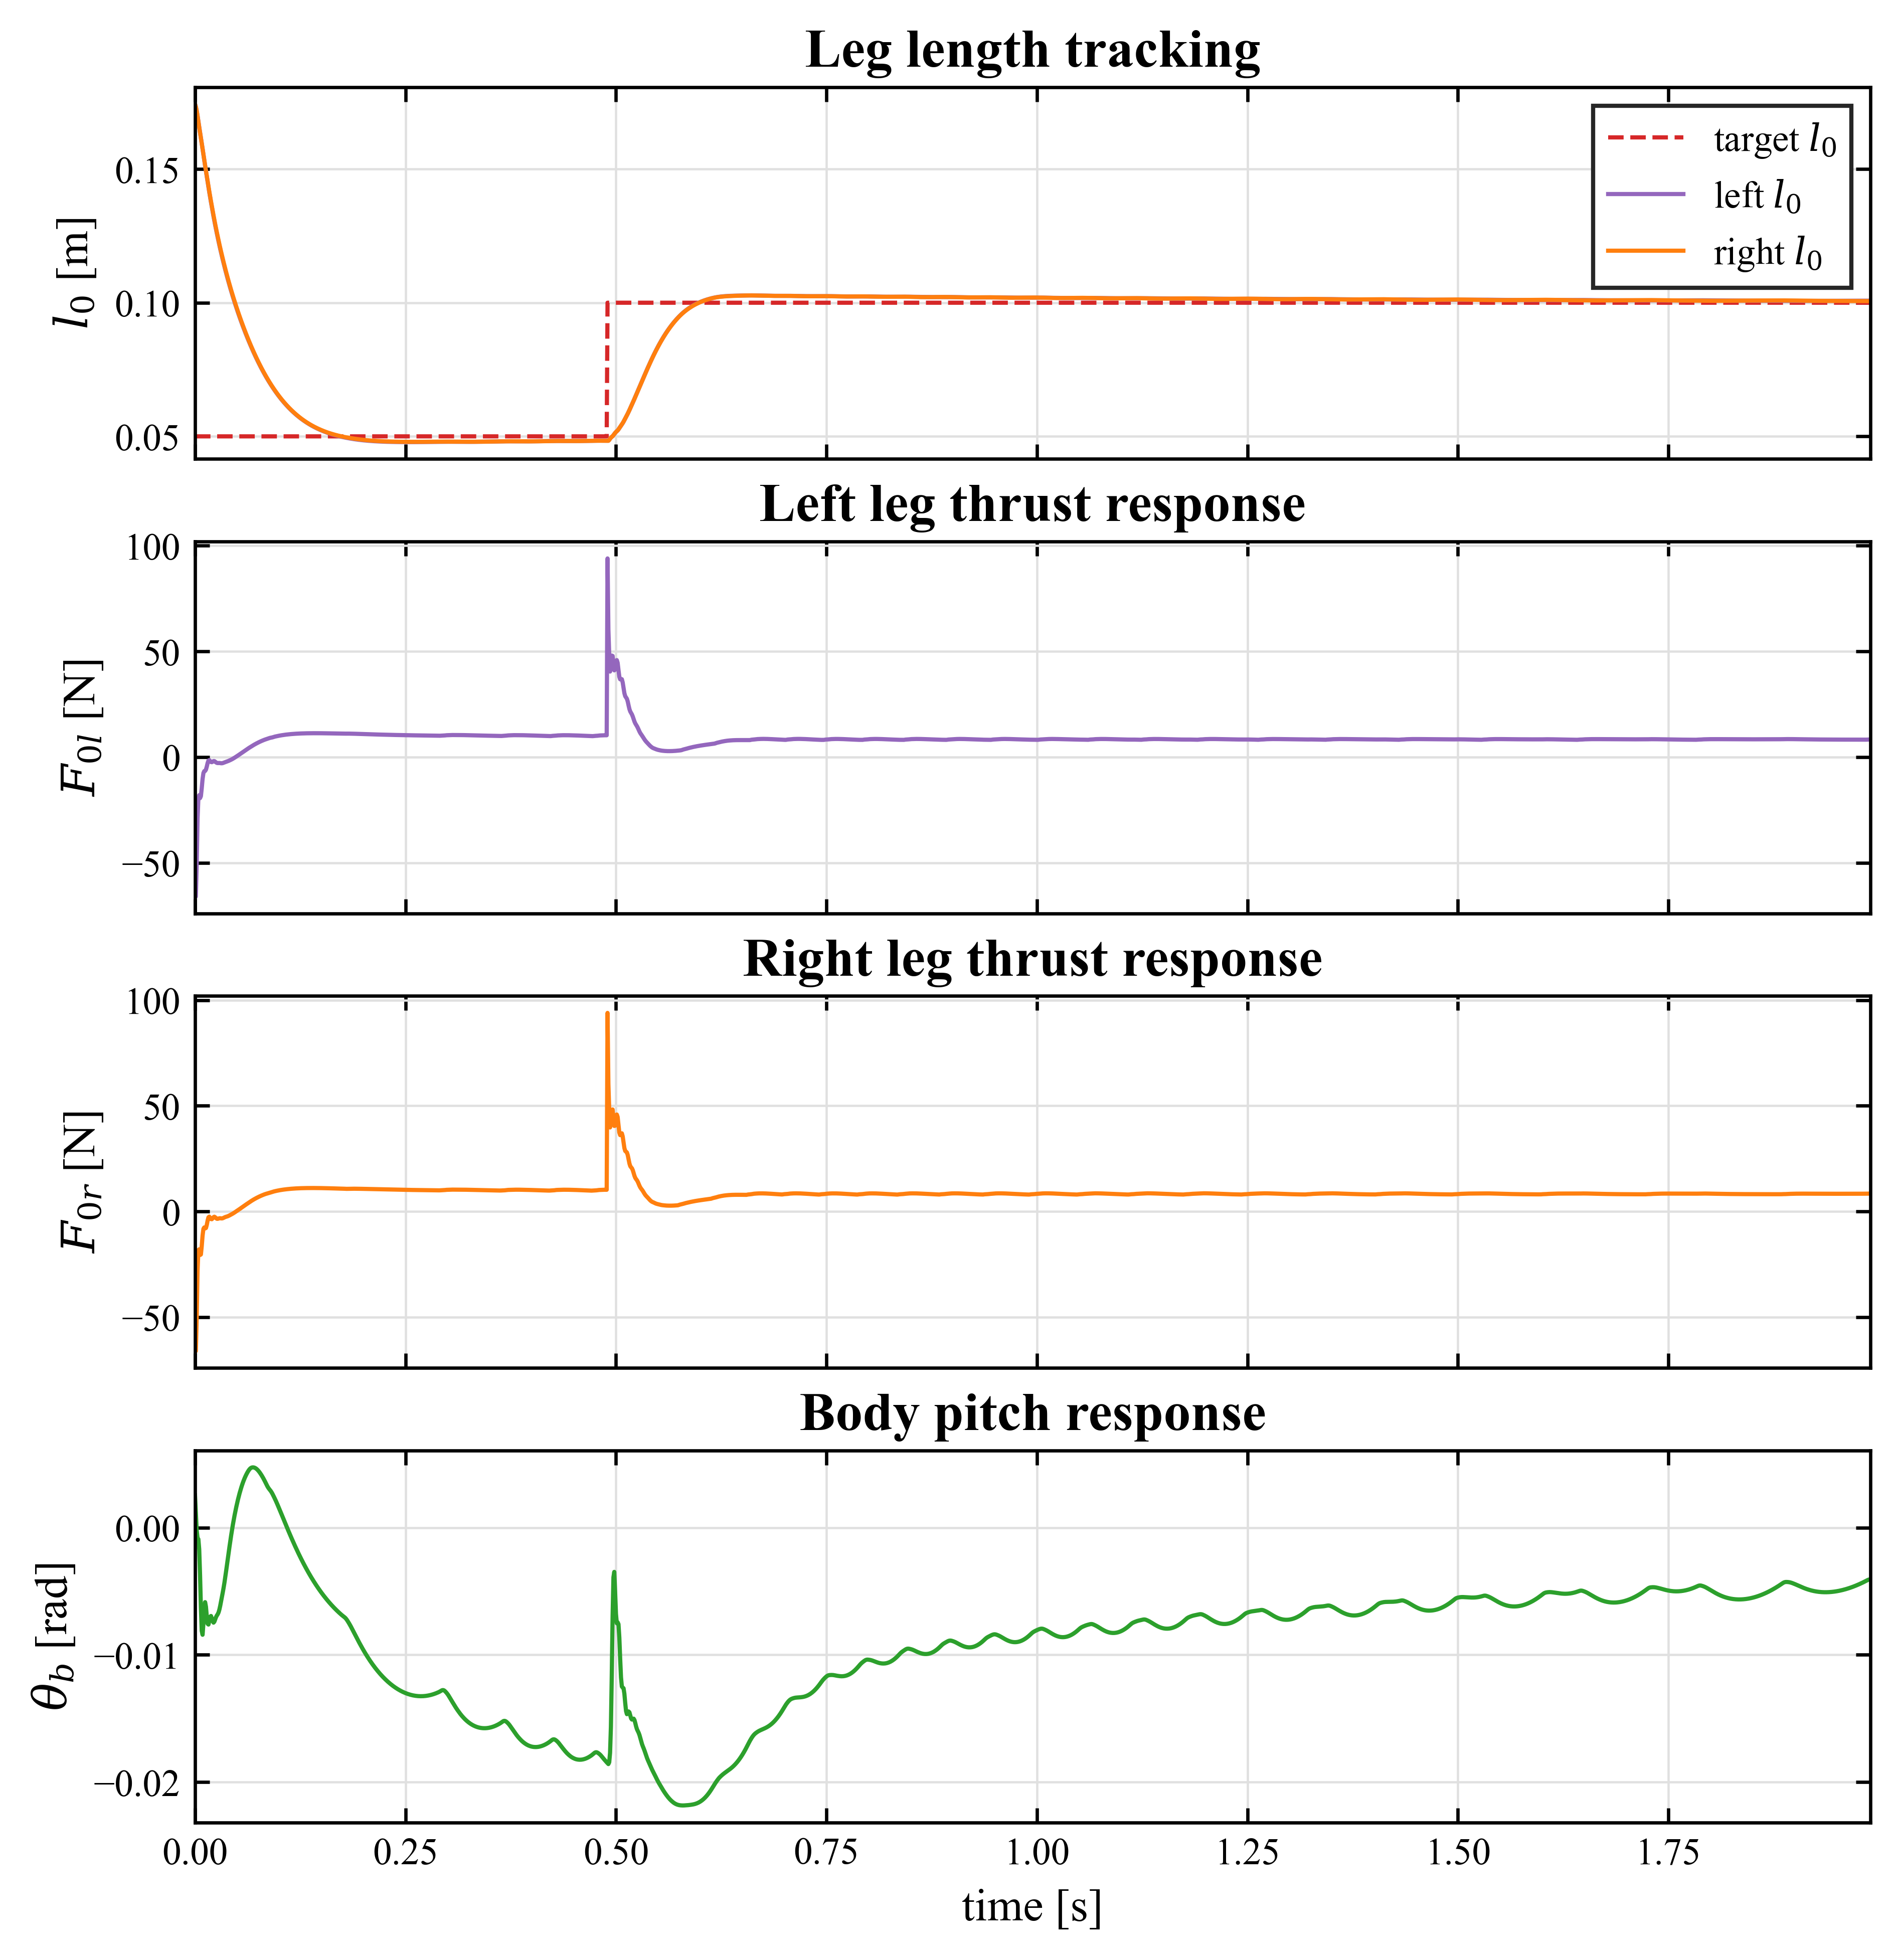
\includegraphics[width=\textwidth]{figures/ch04/step_velocity.png}
    \caption{阶跃腿长指令响应}
    \label{fig:leg-length-step}
  \end{subfigure}
  \hfill
  \begin{subfigure}[t]{0.49\textwidth}
    \centering
    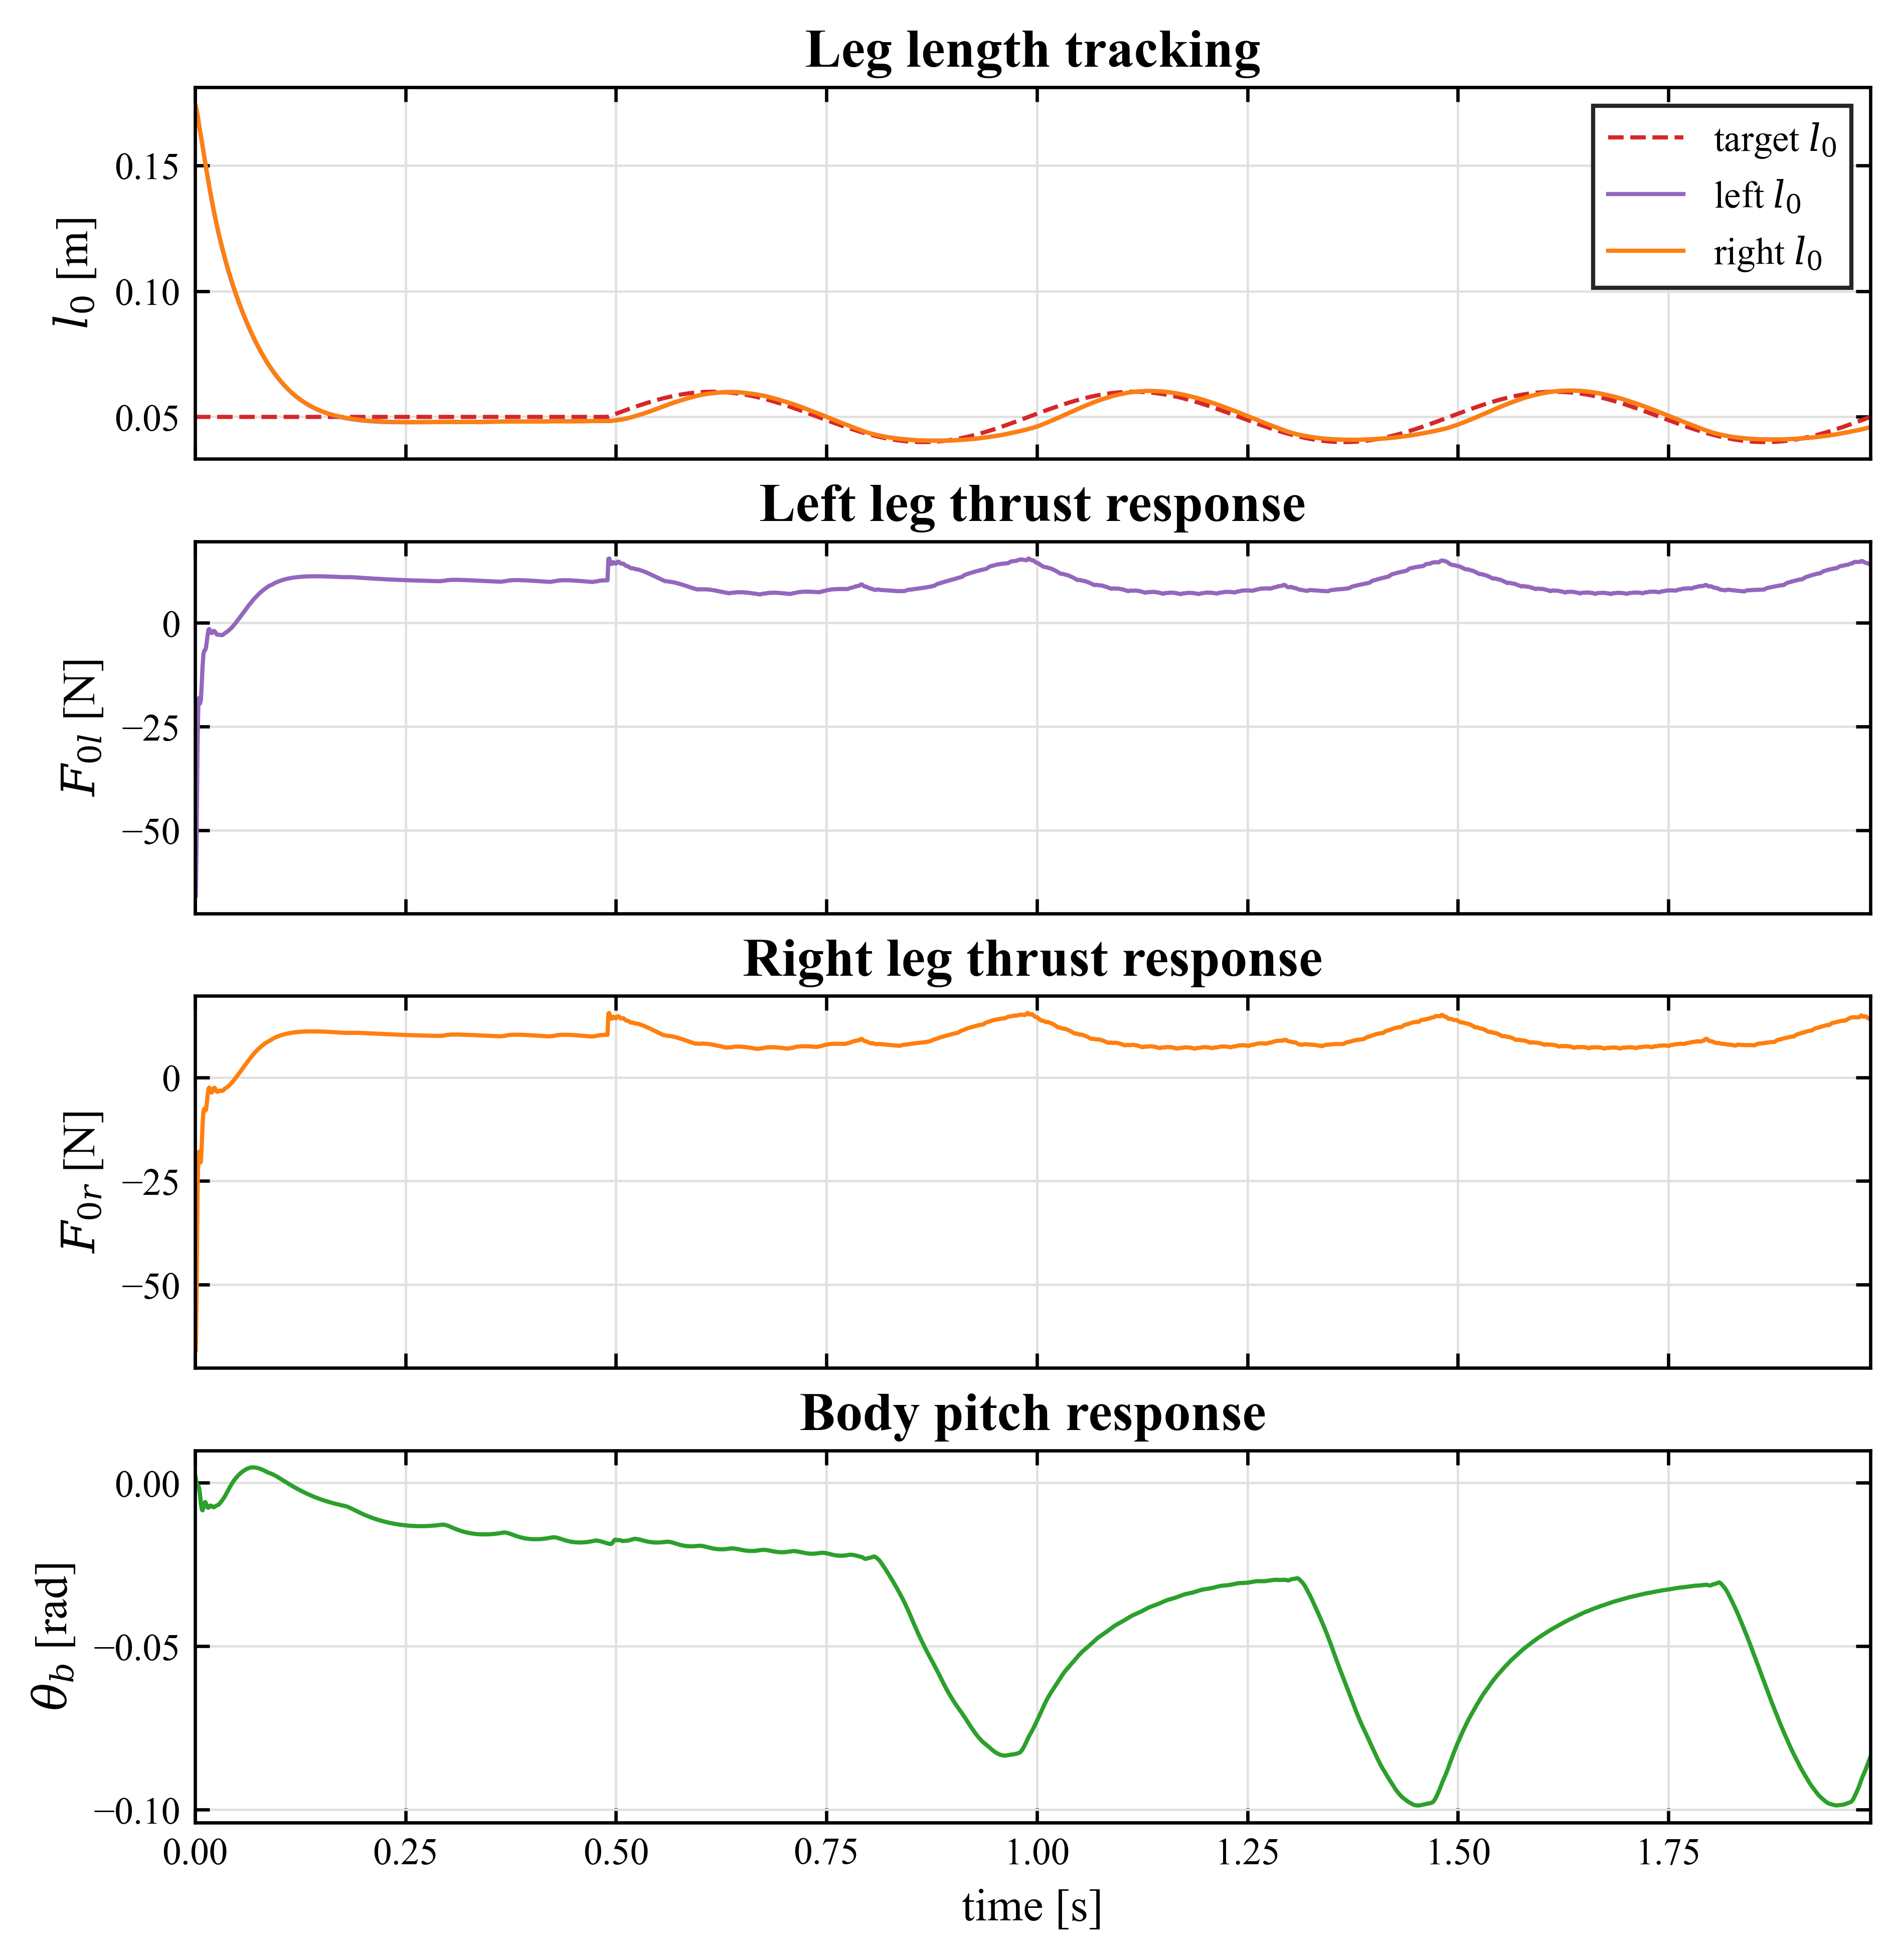
\includegraphics[width=\textwidth]{figures/ch04/sine_velocity.png}
    \caption{正弦腿长指令响应}
    \label{fig:leg-length-sine}
  \end{subfigure}
  \caption{不同腿长激励下的 VMC 腿长控制响应。从上至下分别为腿长跟踪、左腿轴向力、右腿轴向力和机体俯仰角}
  \label{fig:leg-length-excitation}
\end{figure}

由\figref{fig:leg-length-step} 可见，当期望腿长在 $0.5\,\mathrm{s}$ 附近由低位腿长切换至较高腿长时，左右腿实际腿长能够快速跟随参考值并在短时间内收敛。腿长突变瞬间，左右腿轴向力出现短时峰值，这是虚拟弹簧阻尼器为克服腿部惯性和支撑载荷而产生的瞬态输出；随后轴向力回到稳定支撑范围。机体俯仰角仅出现小幅波动，说明腿长阶跃调节未破坏整机平衡。

由\figref{fig:leg-length-sine} 可见，在正弦期望腿长输入下，左右腿实际腿长能够连续跟随目标曲线，虽然存在一定相位滞后，但整体变化趋势与参考信号一致。左右腿轴向力随期望腿长变化呈周期性调节，反映 VMC 控制器能够根据腿长误差持续修正支撑力。该结果说明本文腿长控制器不仅能够响应离散高度切换，也能够支持连续高度调节，为后续越障、缓冲和姿态调节动作提供了基础。

\section{本章小结}

本章围绕双轮足机器人控制系统的实际需求，提出了一种面向嵌入式实时实现的 LQR-VMC 平衡控制算法。
首先，从控制目标和工程约束出发，说明了采用“LQR 运动 + VMC 腿长支撑 + 滚转补偿”这一分层架构的原因；随后，基于第三章的建模结果构建了运动控制器所需的线性状态空间模型，并设计了 LQR 反馈律；在此基础上，通过 VMC 完成腿长支撑控制，并将 LQR 输出的腿摆控制量一并映射到关节空间，同时利用滚转辅助控制实现左右腿长参考修正；最后，给出了控制系统的状态估计与在线工作流程，并说明了 MuJoCo 仿真验证的模型构建、工况设置和数据记录方法。上述内容共同构成了本文后续物理样机实验所依赖的控制系统实现基础。

\chapter{物理样机实验验证}\label{chap:experiment}

本章在物理样机上对第四章的控制方案进行验证，按原地平衡、速度跟踪、腿长控制和滚转稳定四个工况依次展开。记录的数据包括机体俯仰角 $\theta_b$、滚转角 $\gamma$、前进速度 $\dot{s}$、左右虚拟腿长 $l_l,l_r$、轮端力矩 $T_{lw,l},T_{lw,r}$ 和腿部关节力矩 $\tau_l,\tau_r$。俯仰角和速度用来评估 LQR 的平衡与跟踪表现，腿长及关节力矩用来检查 VMC 腿长通道的实际支撑效果，滚转角和腿长差用来判断侧向补偿是否起作用。
\section{物理样机平台介绍}

实验样机由机械本体、驱动系统、传感系统、嵌入式控制系统和上位机记录系统组成。机械部分沿用第二章提出的混合式双轮足结构，左右腿均采用对称闭环连杆机构，足端安装轮毂电机。腿部关节电机布置在靠近躯干的位置，并通过链传动驱动连杆运动，从而在保证腿部运动范围的同时减小末端转动惯量。

\begin{figure}[H]
  \centering
  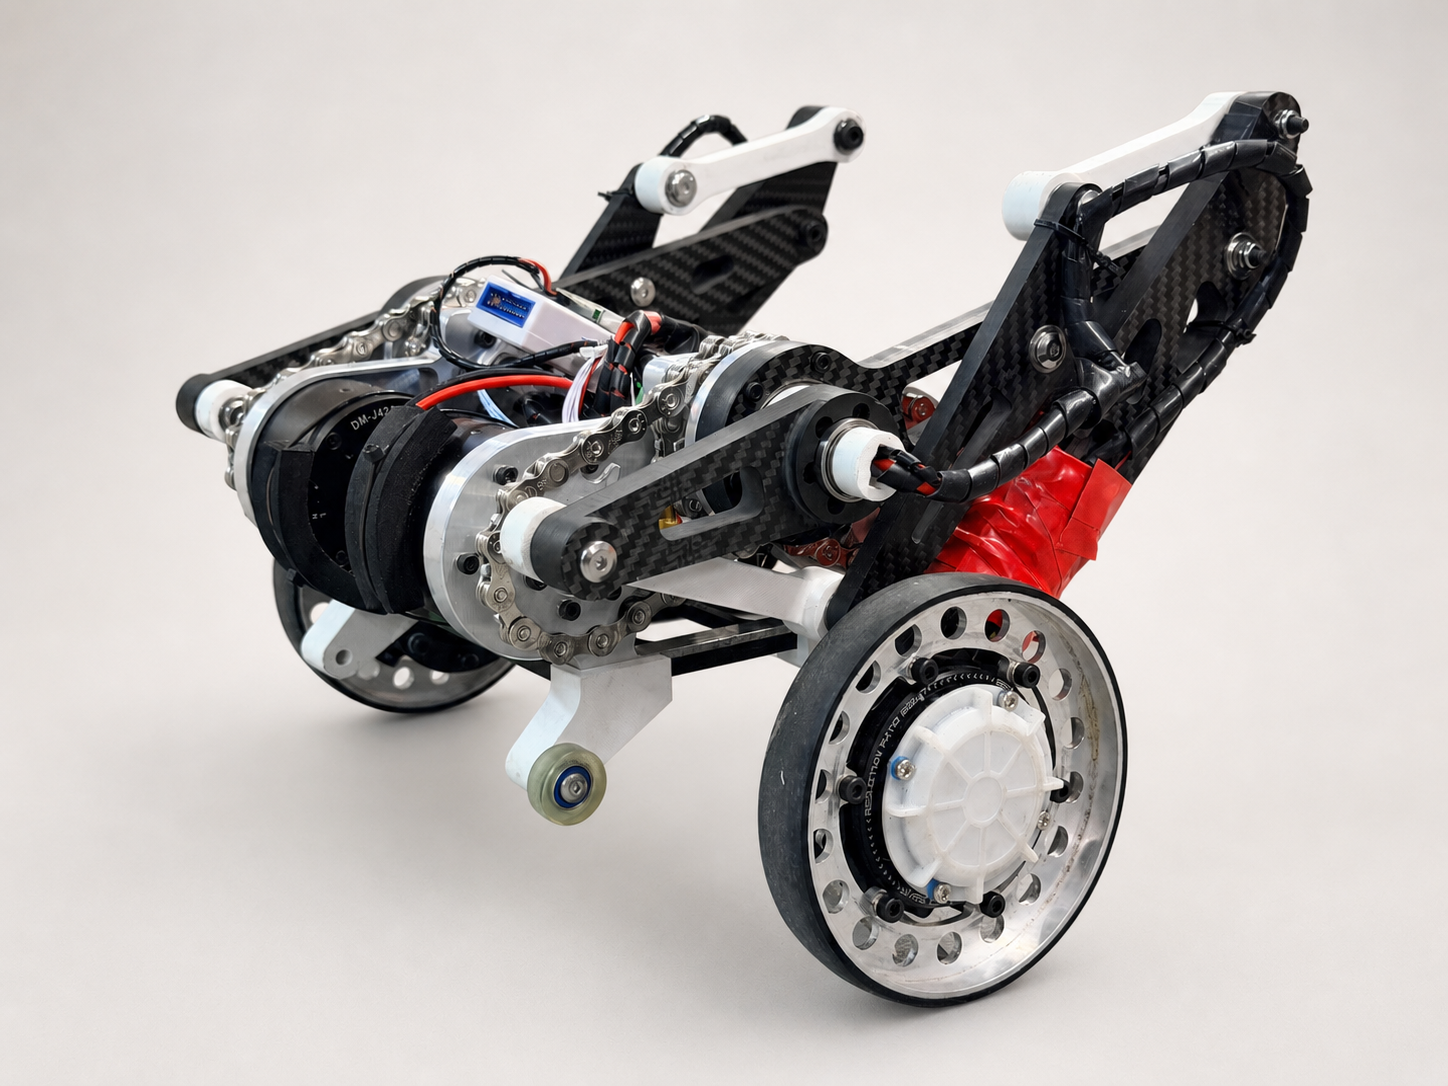
\includegraphics[width=0.85\textwidth]{figures/ch05/demo.png}
  \caption{物理样机实物图}
\end{figure}

控制程序部署在 STM32H723 主控板上，主频为 $480\,\mathrm{MHz}$。每个控制周期内，主控板读取惯性测量单元、轮毂电机编码器和腿部关节编码器的数据，并按照第四章的状态估计方法更新机体姿态、前进速度、虚拟腿长和腿摆角。随后，程序计算 LQR 输出的轮端力矩与腿摆控制量、VMC 输出的腿长支撑力以及滚转修正量，再将对应力矩指令发送给各电机驱动器。

传感器布置与状态估计量一一对应。惯性测量单元安装在机体中部附近，直接给出俯仰角、滚转角及角速度；轮毂电机编码器提供左右轮角速度，并参与前进速度估计；腿部关节编码器结合第三章的五连杆运动学关系，解算左右虚拟腿长和腿摆角。实验数据由上位机通过无线烧录器记录，实验结束后再离线绘图和分析。

\begin{figure}[H]
  \centering
  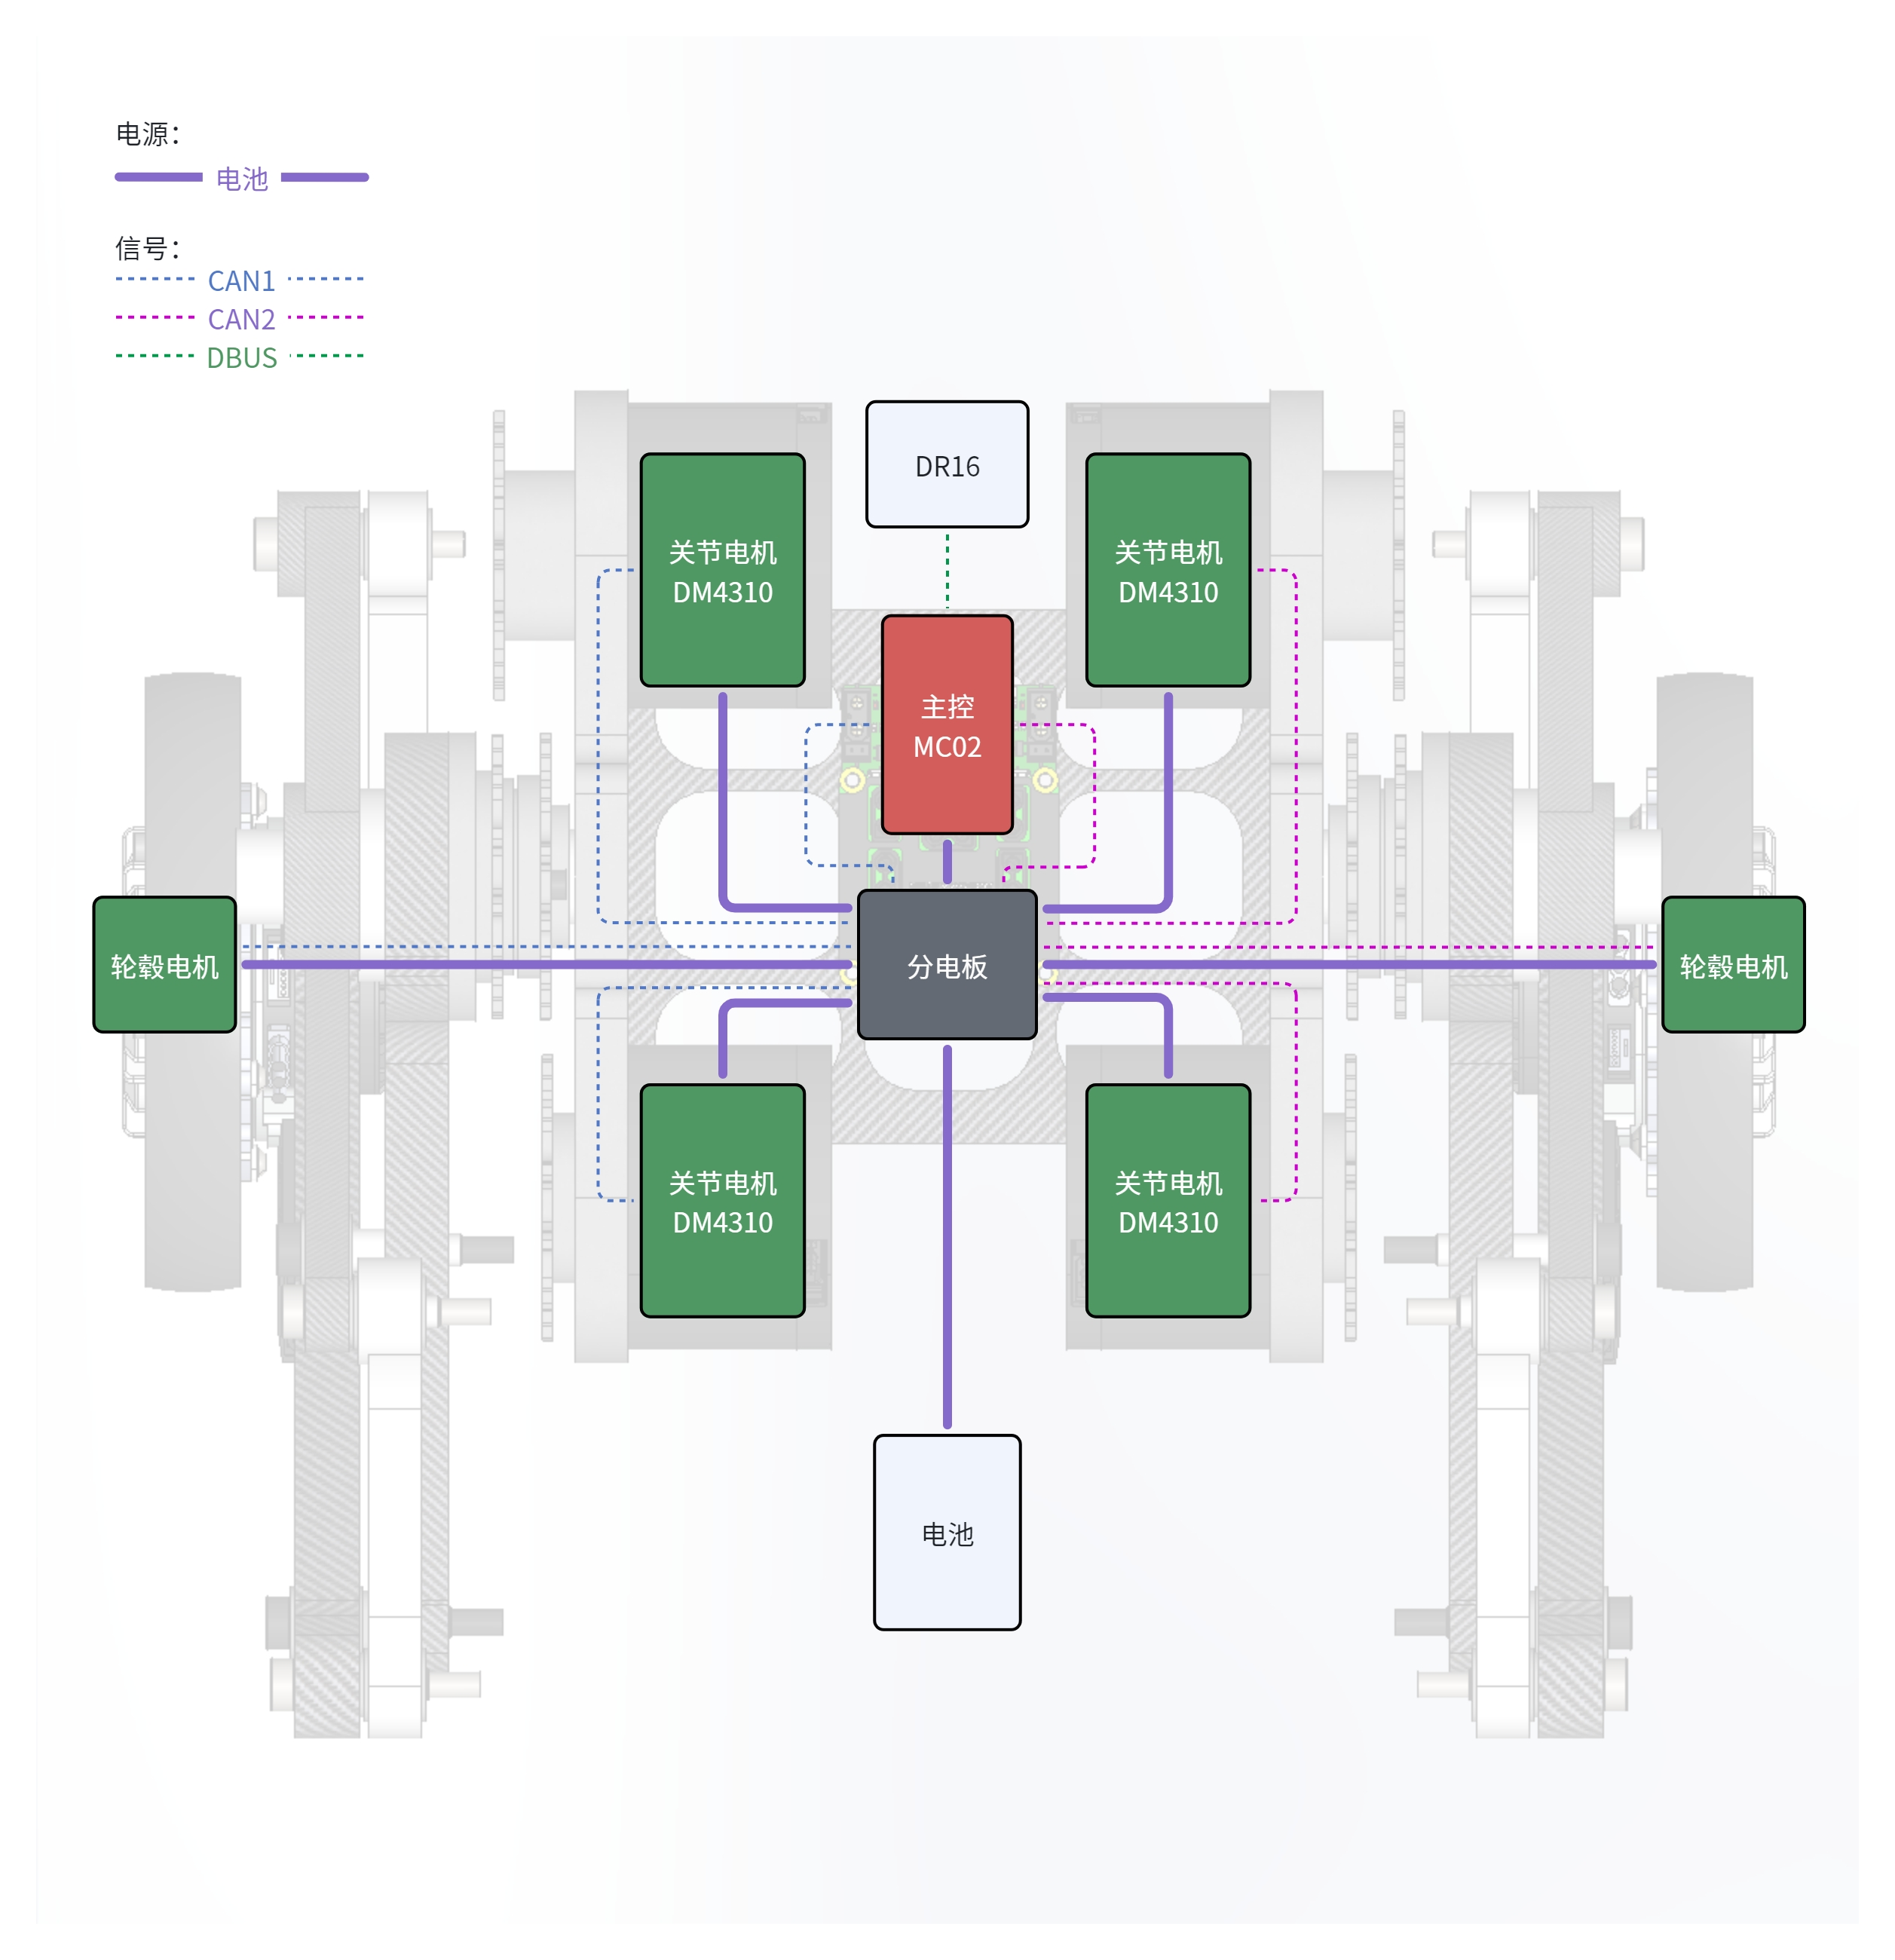
\includegraphics[width=0.7\textwidth]{figures/ch05/line.jpg}
  \caption{样机接线图}
  \label{fig:experiment-hardware}
\end{figure}

样机平台的主要参数见\tabref{tab:prototype-parameters}。这些参数与第二章的结构设计和执行器选型保持一致，是后续控制参数配置和实验结果分析的硬件基础。

\begin{table}[H]
  \centering
  \caption{物理样机主要参数}\label{tab:prototype-parameters}
  \renewcommand{\arraystretch}{1.25}
  \begin{tabular}{lcc}
    \toprule
    参数 & 数值 & 说明 \\
    \midrule
    整机质量 & 约 $3.5\,\mathrm{kg}$ & 含电池、控制板和驱动器 \\
    轮半径 & $0.06\,\mathrm{m}$ & 足端驱动轮半径 \\
    单腿主动自由度 & $2$ & 闭环连杆机构主动关节 \\
    轮端驱动自由度 & $2$ & 左右轮毂电机差速驱动 \\
    腿部关节电机峰值扭矩 & $7\,\mathrm{N\cdot m}$ & 短时输出能力 \\
    轮毂电机额定扭矩 & $2.46\,\mathrm{N\cdot m}$ & 减速箱输出端 \\
    控制频率 & $1\,\mathrm{kHz}$ & 控制器目标运行频率 \\
    \bottomrule
  \end{tabular}
\end{table}

实物实验的控制结构与仿真一致：LQR 出轮端力矩和腿摆量，VMC 出腿长支撑力，滚转环出左右腿长差修正。不同的是，实物上多了执行器带宽、轮地接触状态和传感器噪声这些仿真里吃不透的因素。所以仿真参数只能当起点，实物上还得根据实际响应再调——有的增益要收，有的限幅要放，有的方向需要反复试。

调试的基本顺序是：先离线算好 LQR 增益，把轮端限幅压到较低水平，在保护架里做小幅站立；等机器人能从不大的初始偏斜里自己回来，再逐步放开轮端力矩限幅和姿态增益。主平衡站稳后，调 VMC 的刚度 $K_l$ 和阻尼 $D_l$，原则是腿撑得住、不振荡。滚转环最后接入，腿长差修正量设一个较小的上限，避免滚转角测量噪声引起左右腿高频哆嗦。

所有实验均在平整地面上完成。每组工况重复测试多次，离线分析时剔除通信中断、保护架碰撞、轮端离地等异常片段。本文主要从以下指标观察实验结果：

\begin{enumerate}
  \item 原地平衡实验：观察机体俯仰角和腿摆角是否收敛，前进速度是否快速收敛，以及轮端力矩是否出现长期饱和；
  \item 速度跟踪实验：观察实际速度相对参考速度的响应滞后、稳态误差和超调情况，同时检查速度变化过程中机体姿态是否保持稳定；
  \item 滚转稳定实验：观察滚转角峰值、恢复过程和左右腿长参考差异，分析滚转稳定对侧向姿态的改善作用；
  \item 腿长控制实验：观察左右实际腿长对参考腿长的跟踪能力、两侧响应一致性以及高度变化对整机平衡的影响。
\end{enumerate}

\section{原地平衡性能验证}

原地平衡是双轮足机器人开展其他运动实验的基础。实验中，左右腿参考长度均设为基准腿长，期望前进速度取 $\dot{s}_d=0$，偏航角和腿摆角参考值取零。样机由初始支撑状态进入直立状态后，LQR 控制器根据俯仰角、俯仰角速度和轮系状态输出轮端力矩，使机器人通过小范围前后移动维持倒立摆平衡；VMC 控制器则维持左右腿长在基准值附近，为机体提供稳定支撑。

\begin{figure}[H]
  \centering
  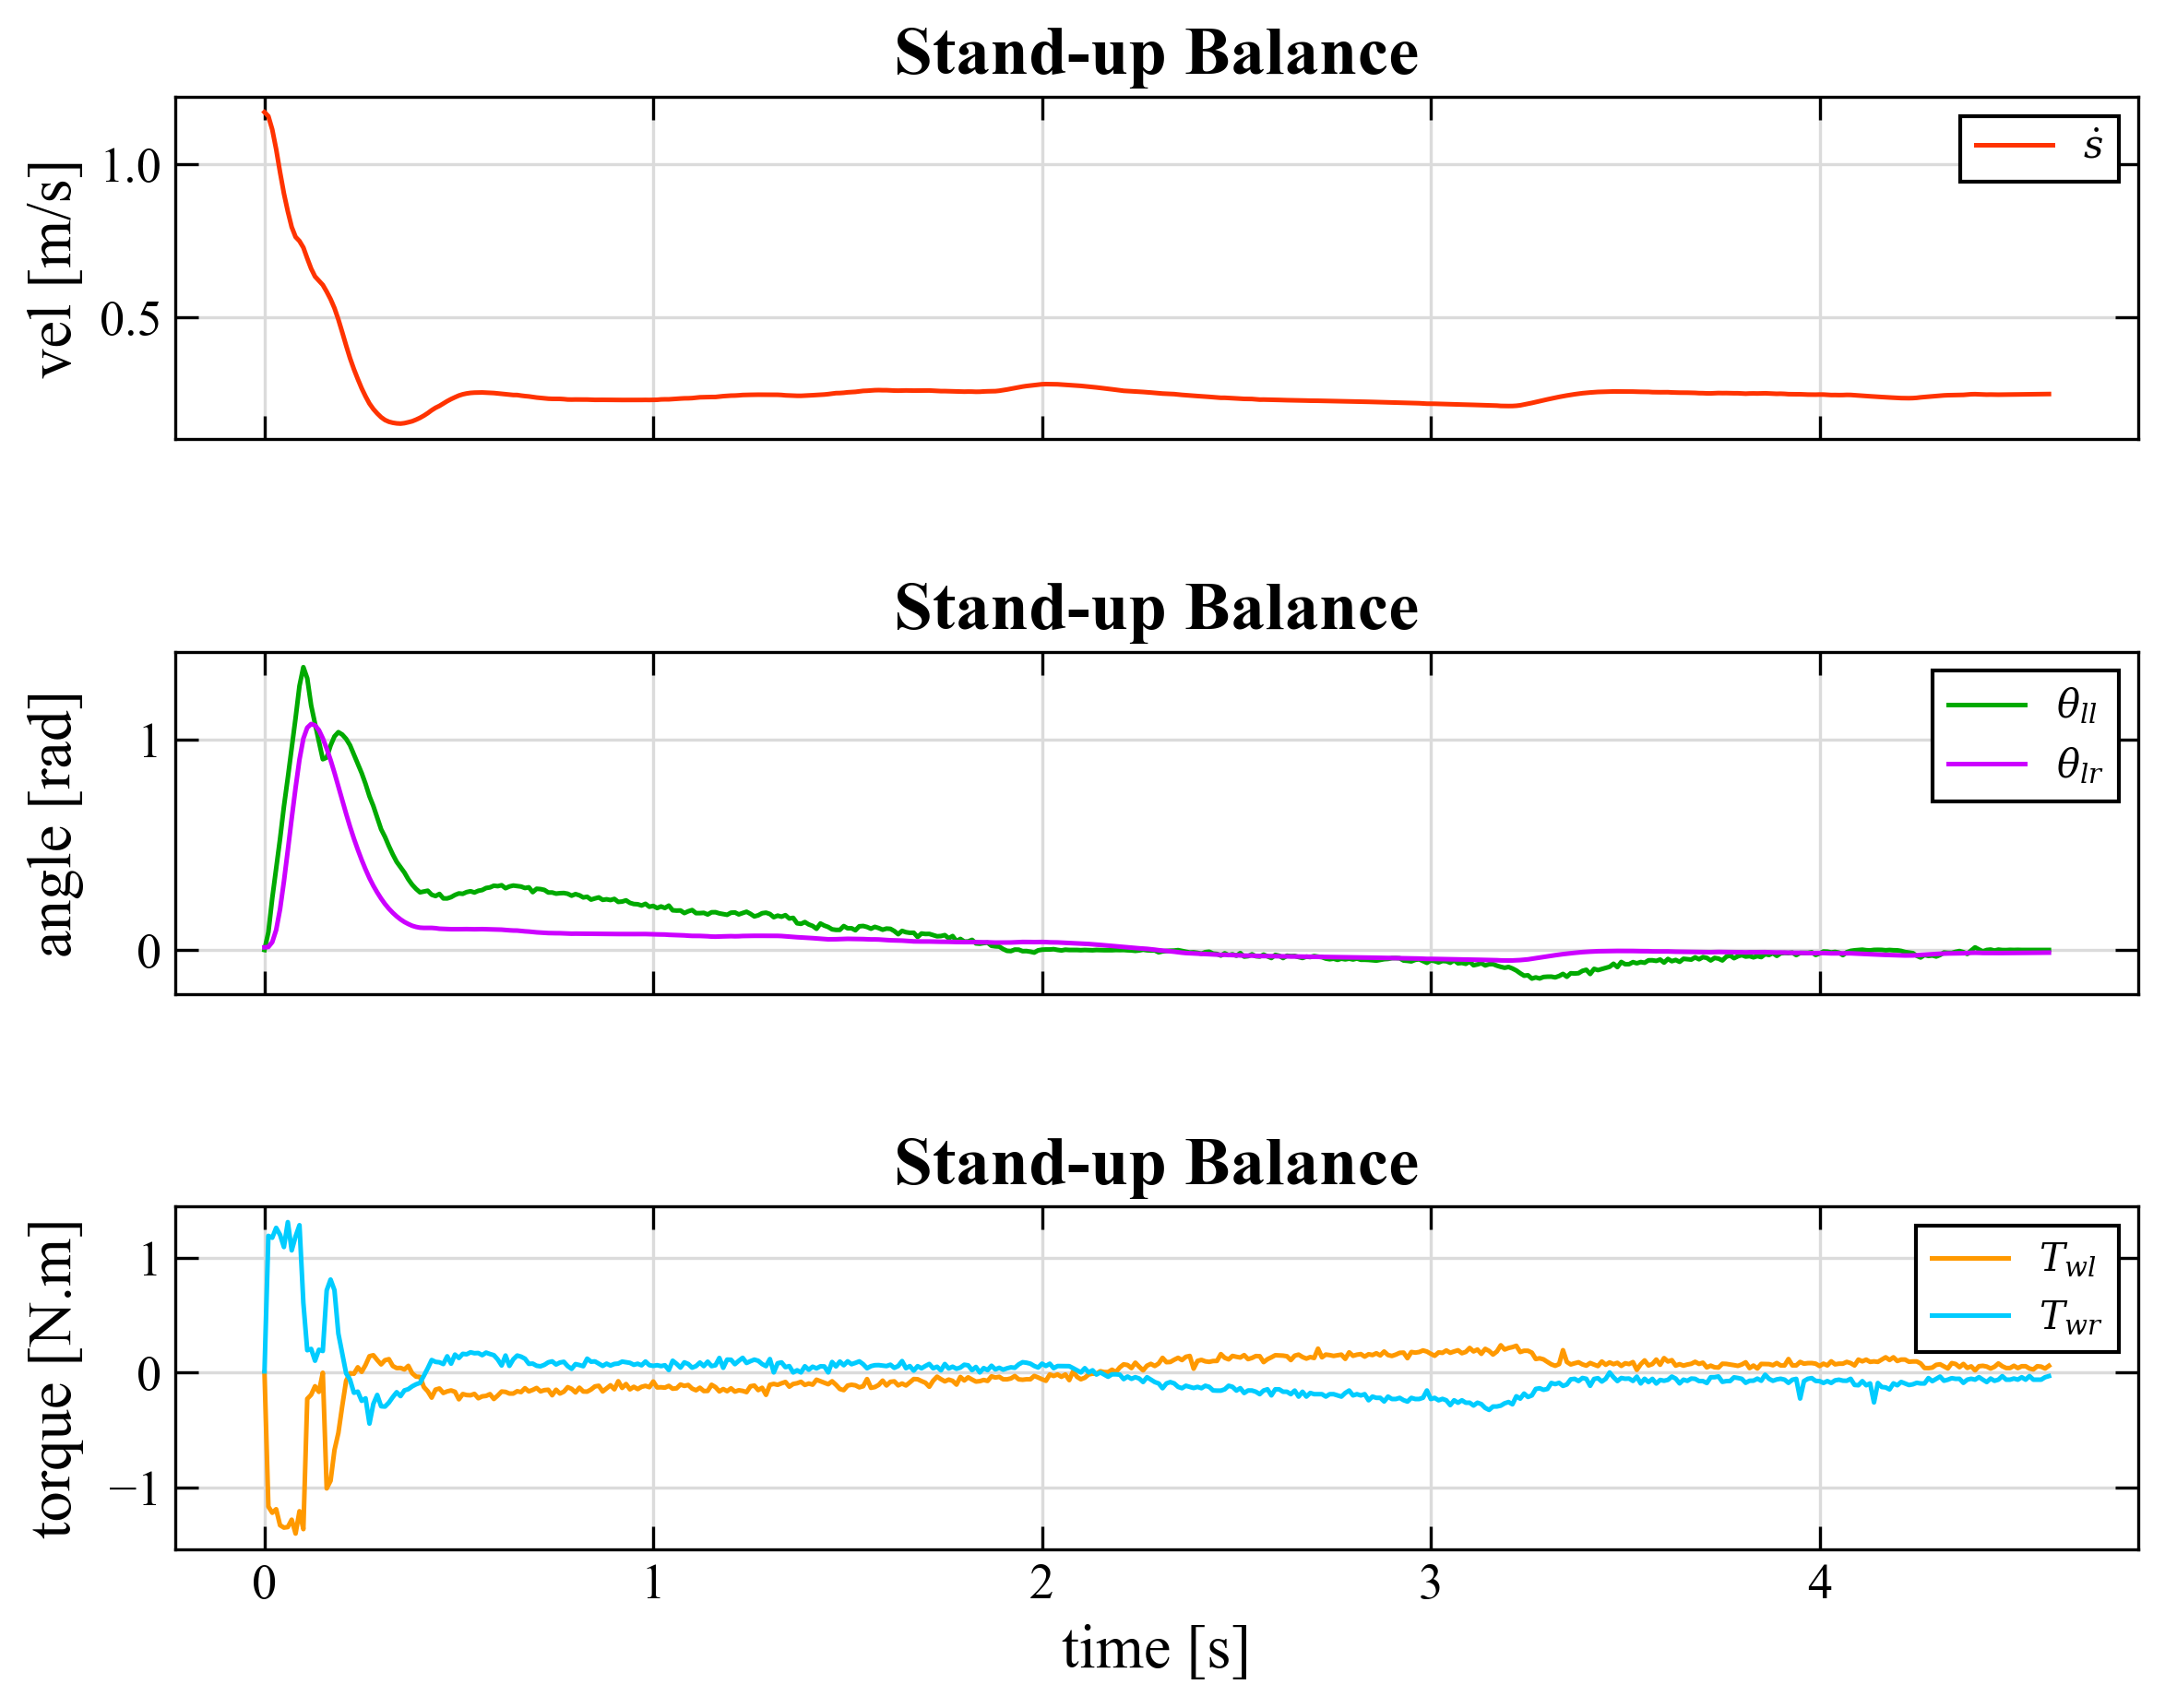
\includegraphics[width=1.0\textwidth]{figures/ch05/standup.png}
  \caption{原地平衡实验响应曲线}
  \label{fig:balance-experiment-response}
\end{figure}

\begin{figure}[H]
  \centering
  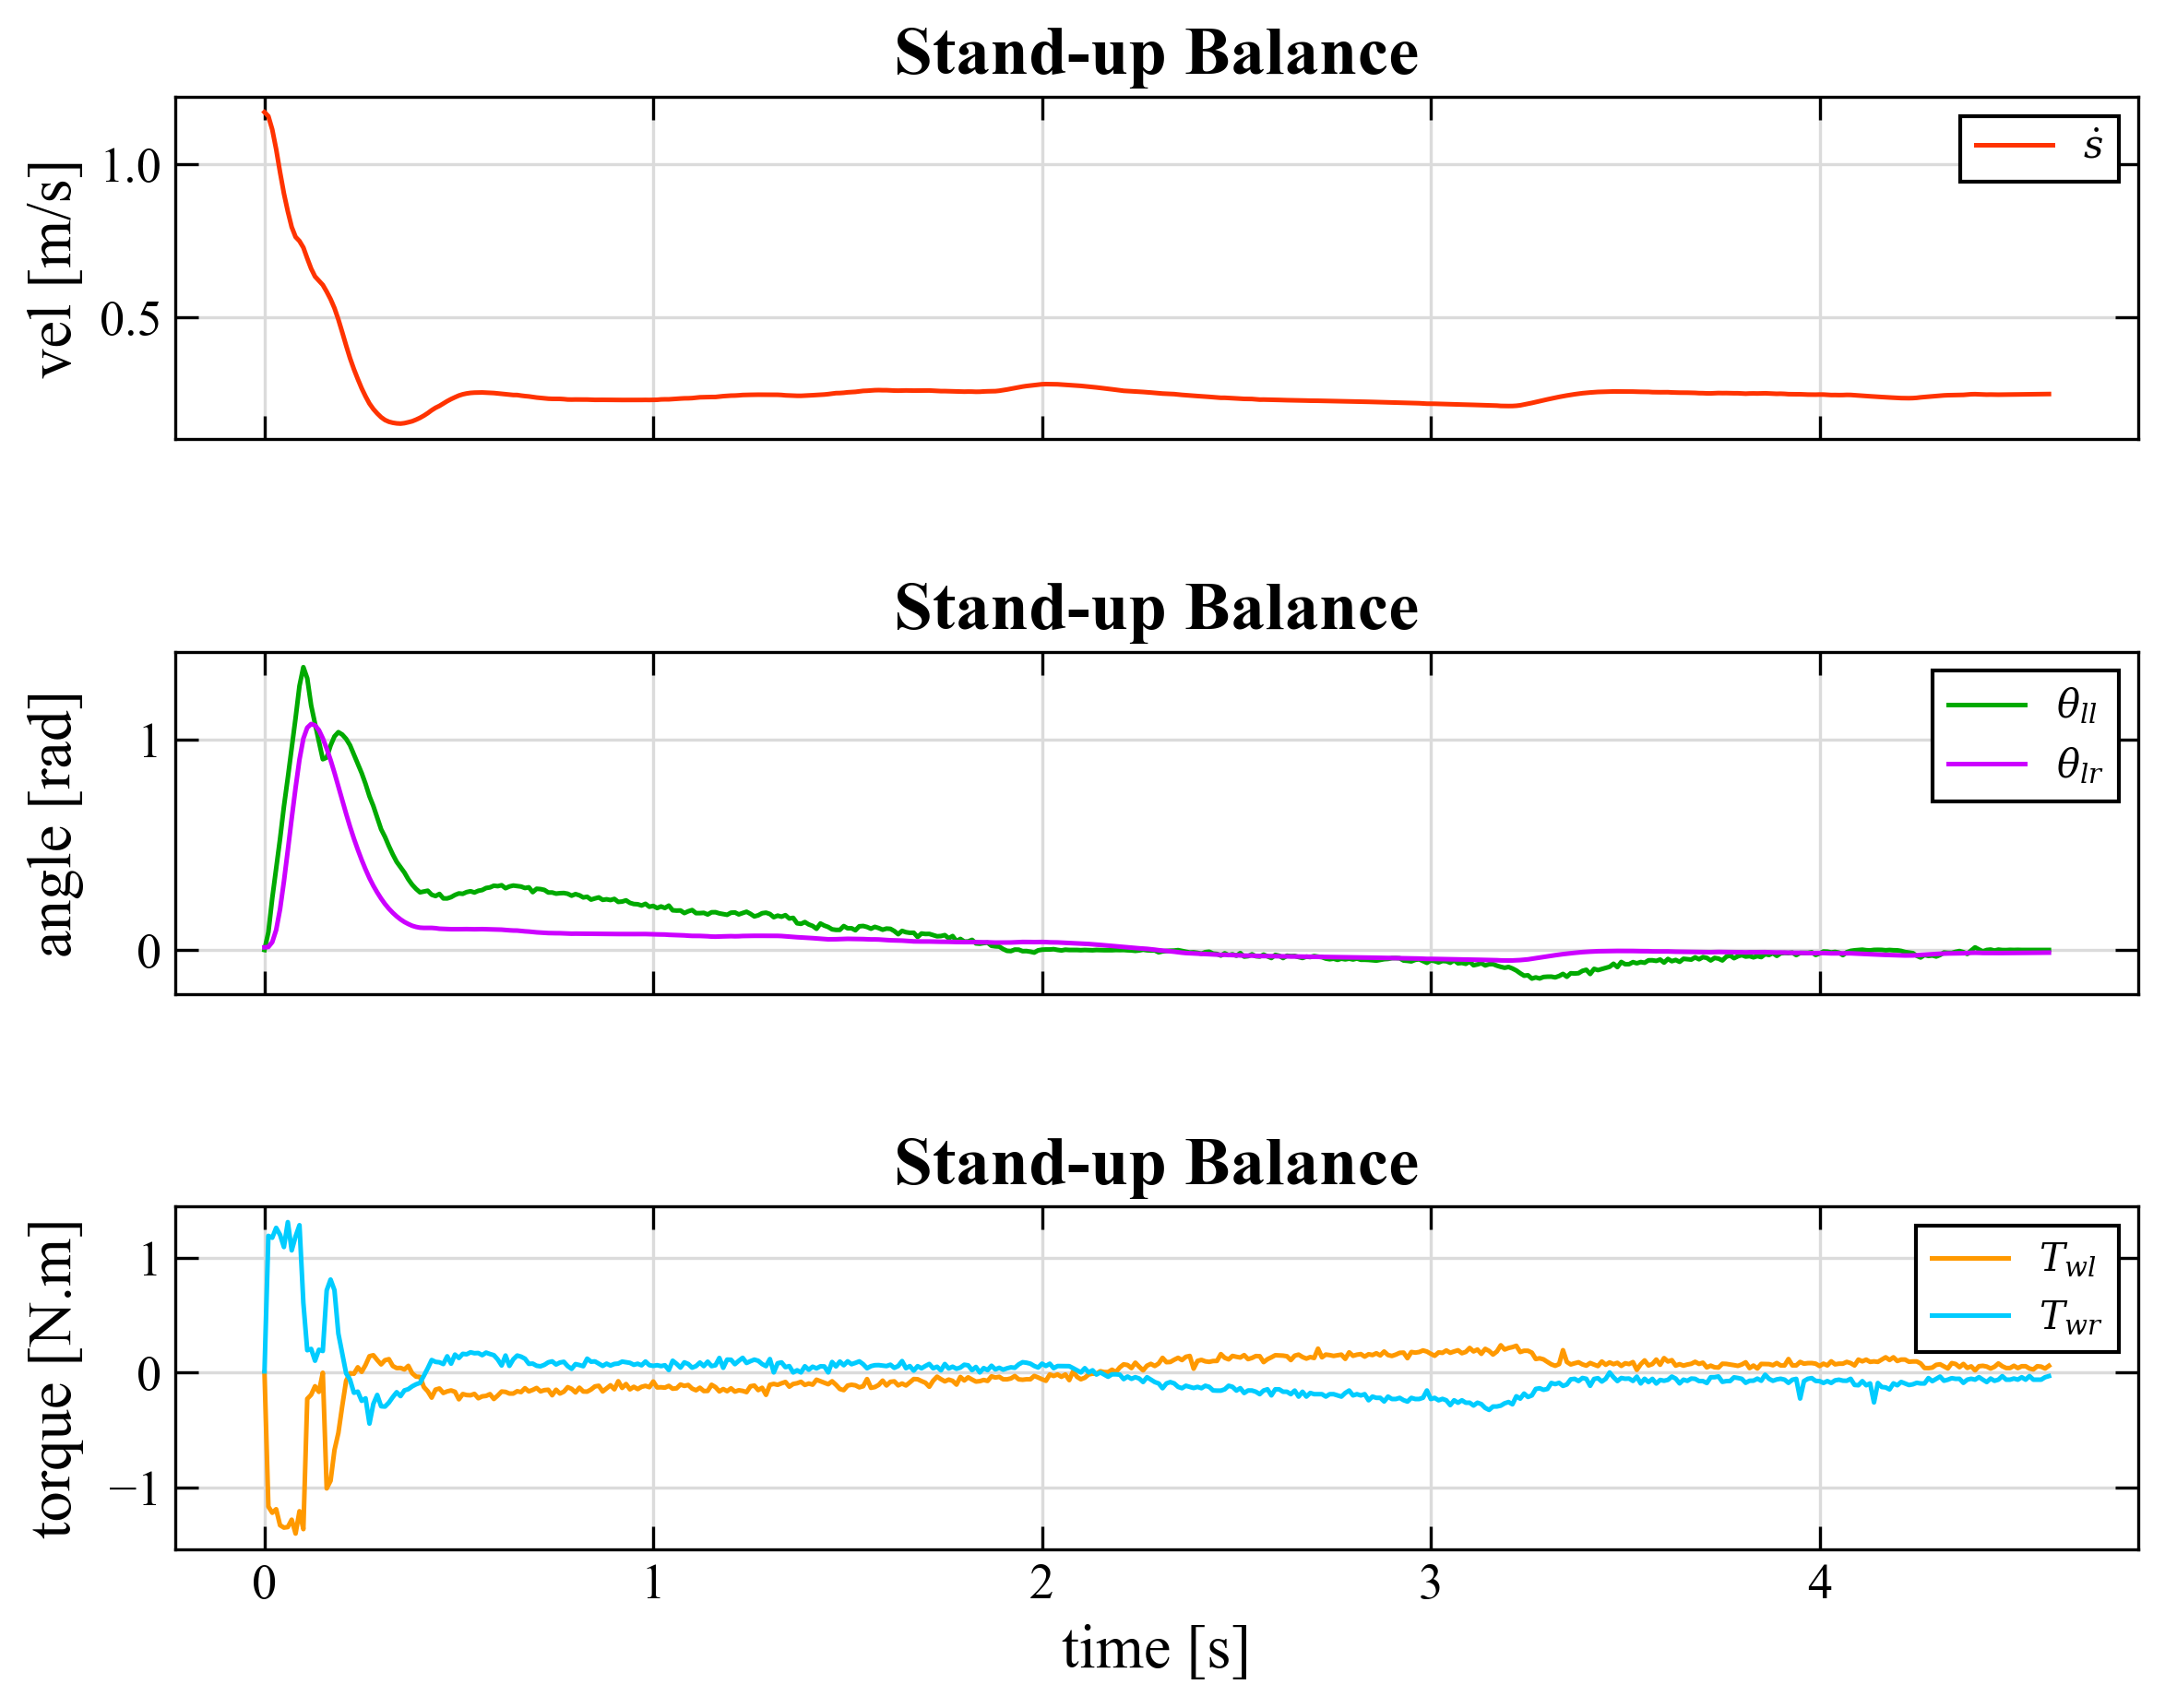
\includegraphics[width=0.6\textwidth]{figures/ch05/standup.jpg}
  \caption{原地起立并平衡过程。从上至下分别为：初始态，过渡态，平衡态}
  \label{fig:balance-experiment-scene}
\end{figure}


由\figref{fig:balance-experiment-response} 可见，起立初期机器人从支撑姿态过渡到直立姿态，前进速度和腿摆角都会出现一段较明显的瞬态变化。进入平衡阶段后，左右腿摆角回到零点附近，后续没有继续放大的低频摆动；前进速度也从起立阶段的较大变化逐渐降下来，只在零点附近小幅波动。也就是说，样机主要通过短距离前后调整来维持倒立摆平衡，并未产生明显的持续位移。

轮端力矩的变化也与这一过程一致。起立初期，两侧轮电机输出方向相反，幅值相对较大，用于快速修正机体姿态；平衡建立后，左右轮端力矩逐渐减小，并围绕零点附近波动，没有出现长时间饱和。两侧力矩曲线整体较为接近，说明样机左右传动和控制响应没有明显偏差。上述结果表明，LQR 与 VMC 在实物平台上能够配合完成原地起立和平衡保持。

\section{速度跟踪性能验证}

速度跟踪实验用于验证 LQR 控制器在速度调节和机体姿态稳定之间的协调能力。实验中，机器人先完成原地平衡，随后给定分段常值的速度参考。为降低速度指令突变对轮端摩擦和机体姿态的冲击，程序中对速度参考加入斜坡限幅。

\begin{figure}[H]
  \centering
  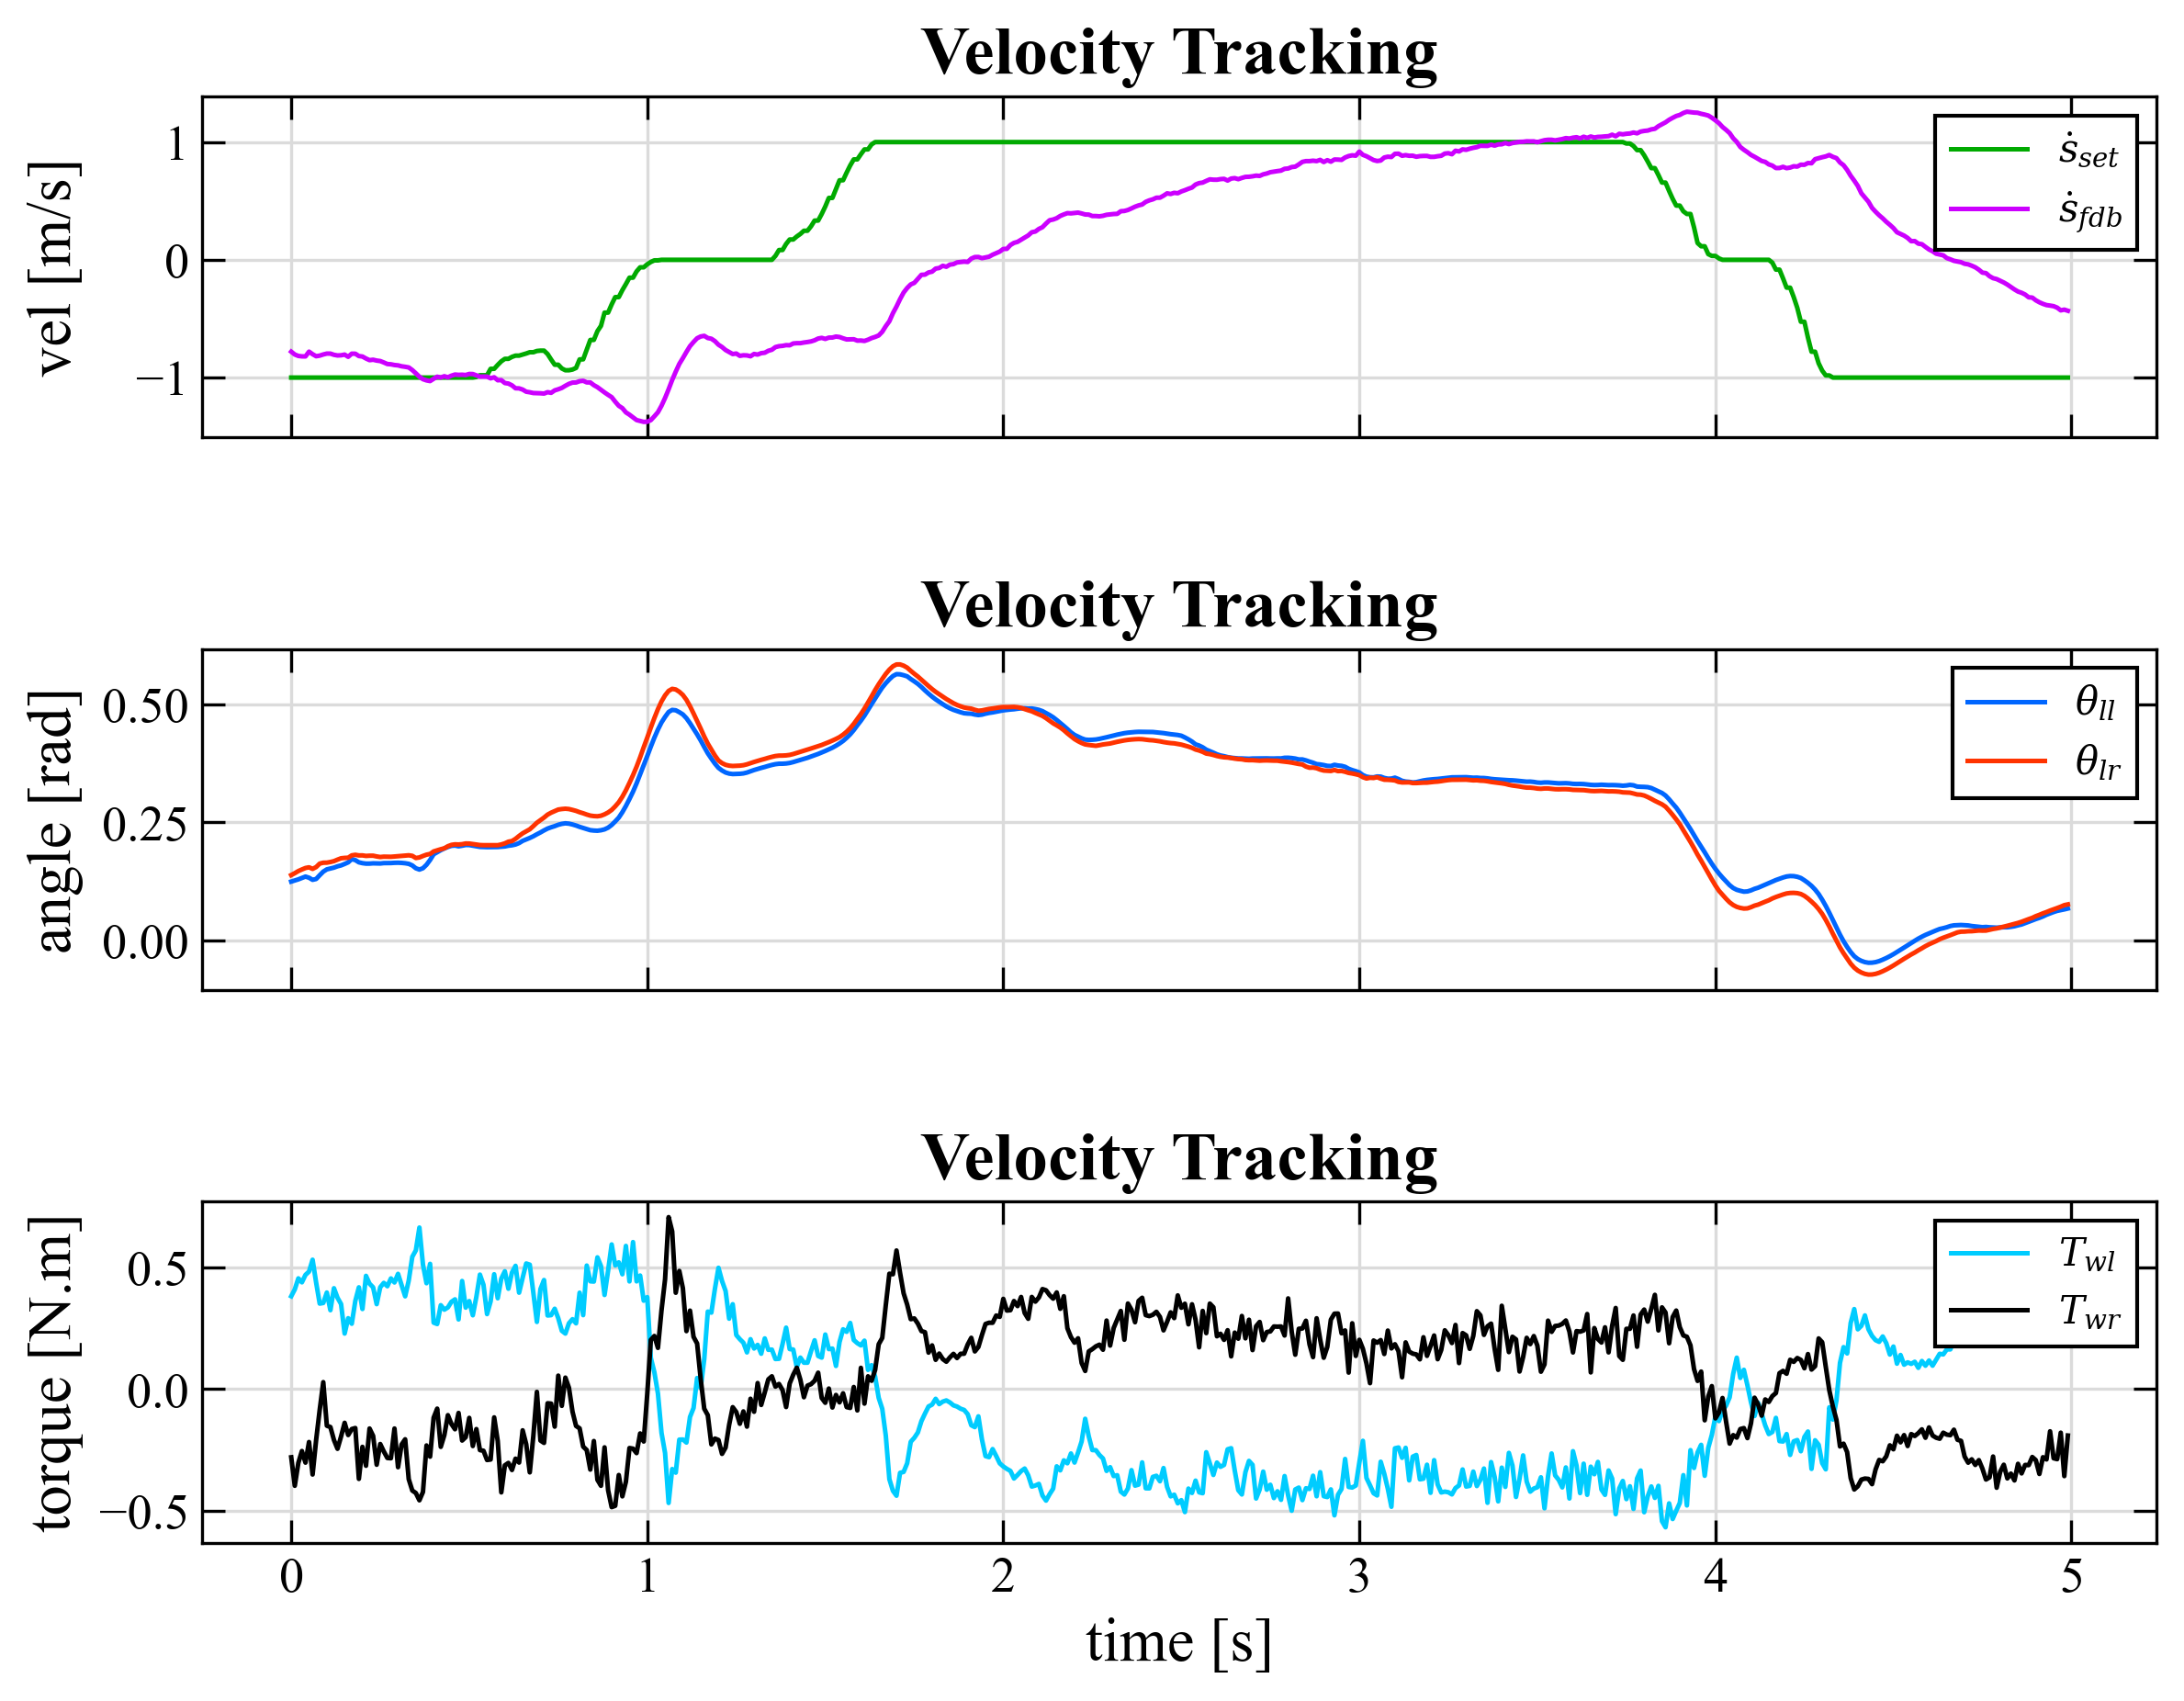
\includegraphics[width=0.9\textwidth]{figures/ch05/ds.png}
  \caption{速度跟踪实验响应曲线}
  \label{fig:velocity-experiment-response}
\end{figure}

速度跟踪实验结果如\figref{fig:velocity-experiment-response} 所示。当速度参考由负向或零附近逐渐切换至正向时，实际速度能够跟随参考速度变化，并在加速阶段呈现连续上升趋势。由于实物样机存在轮地摩擦变化、电机响应滞后和速度估计滤波延迟，实际速度相对于参考速度存在一定滞后，且在参考速度变化较快时会出现短时跟踪误差。该现象符合物理平台的实际运动特性。

\begin{figure}[H]
  \centering
  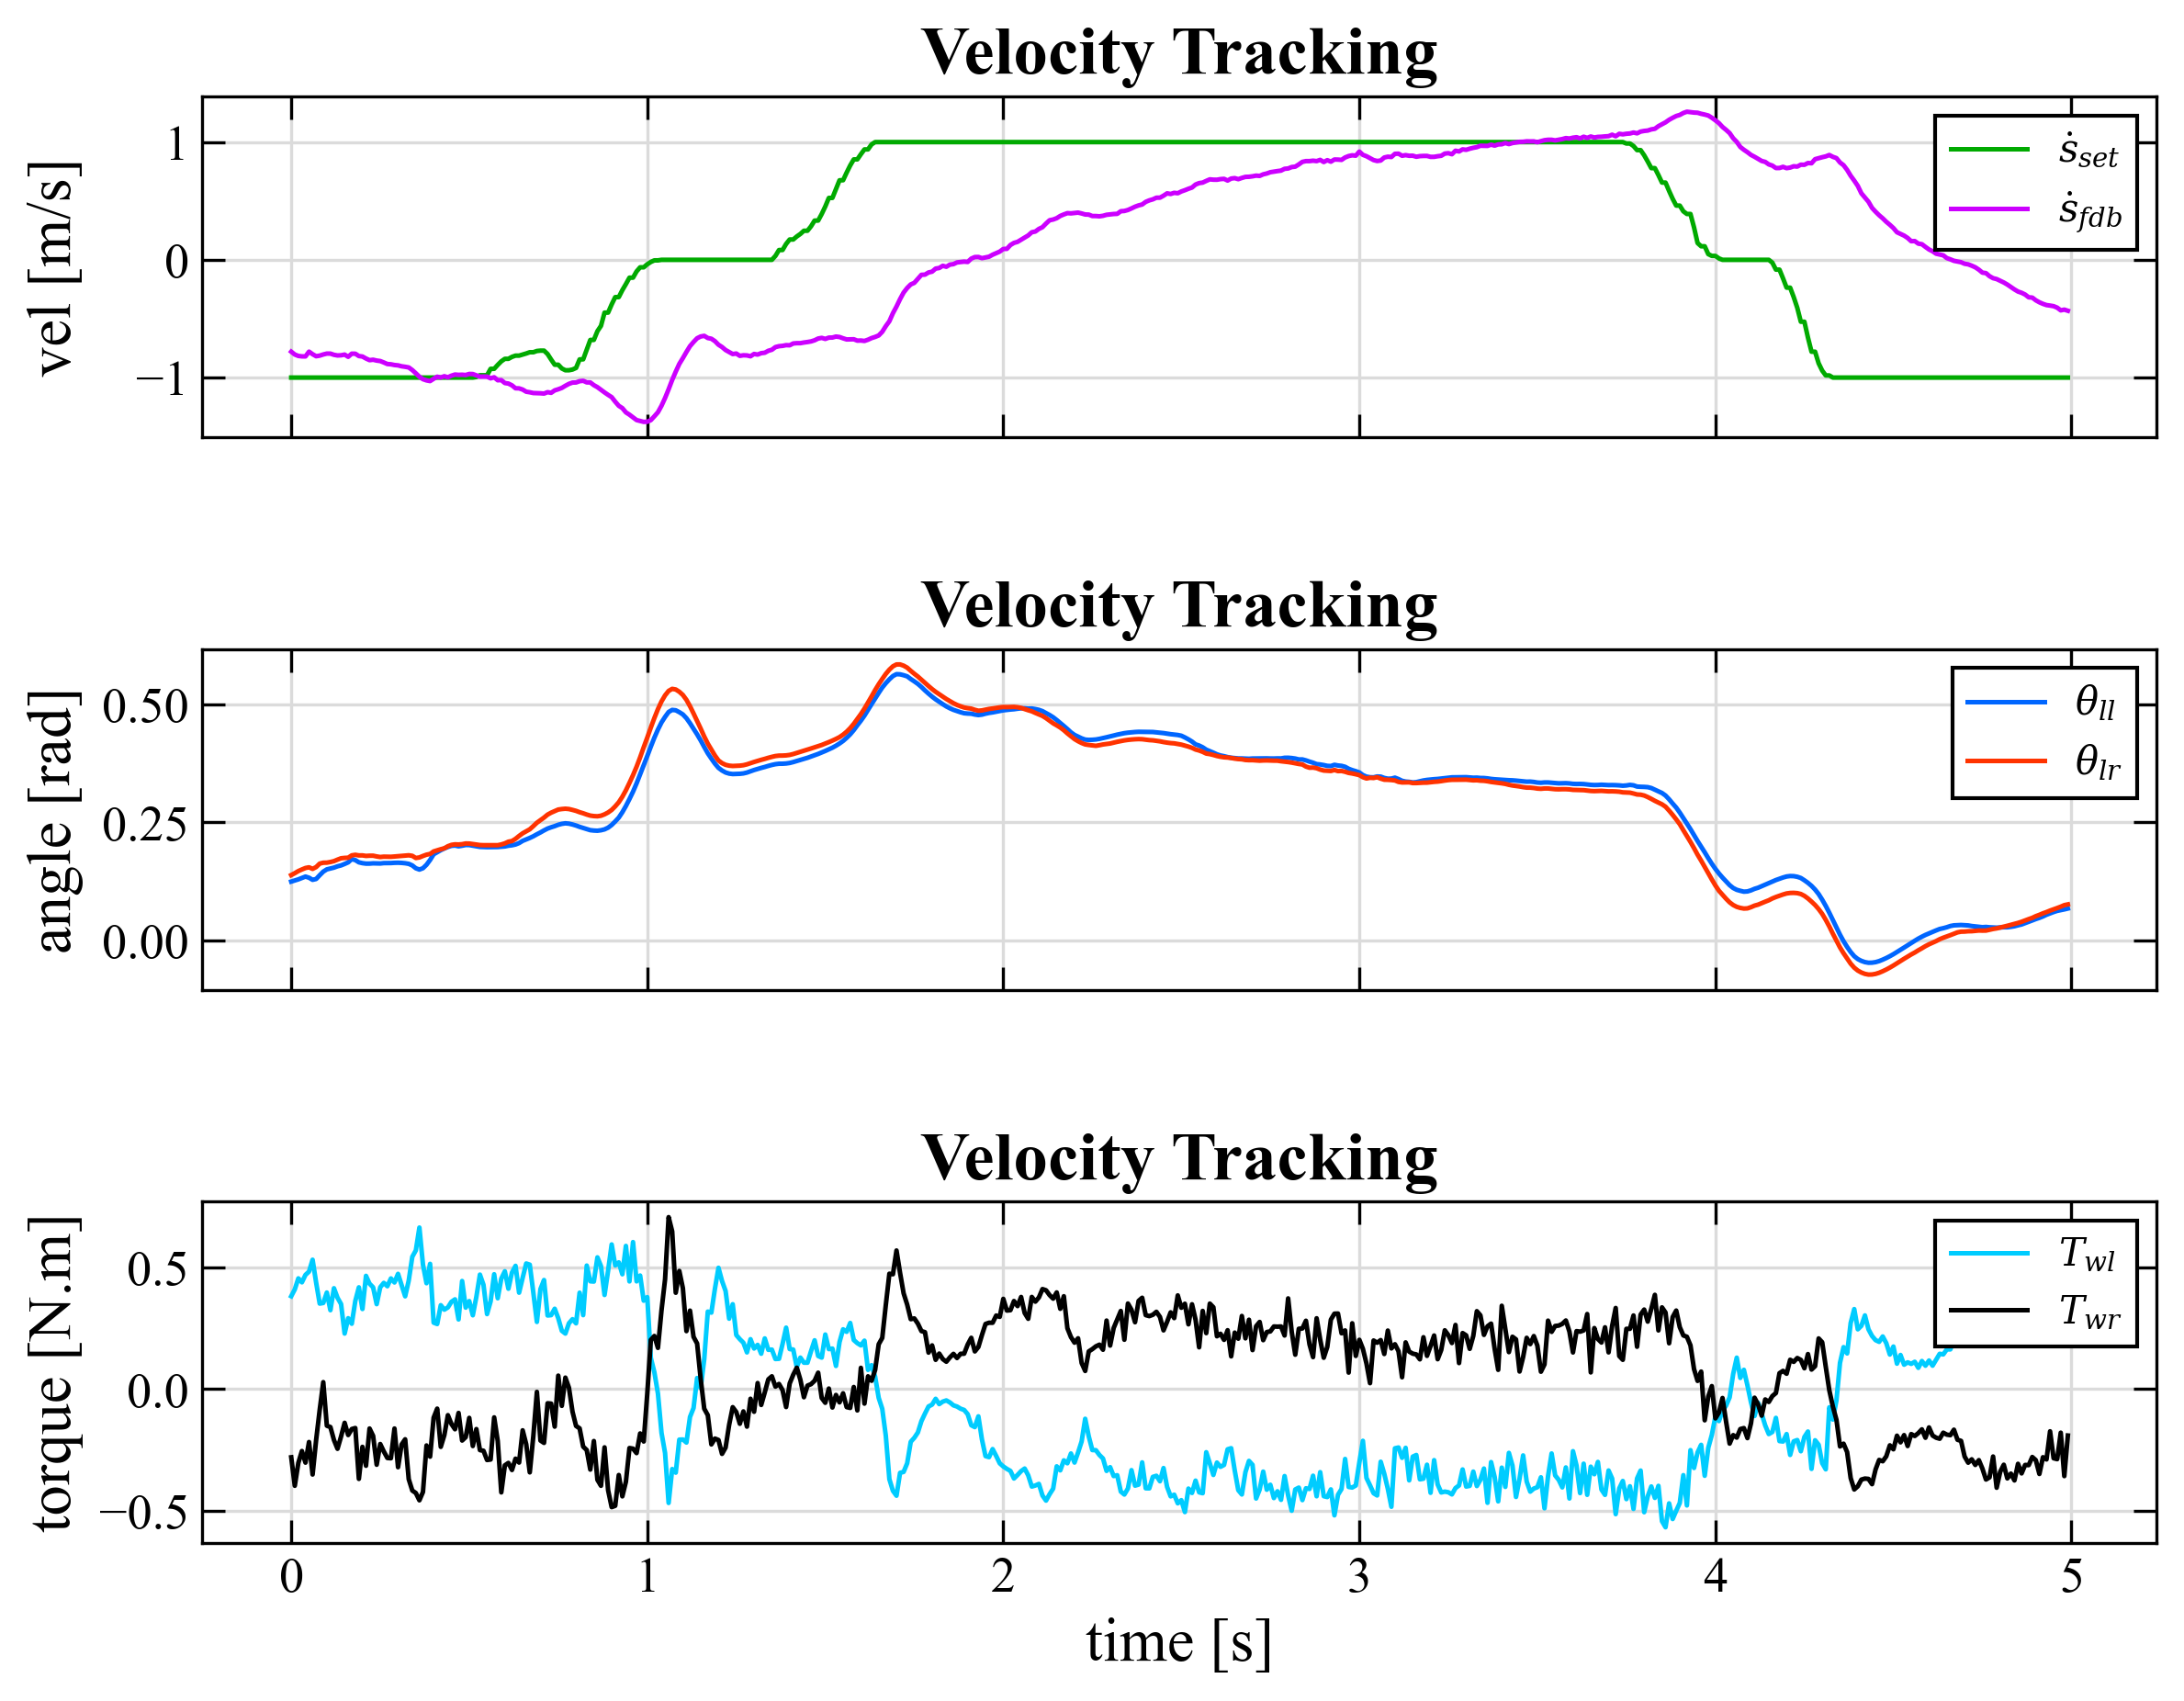
\includegraphics[width=0.5\textwidth]{figures/ch05/ds.jpg}
  \caption{速度跟踪机器人位姿表现。从上至下依次为：平衡态，加速态，匀速态}
  \label{fig:velocity-experiment-scene}
\end{figure}

速度调节期间，左右腿摆角基本同步变化，没有出现单侧腿摆明显偏离的情况。样机加减速时主要依靠机体整体前后倾斜，并配合轮端驱动力完成速度调整。当速度参考由正向切换为反向时，腿摆角会先减小，再短暂向反方向偏转，这与双轮倒立摆减速、反向时的姿态调整过程一致。轮端力矩在速度切换阶段波动较大；参考速度变化趋缓后，力矩幅值也随之回落。

\section{腿长控制验证}

腿长控制实验用于验证 VMC 腿长通道在物理样机上的高度调节和支撑能力。实验中，机器人首先保持原地平衡，随后给定左右腿公共腿长参考 $l_d$ 的周期性升降指令，并记录左右实际腿长的跟踪过程。该实验不额外改变 LQR 主控制律，腿摆方向仍由 LQR 输出控制量，因此可以较为独立地观察 VMC 腿长控制对机体高度变化的影响。

\begin{figure}[H]
  \centering
  \includegraphics[width=0.55\textwidth]{figures/ch05/leg.jpg}
  \caption{腿长控制机器人位姿表现}
  \label{fig:leg-experiment-scene}
\end{figure}

\begin{figure}[H]
  \centering
  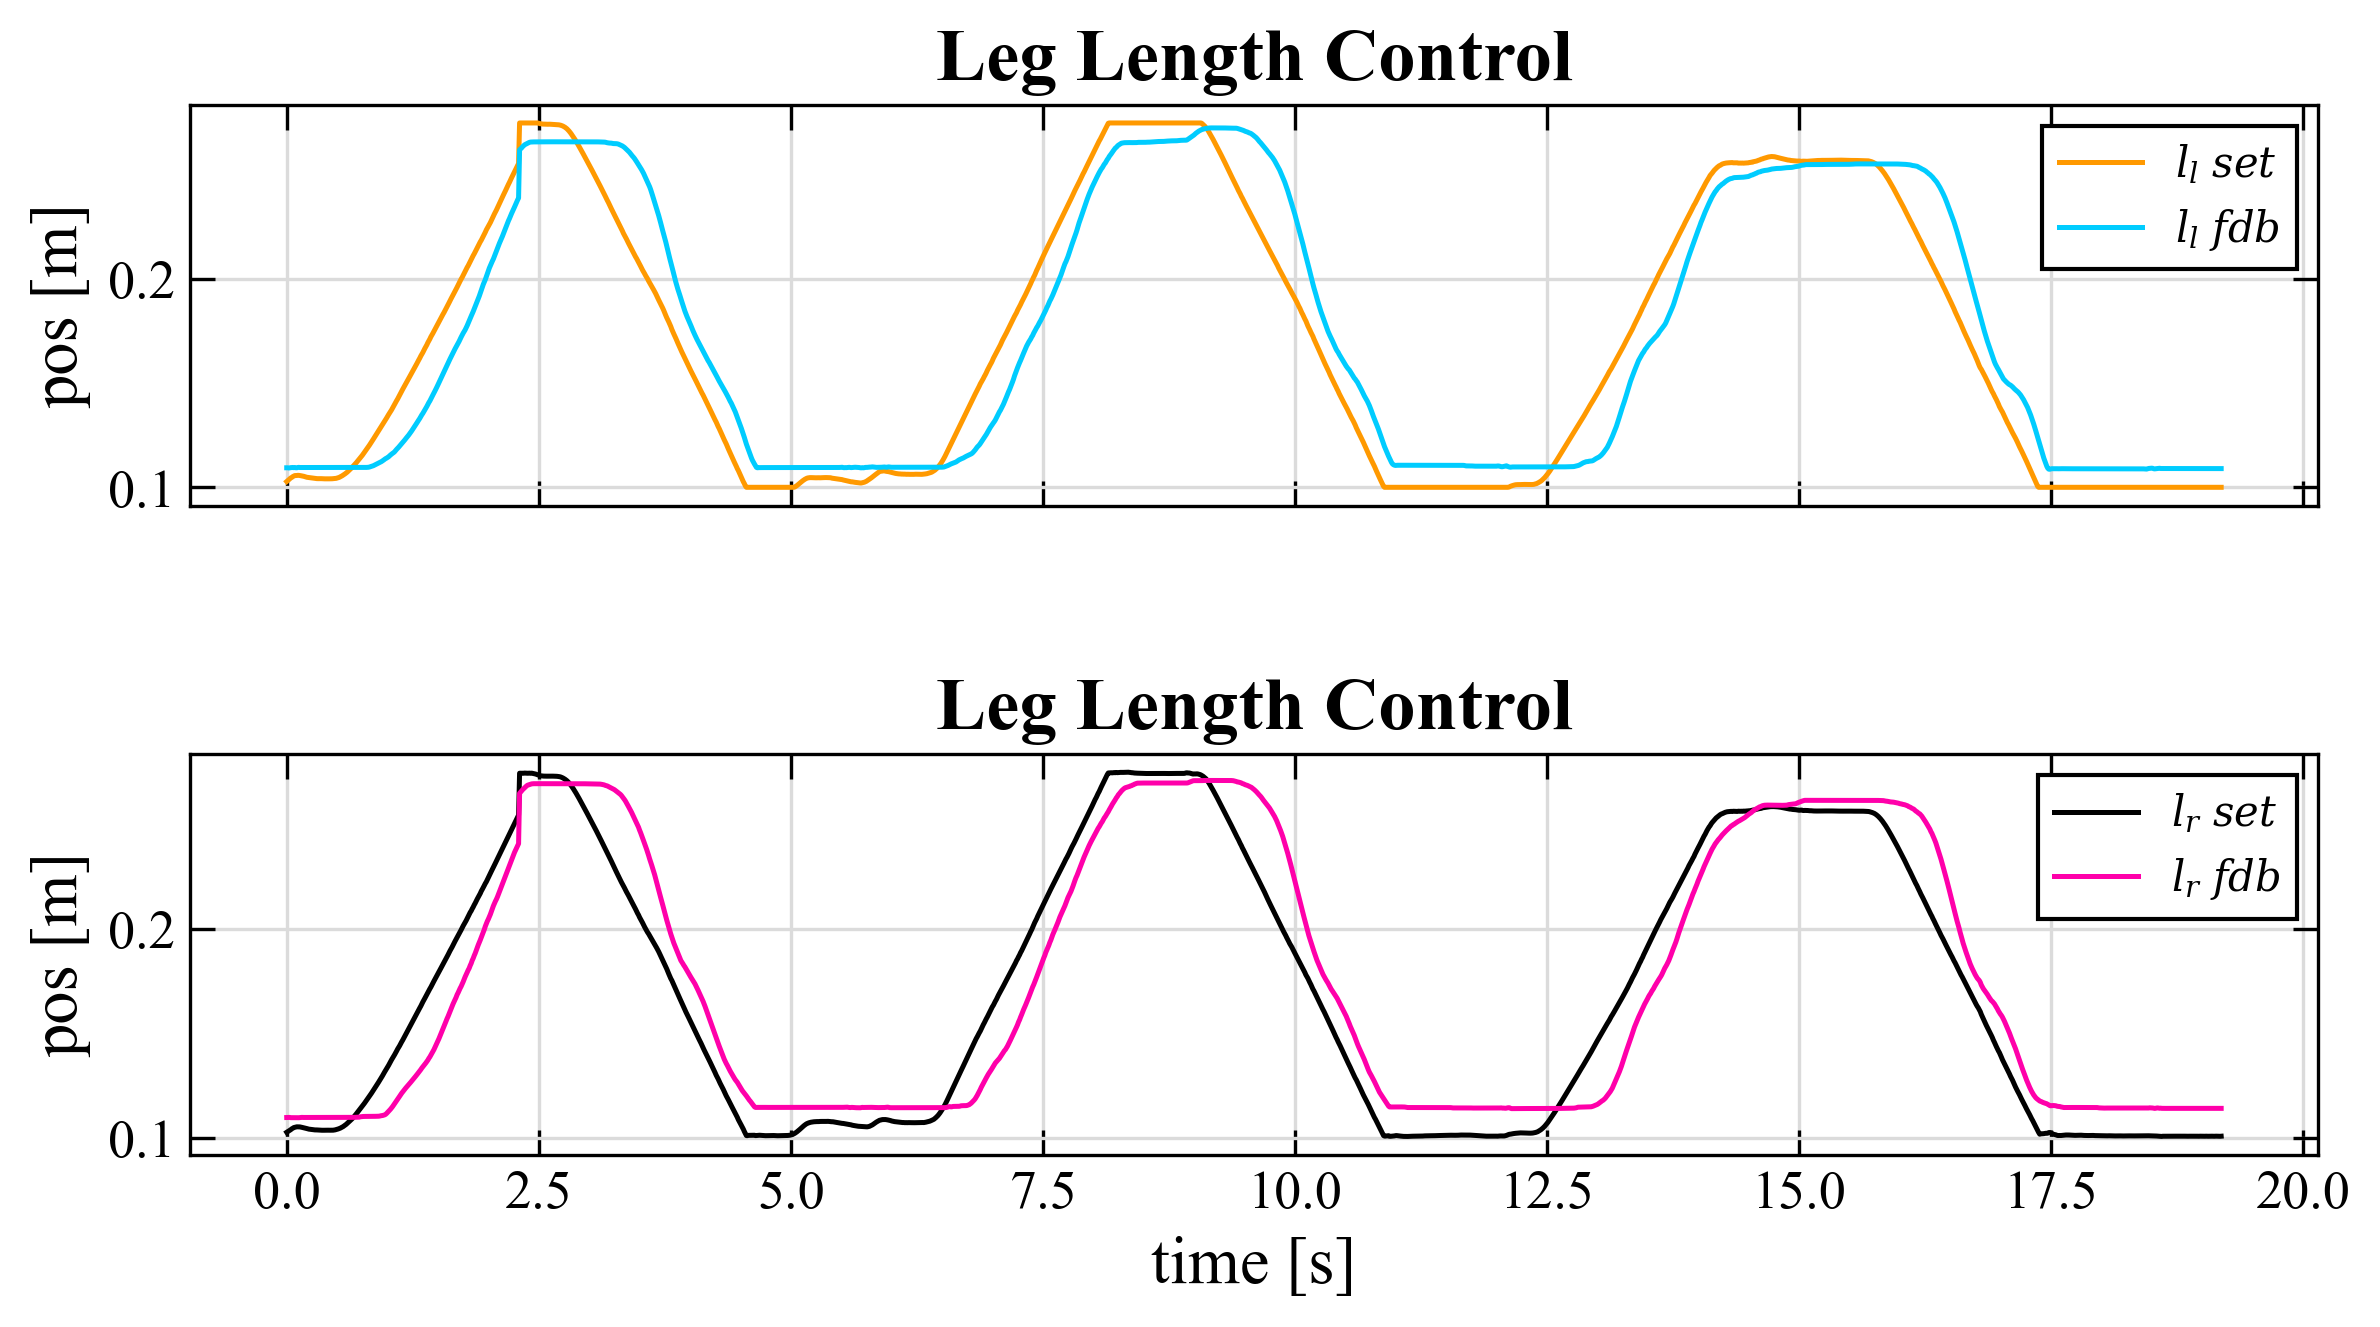
\includegraphics[width=0.8\textwidth]{figures/ch05/leg_control.png}
  \caption{腿长控制实验响应对比}
  \label{fig:leg-experiment-response}
\end{figure}

由\figref{fig:leg-experiment-response} 可见，左右腿参考长度在低位和高位之间周期性切换，实际腿长也随之完成伸长和缩短。两侧响应趋势接近，没有出现一侧明显快于另一侧或长期偏离参考值的情况，说明腿部机构装配和驱动参数整体比较一致。该结果也表明，第三章的腿部运动学解算和第四章的 VMC 腿长控制律可以在样机上闭环运行。

实际腿长相对于参考腿长仍存在一定滞后，尤其在参考值快速上升或下降时更明显。这一部分滞后主要来自电机响应、链传动间隙、腿部连杆惯量以及程序中的指令限幅。进入高位或低位保持阶段后，实际腿长能够停留在参考值附近，没有持续振荡。由此可见，当前虚拟弹簧阻尼参数没有单纯追求最快响应，而是在响应速度和稳定性之间取了较保守的设置。继续增大腿长刚度可以缩短调节时间，但会提高关节力矩峰值，也更容易激发结构振动；阻尼过大则会让腿长变化变慢。因此，实物调参时需要同时看腿长误差、关节力矩和机体姿态变化。

在腿长周期性升降的过程中，机器人仍能保持基本平衡，未出现由高度调节引起的明显俯仰失稳。这说明 VMC 腿长通道接入后没有破坏 LQR 主平衡闭环。也就是说，腿长支撑和倒立摆平衡可以通过任务空间力矩映射同时作用在腿部执行器上，实验结果与第四章的分层控制设计相符。

\section{滚转稳定性能验证}

第三章建立的主动力学模型主要描述机器人前进方向、腿摆和机体俯仰之间的耦合关系，并未将滚转角直接纳入 LQR 主控制器。实际样机在侧向扰动、转向或左右支撑高度不一致的情况下，机体会产生滚转角偏差，进而导致左右腿支撑状态不同。本节通过滚转稳定实验验证第四章提出的基于腿长差修正的侧向稳定方法。

实验中，样机在保持主平衡控制闭环的同时开启滚转稳定。滚转稳定根据测得的机体滚转角和当前腿部几何关系，计算左右腿期望腿长差，并将其叠加到左右腿长参考值中。与直接构造侧向力矩的方法相比，该补偿方式不改变 LQR-VMC 主控制框架，仅通过调整左右支撑几何关系抑制机体侧倾，因而具有实现简单、计算量小的特点。

\begin{figure}[H]
  \centering
  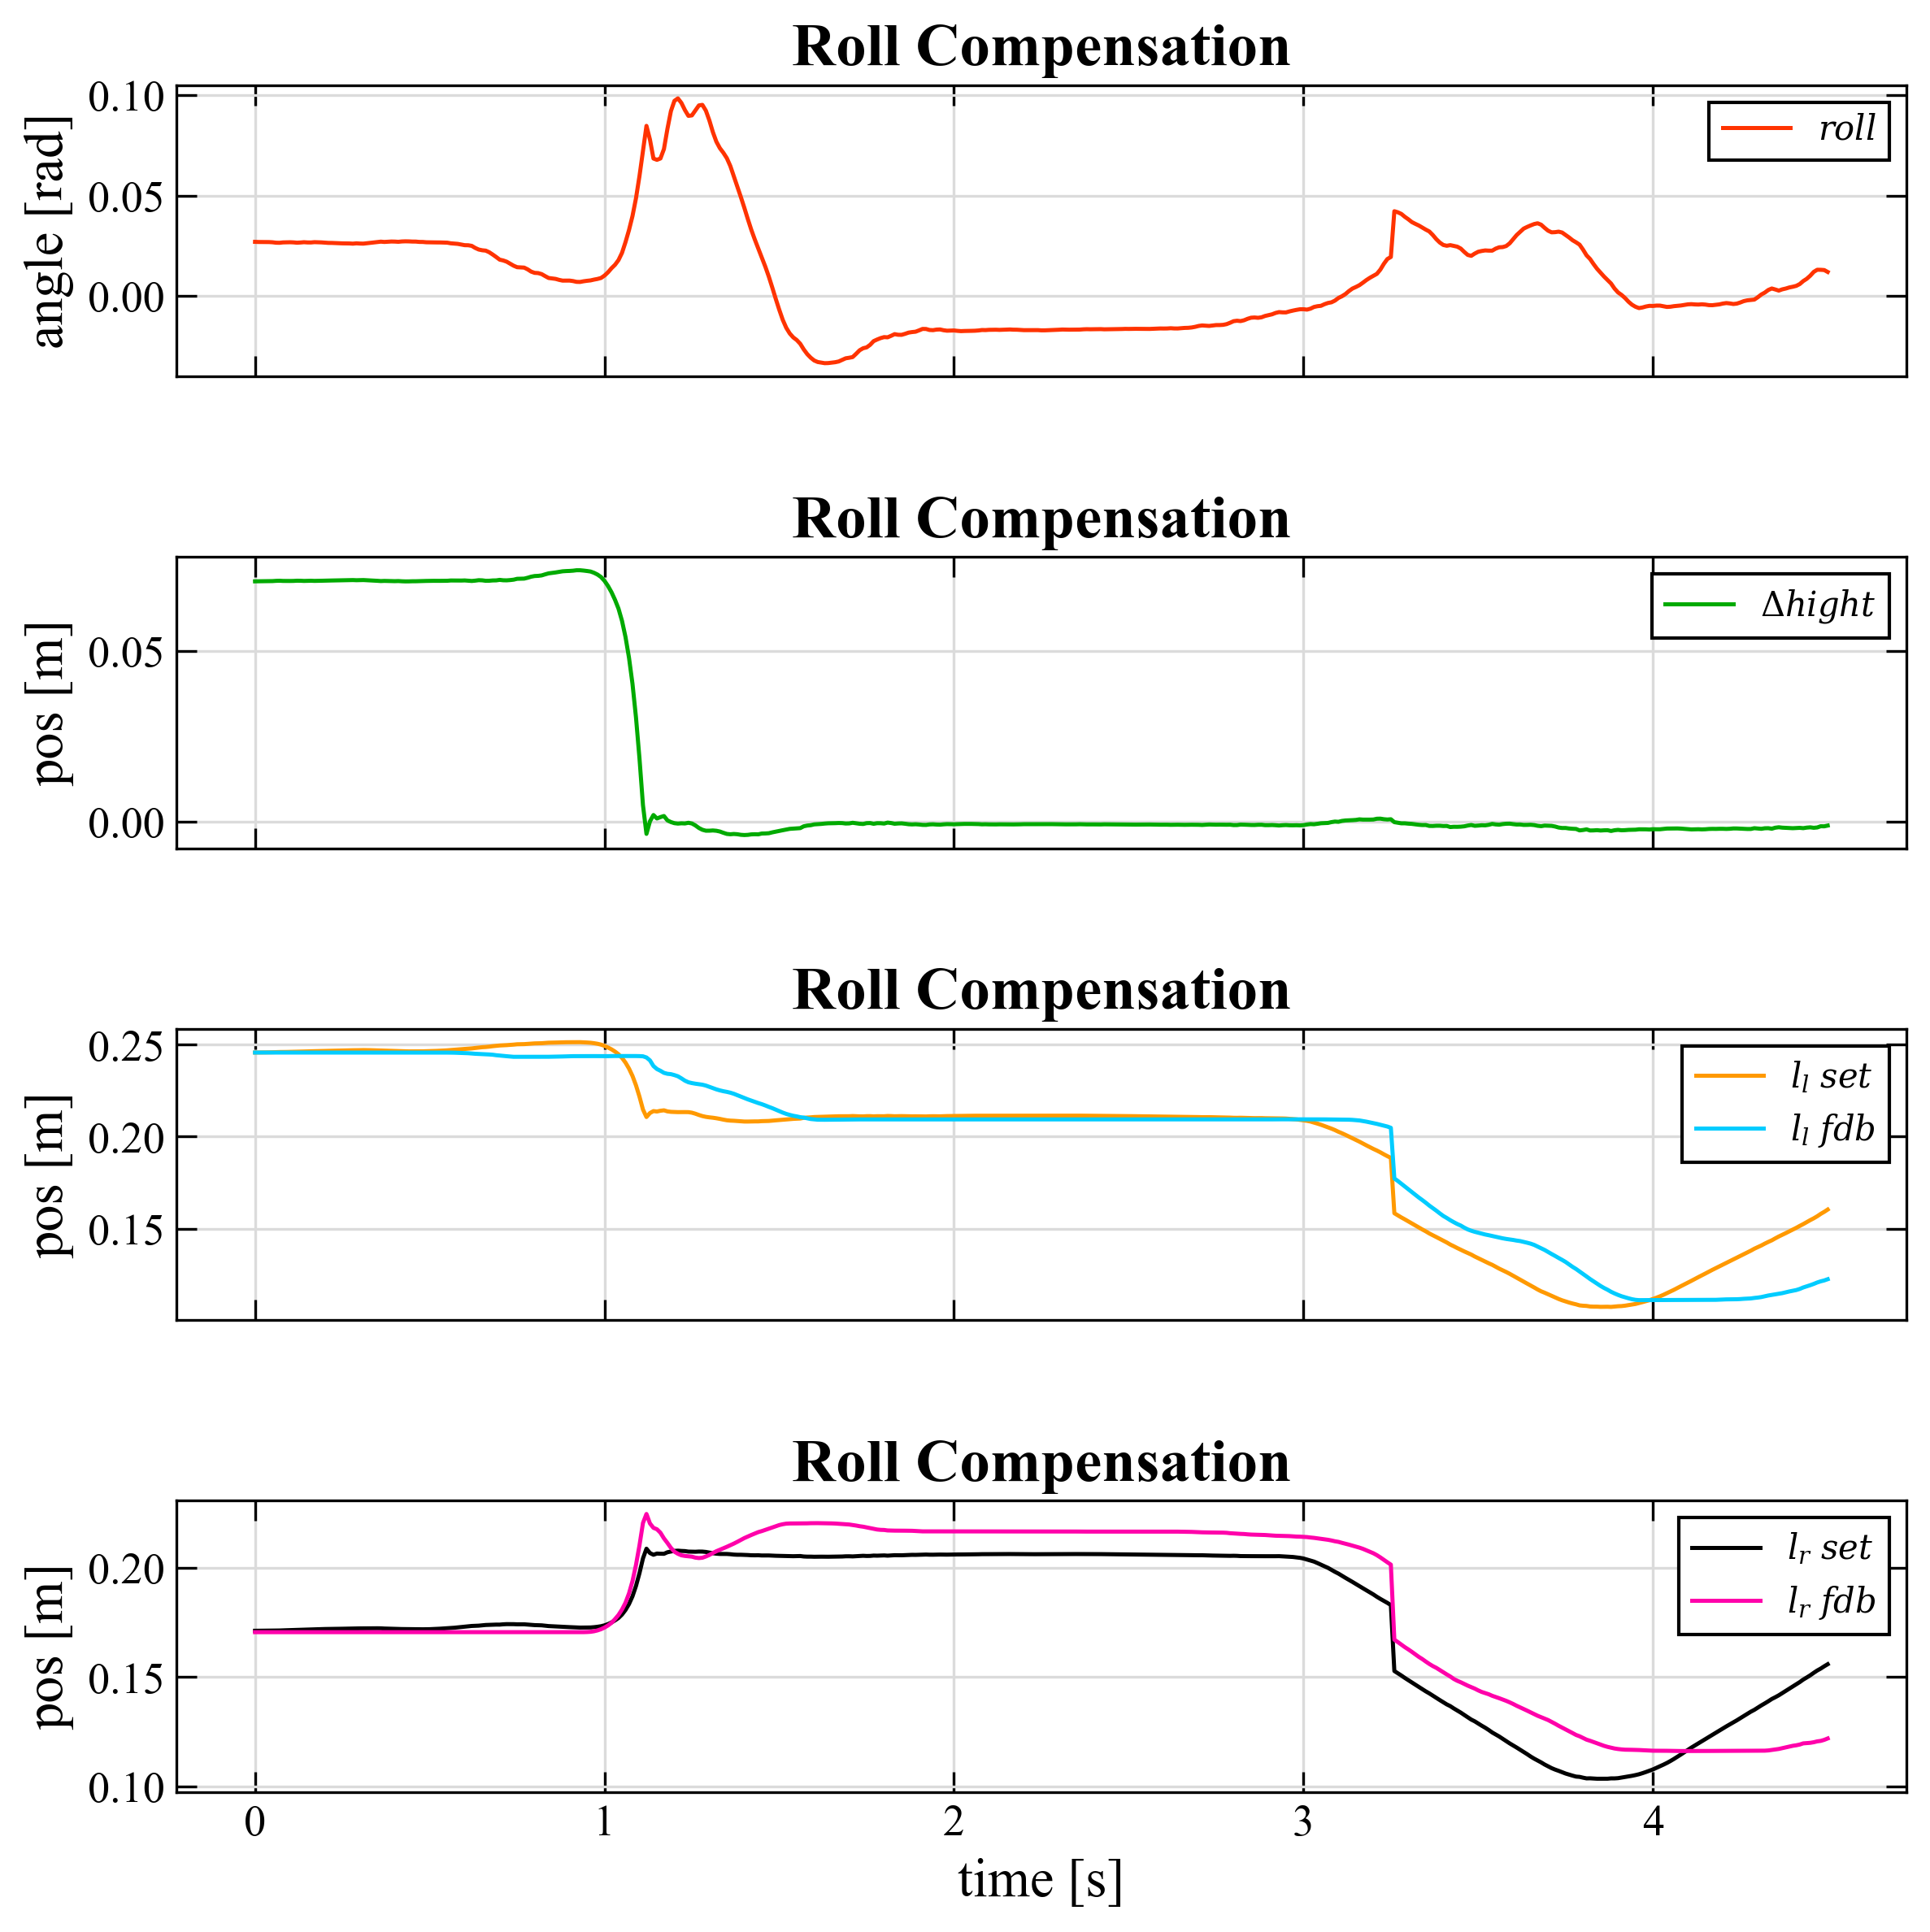
\includegraphics[width=0.7\textwidth]{figures/ch05/roll_compensation.png}
  \caption{滚转稳定前后实验响应对比}
  \label{fig:roll-experiment-response}
\end{figure}

滚转稳定实验结果如\figref{fig:roll-experiment-response} 所示。实验过程中，机体滚转角在扰动作用下出现明显偏移，随后逐渐回到零点附近。与此同时，左右腿长参考值不再保持完全相同，而是根据滚转角变化形成相反方向的修正量。该现象说明滚转稳定环节已经参与腿长通道控制，并能够通过改变左右腿支撑高度对机体侧倾进行修正。

实验结果表明，基于腿长差修正的滚转稳定能够在不改变主控制框架的前提下改善样机侧向姿态。该方法适合用于平地低速运动和轻微侧向扰动场景，但对于高速转向、强侧向冲击或复杂三维地形，仍需结合更完整的侧向动力学模型和接触力分配策略进一步优化。

\begin{figure}[H]
  \centering
  \includegraphics[width=0.6\textwidth]{figures/ch05/roll.jpg}
  \caption{滚转稳定机器人位姿表现}
  \label{fig:roll-experiment-scene}
\end{figure}

\section{本章小结}

本章在物理样机上验证了第四章设计的 LQR-VMC 分层控制器。表\ref{tab:experiment-summary} 汇总了各工况下的关键定量指标。

\begin{table}[H]
  \centering
  \caption{各工况关键实验指标汇总}
  \label{tab:experiment-summary}
  \small
  \begin{tabular}{p{2.4cm}p{2.6cm}p{2.6cm}p{2.6cm}p{2.6cm}}
    \toprule
    指标 & 原地平衡 & 速度跟踪 & 腿长控制 & 滚转稳定 \\
    \midrule
    核心验证目标 & LQR+VMC 联合起立与平衡 & 速度 + 姿态协调 & VMC 腿长通道闭环 & 滚转角补偿有效性 \\
    \hline
    姿态稳态误差 & 俯仰角波动在 $\pm 2^\circ$ 以内（RMS 约 $1.0^\circ$--$1.5^\circ$） & 加减速期间俯仰角变化 $3^\circ$--$5^\circ$，匀速段回落至 $\pm 2^\circ$ & 高度调节期间俯仰未失稳，腿长变化对平衡的耦合在可控范围内 & 滚转角 RMS 从补偿前的约 $2.5^\circ$ 降至补偿后的约 $1.5^\circ$ \\
    \hline
    跟踪/响应性能 & 起立至平衡建立约 1--2\,s & 速度跟踪延迟约 150--300\,ms，稳态误差低于 0.05\,m/s & 腿长跟踪延迟 200--400\,ms，稳态误差在 ±3\,mm 以内 & — \\
    \hline
    执行器状态 & 平衡后轮力矩未饱和，峰值约 60\%--70\% 额定值 & 加减速阶段力矩波动较大，匀速段回落 & 关节力矩峰值由腿长刚度和速度共同决定 & 腿长差修正量在 ±5\,mm 以内 \\
    \hline
    主要局限 & 链传动间隙引入微小抖动 & 轮地摩擦变化影响稳态精度 & 快速伸缩时滞后较大 & 对快速侧向扰动响应有限 \\
    \bottomrule
  \end{tabular}
\end{table}

原地平衡实验中，样机能够完成起立并保持站立，俯仰角 RMS 值约 $1.0^\circ$--$1.5^\circ$，轮端力矩未出现长期饱和。速度跟踪实验中，实际速度可以跟随参考变化，跟踪延迟在 150--300\,ms 量级，机体姿态保持稳定。腿长控制实验中，VMC 腿长通道实现了高度调节和支撑功能，稳态腿长误差在 ±3\,mm 以内。滚转稳定实验中，滚转角补偿使 RMS 滚转角从约 $2.5^\circ$ 降至约 $1.5^\circ$，验证了基于几何关系的腿长差修正对侧向稳定性的实际改善效果。

实物实验也暴露出仿真中不明显的问题：链传动间隙带来约 50--100\,ms 的腿长响应滞后，轮地接触状态变化造成速度估计的短时波动（尤其在加减速转换阶段），滚转补偿对快速侧向扰动的响应受限于传感器带宽和腿部执行器的速度上限。上述问题与样机的机械精度、传感器配置和执行器性能直接相关，后续需从结构刚度、执行器带宽、状态估计和三维稳定控制等方面继续改进。

\chapter{总结与展望}\label{chap:conclusion}

\section{总结}

本文围绕混合式双轮足机器人的结构设计、动力学建模与轻量级控制方法开展研究，完成了从机械样机设计、控制模型建立到仿真和实物实验验证的完整流程。研究工作的主要结论如下。

在机械结构设计方面，本文根据双轮足机器人平衡移动、腿长调节、越障和嵌入式实时控制需求，完成了样机总体方案设计。样机采用躯干集中承载、闭环腿部机构支撑调节、足端轮组驱动移动的结构形式，并对腿部连杆、躯干结构、髋关节轴系、链传动和轮组系统进行了设计。通过关键尺寸分析、链传动校核以及腿部关节电机和轮毂电机选型，验证了样机结构方案的可实现性，为后续控制系统搭建提供了硬件基础。

在建模与力矩映射方面，本文将复杂闭环腿部机构等效为可伸缩虚拟腿，建立了机器人平面等效运动学与动力学模型，并推导了 LQR 控制器所需的线性状态空间模型。针对实际样机采用的混合式闭环腿部结构，进一步建立了虚拟腿任务空间到关节空间的力矩映射关系。

在控制方法与实验验证方面，本文提出了 LQR-VMC 分层轻量级控制系统。LQR 用于机体平衡、速度跟踪和腿摆控制量分配，VMC 用于腿长方向支撑与高度调节，滚转稳定环节通过左右腿长差修正改善侧向姿态。MuJoCo 仿真验证了控制器在原地平衡、速度跟踪、扰动恢复和腿长调节等工况下的闭环响应。物理样机实验进一步表明，所设计的控制系统能够在真实硬件上实现起立平衡、速度调节、腿长跟踪和滚转稳定，验证了本文结构方案、建模方法和控制策略的有效性。

\section{展望}

本文仍有若干不足需要在后续研究中完善。首先，本文建立的主动力学模型以平面运动为主，对滚转方向和复杂三维接触的描述仍较简化。后续可引入三维动力学模型、接触力估计和转向状态前馈，以提高机器人在高速转向、横坡和侧向冲击工况下的稳定性。其次，实物样机仍受到链传动回差、结构弹性、执行器响应滞后和轮地接触变化的影响，后续可从机械刚度、传动精度、驱动带宽和传感器融合精度等方面继续优化。

在控制算法方面，本文采用的 LQR-VMC 方法结构清晰、计算量较小，适合当前样机的嵌入式实时实现。但随着机器人运动速度、地形复杂度和任务要求的提高，后续可进一步引入更高级的控制方法。例如，模型预测控制（MPC）能够在滚动优化过程中显式考虑动力学约束、执行器限幅和接触约束，已有轮式双足和四足机器人研究表明，MPC 可用于提升全身姿态跟踪和动态运动能力\cite{yu2023hotwheel,dicarlo2018mpc}。此外，强化学习（RL）在腿式机器人运动控制中也表现出较强的策略搜索和复杂地形适应能力，相关研究已经实现了从仿真训练到实机部署的动态运动技能学习\cite{hwangbo2019learning,miki2022perceptive,rudin2021minutes}。因此，后续可以在现有轻量级控制框架的基础上，将 MPC 用于高层轨迹和接触力规划，或将 RL 用于参数自适应、复杂地形策略生成和鲁棒控制补偿，从而提升机器人在非结构化环境中的自主运动能力。


\makereferences

\appendix
\appendixsection{机器人运动学方程完整推导}\label{app:kinematics}

本附录给出第三章中未完全展开的左右腿运动学方程。为便于与控制器状态变量对应，记左、右轮转角为 $\theta_{w,l}$、$\theta_{w,r}$，左、右虚拟腿摆角为 $\theta_{l,l}$、$\theta_{l,r}$，左、右虚拟腿长度为 $l_l$、$l_r$，轮半径为 $R_w$，半轮距为 $R_l$。

\appendixsubsection{位置方程}

\begin{gather}
  s = \frac{R_w(\theta_{w,l}+\theta_{w,r})}{2} \\
  h_b = \frac{l_l\cos\theta_{l,l}}{2}+\frac{l_r\cos\theta_{l,r}}{2} \\
  s_{l,l} = R_w\theta_{w,l}+l_{w,l}\sin\theta_{l,l} \\
  s_{l,r} = R_w\theta_{w,r}+l_{w,r}\sin\theta_{l,r} \\
  h_{l,l} = \frac{l_l\cos\theta_{l,l}}{2}+\frac{l_r\cos\theta_{l,r}}{2}-l_{b,l}\cos\theta_{l,l} \\
  h_{l,r} = \frac{l_l\cos\theta_{l,l}}{2}+\frac{l_r\cos\theta_{l,r}}{2}-l_{b,r}\cos\theta_{l,r} \\
  \phi = \frac{R_w(-\theta_{w,l}+\theta_{w,r})}{2R_l}
  -\frac{l_l\sin\theta_{l,l}}{2R_l}
  +\frac{l_r\sin\theta_{l,r}}{2R_l} \\
  s_b = \frac{R_w(\theta_{w,l}+\theta_{w,r})}{2}
  +\frac{l_l\sin\theta_{l,l}}{2}
  +\frac{l_r\sin\theta_{l,r}}{2}
\end{gather}

\appendixsubsection{速度与加速度方程}

\begin{gather}
  \dot{s} = \frac{R_w\dot{\theta}_{w,l}}{2}+\frac{R_w\dot{\theta}_{w,r}}{2} \\
  \ddot{s} = \frac{R_w\ddot{\theta}_{w,l}}{2}+\frac{R_w\ddot{\theta}_{w,r}}{2} \\
  \dot{\phi} =
  -\frac{R_w\dot{\theta}_{w,l}}{2R_l}
  +\frac{R_w\dot{\theta}_{w,r}}{2R_l}
  -\frac{\dot{\theta}_{l,l}l_l\cos\theta_{l,l}}{2R_l}
  +\frac{\dot{\theta}_{l,r}l_r\cos\theta_{l,r}}{2R_l} \\
  \ddot{\phi} =
  -\frac{R_w\ddot{\theta}_{w,l}}{2R_l}
  +\frac{R_w\ddot{\theta}_{w,r}}{2R_l}
  -\frac{\ddot{\theta}_{l,l}l_l\cos\theta_{l,l}}{2R_l}
  +\frac{\ddot{\theta}_{l,r}l_r\cos\theta_{l,r}}{2R_l}
  +\frac{\dot{\theta}_{l,l}^2l_l\sin\theta_{l,l}}{2R_l}
  -\frac{\dot{\theta}_{l,r}^2l_r\sin\theta_{l,r}}{2R_l} \\
  \dot{s}_b =
  \frac{R_w\dot{\theta}_{w,l}}{2}
  +\frac{R_w\dot{\theta}_{w,r}}{2}
  +\frac{\dot{\theta}_{l,l}l_l\cos\theta_{l,l}}{2}
  +\frac{\dot{\theta}_{l,r}l_r\cos\theta_{l,r}}{2} \\
  \ddot{s}_b =
  \frac{R_w\ddot{\theta}_{w,l}}{2}
  +\frac{R_w\ddot{\theta}_{w,r}}{2}
  +\frac{\ddot{\theta}_{l,l}l_l\cos\theta_{l,l}}{2}
  +\frac{\ddot{\theta}_{l,r}l_r\cos\theta_{l,r}}{2}
  -\frac{\dot{\theta}_{l,l}^2l_l\sin\theta_{l,l}}{2}
  -\frac{\dot{\theta}_{l,r}^2l_r\sin\theta_{l,r}}{2} \\
  \dot{h}_b =
  -\frac{\dot{\theta}_{l,l}l_l\sin\theta_{l,l}}{2}
  -\frac{\dot{\theta}_{l,r}l_r\sin\theta_{l,r}}{2} \\
  \ddot{h}_b =
  -\frac{\ddot{\theta}_{l,l}l_l\sin\theta_{l,l}}{2}
  -\frac{\ddot{\theta}_{l,r}l_r\sin\theta_{l,r}}{2}
  -\frac{\dot{\theta}_{l,l}^2l_l\cos\theta_{l,l}}{2}
  -\frac{\dot{\theta}_{l,r}^2l_r\cos\theta_{l,r}}{2}
\end{gather}

\begin{gather}
  \dot{s}_{l,l} = R_w\dot{\theta}_{w,l}+\dot{\theta}_{l,l}l_{w,l}\cos\theta_{l,l} \\
  \dot{s}_{l,r} = R_w\dot{\theta}_{w,r}+\dot{\theta}_{l,r}l_{w,r}\cos\theta_{l,r} \\
  \ddot{s}_{l,l} = R_w\ddot{\theta}_{w,l}
  +\ddot{\theta}_{l,l}l_{w,l}\cos\theta_{l,l}
  -\dot{\theta}_{l,l}^2l_{w,l}\sin\theta_{l,l} \\
  \ddot{s}_{l,r} = R_w\ddot{\theta}_{w,r}
  +\ddot{\theta}_{l,r}l_{w,r}\cos\theta_{l,r}
  -\dot{\theta}_{l,r}^2l_{w,r}\sin\theta_{l,r}
\end{gather}

\begin{gather}
  \dot{h}_{l,l} =
  \dot{\theta}_{l,l}\left(-\frac{l_l\sin\theta_{l,l}}{2}+l_{b,l}\sin\theta_{l,l}\right)
  -\frac{\dot{\theta}_{l,r}l_r\sin\theta_{l,r}}{2} \\
  \dot{h}_{l,r} =
  -\frac{\dot{\theta}_{l,l}l_l\sin\theta_{l,l}}{2}
  +\dot{\theta}_{l,r}\left(-\frac{l_r\sin\theta_{l,r}}{2}+l_{b,r}\sin\theta_{l,r}\right)
\end{gather}

\begin{equation}
\begin{aligned}
  \ddot{h}_{l,l} &=
  \ddot{\theta}_{l,l}\left(-\frac{l_l\sin\theta_{l,l}}{2}+l_{b,l}\sin\theta_{l,l}\right)
  -\frac{\ddot{\theta}_{l,r}l_r\sin\theta_{l,r}}{2} \\
  &\quad
  +\dot{\theta}_{l,l}^2\left(-\frac{l_l\cos\theta_{l,l}}{2}+l_{b,l}\cos\theta_{l,l}\right)
  -\frac{\dot{\theta}_{l,r}^2l_r\cos\theta_{l,r}}{2}
\end{aligned}
\end{equation}

\begin{equation}
\begin{aligned}
  \ddot{h}_{l,r} &=
  -\frac{\ddot{\theta}_{l,l}l_l\sin\theta_{l,l}}{2}
  +\ddot{\theta}_{l,r}\left(-\frac{l_r\sin\theta_{l,r}}{2}+l_{b,r}\sin\theta_{l,r}\right) \\
  &\quad
  -\frac{\dot{\theta}_{l,l}^2l_l\cos\theta_{l,l}}{2}
  +\dot{\theta}_{l,r}^2\left(-\frac{l_r\cos\theta_{l,r}}{2}+l_{b,r}\cos\theta_{l,r}\right)
\end{aligned}
\end{equation}

\appendixsection{机器人动力学方程完整推导}\label{app:dynamics}

本附录给出第三章线性状态空间模型所依据的原始动力学方程、线性化方程组和矩阵形式。式中 $f_l$、$f_r$ 为左右轮地面切向作用力，$F_{ws}$、$F_{wh}$ 为轮端与腿部之间的水平和竖直约束力，$F_{bs}$、$F_{bh}$ 为腿部与机体之间的水平和竖直约束力。

\appendixsubsection{原始动力学方程}

\begin{gather}
  R_w\ddot{\theta}_{w,l}m_w = -F_{ws,l}+f_l \\
  R_w\ddot{\theta}_{w,r}m_w = -F_{ws,r}+f_r \\
  I_w\ddot{\theta}_{w,l} = -R_wf_l+T_{lw,l} \\
  I_w\ddot{\theta}_{w,r} = -R_wf_r+T_{lw,r} \\
  m_l(R_w\ddot{\theta}_{w,l}+\ddot{\theta}_{l,l}l_{w,l}) = -F_{bs,l}+F_{ws,l} \\
  m_l(R_w\ddot{\theta}_{w,r}+\ddot{\theta}_{l,r}l_{w,r}) = -F_{bs,r}+F_{ws,r} \\
  0 = -F_{bh,l}+F_{wh,l}-gm_l \\
  0 = -F_{bh,r}+F_{wh,r}-gm_l
\end{gather}

\begin{equation}
\begin{aligned}
  I_l\ddot{\theta}_{l,l} &=
  -F_{bs,l}l_{b,l}-F_{ws,l}l_{w,l}+T_{bl,l}-T_{lw,l} \\
  &\quad
  +\theta_{l,l}(F_{bh,l}l_{b,l}+F_{wh,l}l_{w,l})
\end{aligned}
\end{equation}

\begin{equation}
\begin{aligned}
  I_l\ddot{\theta}_{l,r} &=
  -F_{bs,r}l_{b,r}-F_{ws,r}l_{w,r}+T_{bl,r}-T_{lw,r} \\
  &\quad
  +\theta_{l,r}(F_{bh,r}l_{b,r}+F_{wh,r}l_{w,r})
\end{aligned}
\end{equation}

\begin{equation}
  m_b\left(\frac{R_w(\ddot{\theta}_{w,l}+\ddot{\theta}_{w,r})}{2}
  +\frac{\ddot{\theta}_{l,l}l_l}{2}
  +\frac{\ddot{\theta}_{l,r}l_r}{2}\right)
  = F_{bs,l}+F_{bs,r}
\end{equation}

\begin{gather}
  0 = F_{bh,l}+F_{bh,r}-gm_b
\end{gather}

\begin{equation}
\begin{aligned}
  I_b\ddot{\theta}_b &=
  -T_{bl,l}-T_{bl,r} \\
  &\quad
  +\theta_b l_c(F_{bh,l}+F_{bh,r})
  -l_c(F_{bs,l}+F_{bs,r})
\end{aligned}
\end{equation}

\begin{gather}
  I_z\ddot{\phi} = R_l(-f_l+f_r) \\
  F_{wh,l} = F_{wh,r}
\end{gather}

\appendixsubsection{线性化后的动力学方程组}

在直立平衡点附近作小角度线性化，并对约束力进行消元，可得以下五个独立方程：

\begin{align}
  &-T_{bl,l}
  +T_{lw,l}\left(1+\frac{l_{b,l}}{R_w}+\frac{l_{w,l}}{R_w}\right)
  +\ddot{\theta}_{l,l}(I_l-l_{b,l}l_{w,l}m_l) \notag\\
  &\quad
  +\ddot{\theta}_{w,l}\left(
  -\frac{I_wl_{b,l}}{R_w}
  -\frac{I_wl_{w,l}}{R_w}
  -R_wl_{b,l}m_l
  -R_wl_{b,l}m_w
  -R_wl_{w,l}m_w\right) \notag\\
  &\quad
  +\theta_{l,l}\left(
  -\frac{gl_{b,l}m_b}{2}
  -\frac{gl_{w,l}m_b}{2}
  -gl_{w,l}m_l\right)=0 \\
  &-T_{bl,r}
  +T_{lw,r}\left(1+\frac{l_{b,r}}{R_w}+\frac{l_{w,r}}{R_w}\right)
  +\ddot{\theta}_{l,r}(I_l-l_{b,r}l_{w,r}m_l) \notag\\
  &\quad
  +\ddot{\theta}_{w,r}\left(
  -\frac{I_wl_{b,r}}{R_w}
  -\frac{I_wl_{w,r}}{R_w}
  -R_wl_{b,r}m_l
  -R_wl_{b,r}m_w
  -R_wl_{w,r}m_w\right) \notag\\
  &\quad
  +\theta_{l,r}\left(
  -\frac{gl_{b,r}m_b}{2}
  -\frac{gl_{w,r}m_b}{2}
  -gl_{w,r}m_l\right)=0 \\
  &\ddot{\theta}_{l,l}\left(\frac{l_lm_b}{2}+l_{w,l}m_l\right)
  +\ddot{\theta}_{l,r}\left(\frac{l_rm_b}{2}+l_{w,r}m_l\right) \notag\\
  &\quad
  +\ddot{\theta}_{w,l}\left(\frac{I_w}{R_w}+\frac{R_wm_b}{2}+R_wm_l+R_wm_w\right)
  +\ddot{\theta}_{w,r}\left(\frac{I_w}{R_w}+\frac{R_wm_b}{2}+R_wm_l+R_wm_w\right) \notag\\
  &\quad
  -\frac{T_{lw,l}}{R_w}-\frac{T_{lw,r}}{R_w}=0 \\
  &I_b\ddot{\theta}_b+T_{bl,l}+T_{bl,r}
  -\ddot{\theta}_{l,l}l_cl_{w,l}m_l
  -\ddot{\theta}_{l,r}l_cl_{w,r}m_l \notag\\
  &\quad
  +\ddot{\theta}_{w,l}\left(-\frac{I_wl_c}{R_w}-R_wl_cm_l-R_wl_cm_w\right)
  +\ddot{\theta}_{w,r}\left(-\frac{I_wl_c}{R_w}-R_wl_cm_l-R_wl_cm_w\right) \notag\\
  &\quad
  -\theta_bgl_cm_b+\frac{T_{lw,l}l_c}{R_w}+\frac{T_{lw,r}l_c}{R_w}=0 \\
  &-\frac{I_z\ddot{\theta}_{l,l}l_l}{2R_l}
  +\frac{I_z\ddot{\theta}_{l,r}l_r}{2R_l}
  +\frac{R_lT_{lw,l}}{R_w}
  -\frac{R_lT_{lw,r}}{R_w} \notag\\
  &\quad
  +\ddot{\theta}_{w,l}\left(-\frac{I_wR_l}{R_w}-\frac{I_zR_w}{2R_l}\right)
  +\ddot{\theta}_{w,r}\left(\frac{I_wR_l}{R_w}+\frac{I_zR_w}{2R_l}\right)=0
\end{align}

\appendixsubsection{矩阵形式}

令
\begin{equation}
  \ddot{\boldsymbol{q}} =
  \begin{bmatrix}
    \ddot{\theta}_{l,l} & \ddot{\theta}_{l,r} & \ddot{\theta}_b &
    \ddot{\theta}_{w,l} & \ddot{\theta}_{w,r}
  \end{bmatrix}^{\mathsf{T}}
  \quad
  \boldsymbol{q} =
  \begin{bmatrix}
    \theta_{l,l} & \theta_{l,r} & \theta_b
  \end{bmatrix}^{\mathsf{T}}
  \quad
  \boldsymbol{u} =
  \begin{bmatrix}
    T_{lw,l} & T_{lw,r} & T_{bl,l} & T_{bl,r}
  \end{bmatrix}^{\mathsf{T}}
\end{equation}
则线性化系统可写为
\begin{equation}
  \boldsymbol{M}\ddot{\boldsymbol{q}}+\boldsymbol{K}\boldsymbol{q}
  =
  \boldsymbol{E}\boldsymbol{u}
\end{equation}

其中 $\boldsymbol{M}=[M_{ij}]_{5\times5}$ 的非零元素为
\begin{align}
  M_{11} &= I_l-l_{b,l}l_{w,l}m_l \\
  M_{14} &=
  -\frac{I_wl_{b,l}}{R_w}
  -\frac{I_wl_{w,l}}{R_w}
  -R_wl_{b,l}m_l
  -R_wl_{b,l}m_w
  -R_wl_{w,l}m_w \\
  M_{22} &= I_l-l_{b,r}l_{w,r}m_l \\
  M_{25} &=
  -\frac{I_wl_{b,r}}{R_w}
  -\frac{I_wl_{w,r}}{R_w}
  -R_wl_{b,r}m_l
  -R_wl_{b,r}m_w
  -R_wl_{w,r}m_w \\
  M_{31} &= l_{w,l}m_l+\frac{m_b(l_{b,l}+l_{w,l})}{2} \\
  M_{32} &= l_{w,r}m_l+\frac{m_b(l_{b,r}+l_{w,r})}{2} \\
  M_{34} &= M_{35}
  = \frac{I_w}{R_w}+\frac{R_wm_b}{2}+R_wm_l+R_wm_w \\
  M_{41} &= -l_cl_{w,l}m_l \qquad
  M_{42} = -l_cl_{w,r}m_l \qquad
  M_{43} = I_b \\
  M_{44} &= M_{45}
  = -\frac{I_wl_c}{R_w}-R_wl_cm_l-R_wl_cm_w \\
  M_{51} &= -\frac{I_z(l_{b,l}+l_{w,l})}{2R_l} \\
  M_{52} &= \frac{I_z(l_{b,r}+l_{w,r})}{2R_l} \\
  M_{54} &= -\frac{I_wR_l}{R_w}-\frac{I_zR_w}{2R_l} \qquad
  M_{55} = \frac{I_wR_l}{R_w}+\frac{I_zR_w}{2R_l}
\end{align}
其余未列出的 $M_{ij}$ 均为零。

$\boldsymbol{K}=[K_{ij}]_{5\times3}$ 的非零元素为
\begin{align}
  K_{11} &= -\frac{gl_{b,l}m_b}{2}-\frac{gl_{w,l}m_b}{2}-gl_{w,l}m_l \\
  K_{22} &= -\frac{gl_{b,r}m_b}{2}-\frac{gl_{w,r}m_b}{2}-gl_{w,r}m_l \\
  K_{43} &= -gl_cm_b
\end{align}
其余未列出的 $K_{ij}$ 均为零。

$\boldsymbol{E}=[E_{ij}]_{5\times4}$ 的非零元素为
\begin{align}
  E_{11} &= -1-\frac{l_{b,l}}{R_w}-\frac{l_{w,l}}{R_w} &
  E_{13} &= 1 \\
  E_{22} &= -1-\frac{l_{b,r}}{R_w}-\frac{l_{w,r}}{R_w} &
  E_{24} &= 1 \\
  E_{31} &= \frac{1}{R_w} &
  E_{32} &= \frac{1}{R_w} \\
  E_{41} &= -\frac{l_c}{R_w} &
  E_{42} &= -\frac{l_c}{R_w} &
  E_{43} &= -1 &
  E_{44} &= -1 \\
  E_{51} &= -\frac{R_l}{R_w} &
  E_{52} &= \frac{R_l}{R_w}
\end{align}
其余未列出的 $E_{ij}$ 均为零。


\backmatter
\chapter*{谢\hspace{0.5em}辞}
\addcontentsline{toc}{chapter}{谢\hspace{0.5em}辞}

在此，首先感谢杨老师与课题组的学长们，感谢他们在整个毕业论文的过程中给予了我细心的指导和宝贵的建议，
他们严谨的治学态度和深厚的学术造诣，使我在研究过程中受益匪浅。

感谢 TongjiThesis 开源项目提供的同济大学本科毕业设计论文 \LaTeX{} 模板，本论文排版工作基于该模板完成。

感谢同济大学SuperPower战队的各位同学对我的帮助与支持，从队员到组长到副队长，每一次的身份转变都是同学们的信任与认可，在队里与大家探讨技术、践行理论是我最欢乐的时光。SuperPower承载了我太多回忆与过往，由衷地再次感谢共事过的所有队友们，愿我们都成为优秀青年工程师。

其次，特别感谢王骁扬学长，他在我RoboMaster生涯中给予了太多帮助与指导，两年间我们一起开发的sp\_vision是我最为自豪的项目，他对算法的探索与执着、技术的理解与分析都鼓舞着我不断进步。

感谢本科期间的舍友和同学们，友情是我积极生活的底气。

最后，感谢我的家人，那些岁月深处的默默托举，是我得以长成今日之我的全部根基。
行文至此，也意味着四年大学生活进入尾声，回想四年前初入校园时的自己，青涩与不成熟似乎已然褪去，对前路的迷茫与困惑仍交织在心头，但三年RoboMaster的经历给予了我非凡的勇气与远见，时光飞逝只愿我初心不变。



\end{document}
